\documentclass[12pt]{article}
\usepackage[table]{xcolor}
\usepackage[french]{babel}
\usepackage[utf8x]{inputenc}
\usepackage{amsmath}
\usepackage{graphicx}
\usepackage[colorinlistoftodos]{todonotes}
\usepackage{geometry}
\usepackage[nottoc, notlof, notlot]{tocbibind}
\usepackage{eurosym}
\usepackage{wrapfig}
\geometry{hmargin=2.5cm,vmargin=1.5cm}
\usepackage[hypertexnames=false, pdftex]{hyperref}
\hypersetup{ colorlinks = true, linkcolor = black, urlcolor = blue, citecolor = blue }
\usepackage{fancyhdr}
\usepackage{array,multirow,makecell}
\usepackage{changepage}


\usepackage{titlesec}

\setcounter{secnumdepth}{4}

\titleformat{\paragraph}
{\normalfont\normalsize\bfseries}{\theparagraph}{1em}{}
\titlespacing*{\paragraph}
{10pt}{3.25ex plus 1ex minus .2ex}{1.5ex plus .2ex}


\fancyhf{}
\pagestyle{empty}
\pagestyle{fancy}


\renewcommand{\headrulewidth}{1pt}
\fancyhead[R]{} 
\fancyhead[L]{\leftmark}

\renewcommand{\footrulewidth}{1pt}
\fancyfoot[R]{} 
\fancyfoot[L]{\leftmark}


\begin{document}

\begin{titlepage}

\newcommand{\HRule}{\rule{\linewidth}{0.5mm}} % Defines a new command for the horizontal lines, change thickness here

\center % Center everything on the page
 
%----------------------------------------------------------------------------------------
%	HEADING SECTIONS
%----------------------------------------------------------------------------------------


\includegraphics[scale=.3]{Images_Rapport/logo2}
\vspace{30pt}
\textsc{\LARGE }\\[1.5cm] % Name of your university/college
\textsc{\LARGE Dossier pour l'agrégation externe de sciences industrielles}\\[0.5cm] % Major heading such as course name
\textsc{\Large Option : Ingénierie électrique}\\[0.5cm] % Minor heading such as course title

%----------------------------------------------------------------------------------------
%	TITLE SECTION
%----------------------------------------------------------------------------------------
\vspace{30pt}
\HRule \\[0.4cm]
{ \huge \bfseries Conception d'un écho-stéthoscope portable}\\[0.4cm] % Title of your document
\HRule \\[1.5cm]
 
%----------------------------------------------------------------------------------------
%	AUTHOR SECTION
%----------------------------------------------------------------------------------------
\vspace{30pt}
%\begin{minipage}{0.4\textwidth}
\begin{center} \large
%\emph{Par:}\\
Romain \textsc{Agaisse} % Your name
\end{center}
%\end{minipage}
~
%\begin{minipage}{0.4\textwidth}
%\begin{flushright} \large
%\emph{Supervisor:} \\
%Dr. James \textsc{Smith} % Supervisor's Name
%\end{flushright}
%\end{minipage}\\[2cm]

% If you don't want a supervisor, uncomment the two lines below and remove the section above
%\Large \emph{Author:}\\
%John \textsc{Smith}\\[3cm] % Your name

%----------------------------------------------------------------------------------------
%	DATE SECTION
%----------------------------------------------------------------------------------------

%{\large \today}\\[2cm] % Date, change the \today to a set date if you want to be precise

%----------------------------------------------------------------------------------------
%	LOGO SECTION
%----------------------------------------------------------------------------------------

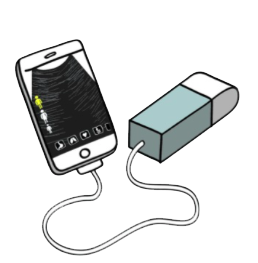
\includegraphics[scale=.65]{Images_Rapport/sonde2}\par 

\vspace{10pt}
% Include a department/university logo - this will require the graphicx package
Cette œuvre est mise à disposition sous licence Attribution -  Partage dans les Mêmes Conditions 3.0 France. Pour voir une copie de cette licence, visitez \url{http://creativecommons.org/licenses/by-sa/3.0/fr/} ou écrivez à Creative Commons, PO Box 1866, Mountain View, CA 94042, USA. 
%----------------------------------------------------------------------------------------

\vfill % Fill the rest of the page with whitespace

\end{titlepage}

\tableofcontents
\renewcommand{\headrulewidth}{1pt}
\fancyhead[R]{\textbf{Page \thepage}} 
\fancyhead[L]{\leftmark}

\renewcommand{\footrulewidth}{1pt}
\fancyfoot[R]{\textbf{Page \thepage}} 
\fancyfoot[L]{\leftmark}
\newpage
\section{Première partie: Approche scientifique }
\subsection{Problématique}

Parmi les grands enjeux sociétaux du XXI$^{eme}$ siècle il en est un qui tient une place centrale : celui de la santé et de son financement.\par 
Si d'après l'organisation mondiale de la santé la France est le pays qui présente le meilleur système de santé du monde elle présente encore néanmoins de profondes inégalités d'accès aux soins dues notamment à un fort gradient social et a des spécialistes mal répartis sur le territoire. Ce phénomène à pour conséquence dans un pays ou l'espérance de vie est l'une des plus élevée au monde d'avoir également un des taux de mortalité prématurée évitable les plus forts d'Europe. \par 

Au niveau mondial ou les inégalités se creusent encore davantage de nombreux pays n'offrent aujourd'hui pas encore la prestation d'une série de services de santé de base \cite{OMS1}.
En effet dans de nombreuses zones en développement de la planète la base de trop nombreux diagnostics est encore aujourd'hui composée de simples observations à l'oeil nu et palpations qui ne permettent pas seules de juger de l'urgence de certaines situations. \par

C'est dans ce contexte précis qu'un apport des techniques d'imagerie médicale est primordial et permettra de sauver de nombreuses vies. Cependant les principaux dispositifs d'imagerie d'aujourd'hui sont encombrants, couteux et utilisés par des médecins spécialisés. \par
Dans le but de toucher le plus grand nombre il faudrait apporter une solution économique, peu encombrante et utilisable facilement par des professionnels tels que les médecins généraliste en France qui sont souvent une personne de confiance très abordable pour les familles ou encore les membres d'associations telles que Médecins sans frontières présents dans les pays en voie de développement.\par
\vspace{10pt}

\par
\vspace{10pt}

\subsection{Contenu du dossier}

Ma collaboration avec le groupe echOpen s'étant principalement articulé en deux grandes phases, le premier objectif de ce dossier sera de les retranscrire. En effet  j'ai tout d'abord été amené à étudier activement en détail le fonctionnement de la sonde échographique développée pour répondre à la problématique(notamment du point de vue de sa chaine d'acquisition), puis en exploitant mes connaissances dans le domaine des convertisseurs statiques de puissance il m'a été demandé de proposer une solution qui permettrait d'effectivement rendre le système entièrement portable.\par
Le second objectif de ce dossier sera de présenter deux exploitations pédagogiques pour le cycle terminal et l'enseignement supérieur portant sur les deux phases de mon travail au sein d'echOpen. 


\newpage

\subsection{Présentation du projet echOpen}
\subsubsection{Structure}

La structure echOpen \cite{echopen} qui m'accueille dans le cadre de ce dossier industriel est un noyau de cinq personnes qui ont rassemblé autour d'elles une communauté de plus de 200 personnes dans le but de mener à bien leur projet de conception d'un écho-stéthoscope open source à bas cout.\par
Soutenu par la fondation Pierre Fabre et basé à l'hôpital Hôtel Dieu sur l'île de la cité à Paris le projet echOpen a vu le jour à l'automne 2014 avec pour objectif d'obtenir un premier prototype fonctionnel le 17 février 2016 soit le jour du bicentennaire de l'invention du stéthoscope par le docteur René Laënnec. \par
\vspace{10pt}

\begin{figure}[h!]
\centering
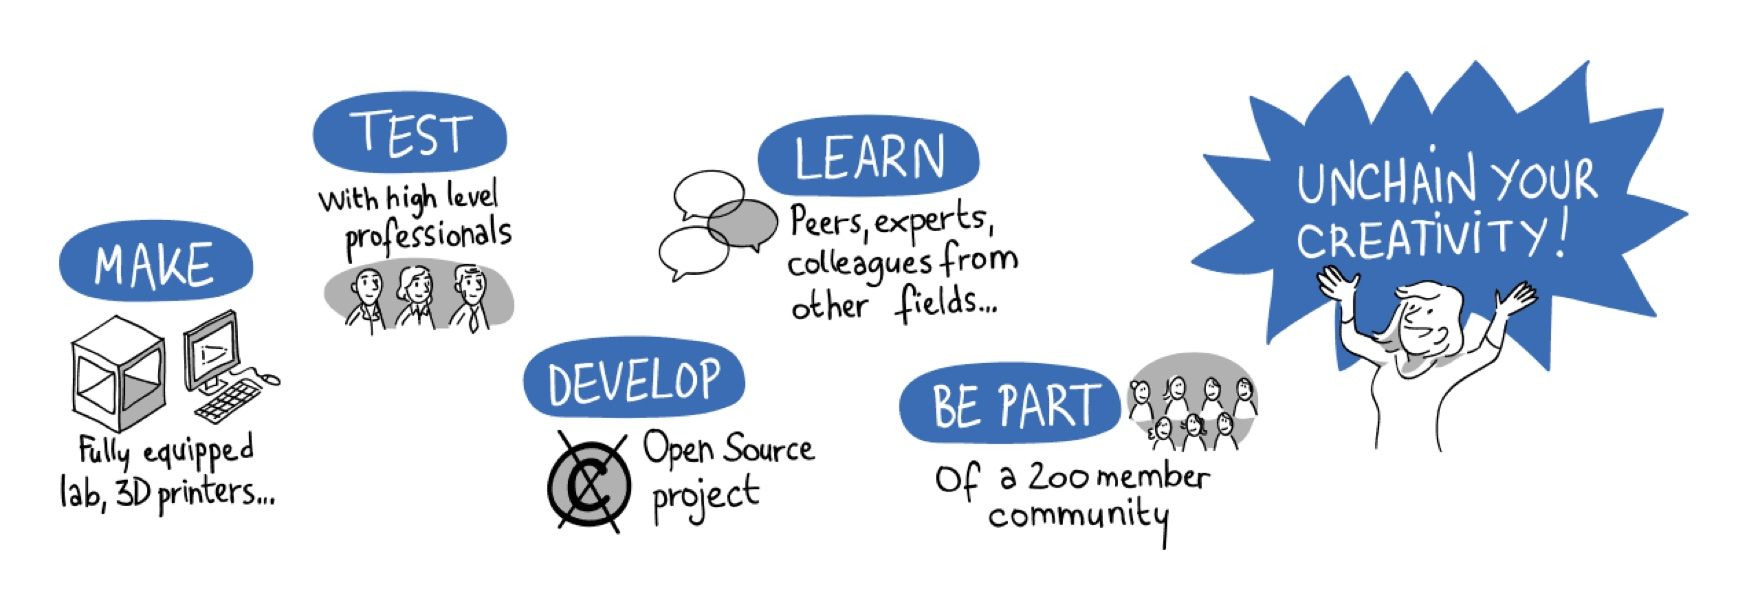
\includegraphics[scale=.29]{Images_Rapport/fonctionnement_echopen} 
\caption{Fonctionnement du projet echOpen}
\end{figure}

\subsubsection{Objectifs et contraintes}
\vspace{10pt}
A terme l'objectif principal du projet echOpen est de concevoir une sonde réalisant des échographies appelée écho-stéthoscope qui soit ultra portable, utilisable facilement par l'ensemble des personnels de santé (médecin de famille, infirmier, médecin de brousse, vétérinaire, ...) et dont les résultats soit directement visualisable sur un téléphone mobile afin que d'aider à établir des diagnostics plus fiables. \par 
Cependant il tient également à coeur aux fondateurs du projet que celui-ci ait une visée pédagogique et puisse servir de support à la formation des étudiants de tous niveaux. Le caractère open source du projet facilitant grandement la démarche.\par 
Ainsi ont peut résumer les usages fait du système support de ce dossier dans le diagramme suivant.\par


\vspace{20pt}
\begin{figure}[!h]
\hspace{-20pt}
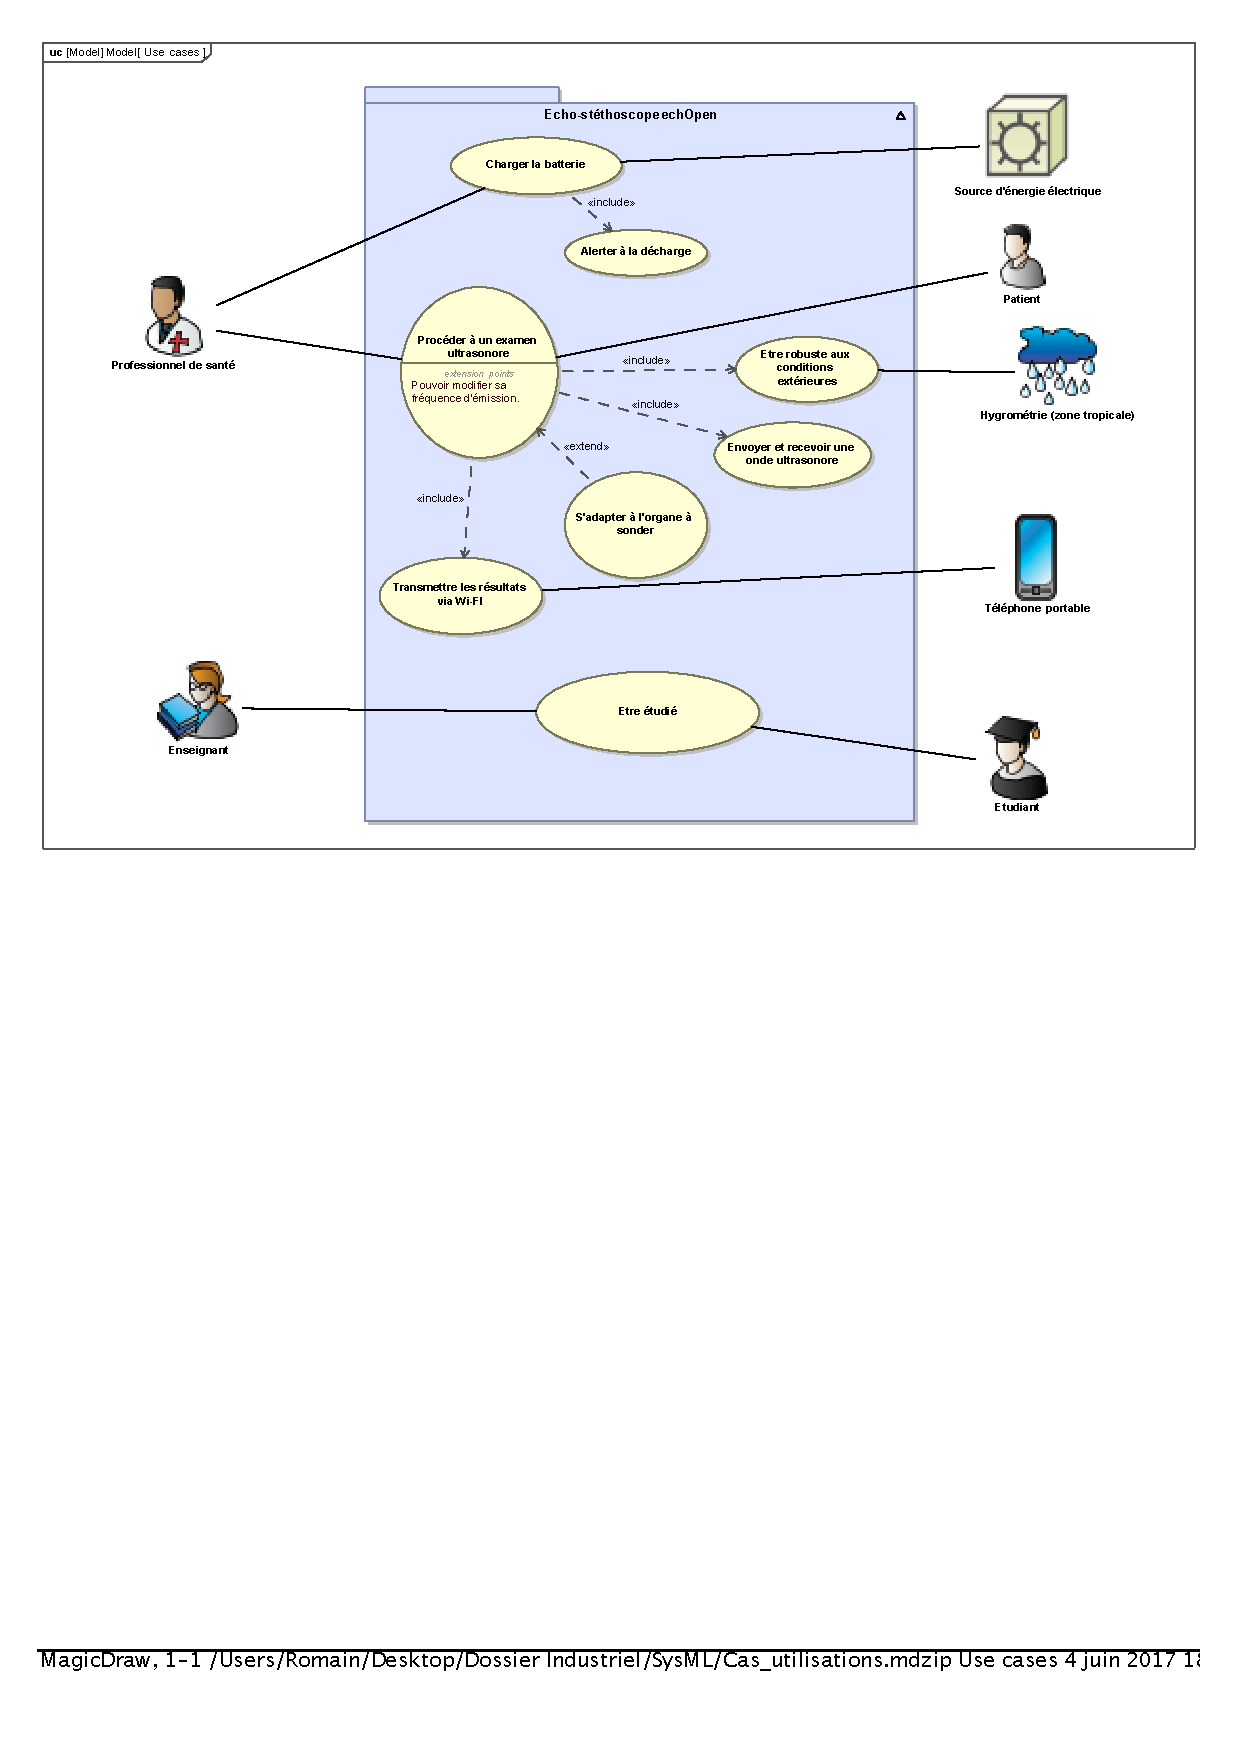
\includegraphics[width=19cm,trim=0cm 15cm 0cm 0cm, clip=true]{Images_Rapport/utilisations_pdf} 
\caption{Diagramme des cas d'utilisations}
\end{figure}

\newpage
\vspace{15pt}
\begin{wrapfigure}{r}{0.5\textwidth}
  \vspace{-0pt}
  \begin{center}
    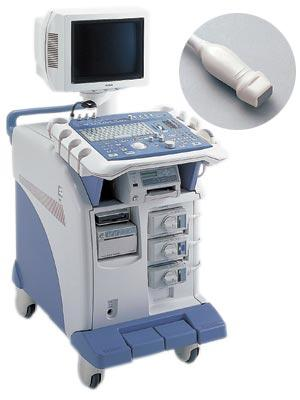
\includegraphics[width=0.18\textwidth]{Images_Rapport/echo}
  \end{center}
  \vspace{-5pt}
  \caption{Système d'échographie classique}
  \vspace{-10pt}
\end{wrapfigure}


\vspace{20pt}
Aujourd'hui encore même dans les pays les mieux équipés médicalement lorsqu'un patient doit faire une échographie il se rend chez un spécialiste possédant une machine de pointe. Afin d'obtenir le cahier des charges de notre système nous pouvons partir du mode de fonctionnement actuel et en déduire ce qu'il faut changer pour arriver à un système utilisable dans l'ensemble des cas précédemment cités. Les principales incompatibilités des dispositifs actuels avec nos objectifs sont: \par
\vspace{10pt}




\begin{itemize}
\item Le prix prohibitif : un dispositif d'échographie fixe est estimé entre 8000 et 15000 \euro{}
\item Le volume trop encombrant : le système actuel est encombrant et il est inconcevable de le déplacer hors d'un seul batiment.
\item La prise en main compliquée : le dispositif actuel propose de très nombreux paramètres réglables manuellement par le spécialiste.
\end{itemize}










\vspace{10pt}
\newpage
Partant de ces quelques constatations nous savons ainsi que nous devons réaliser un système facile à prendre en main (utilisable après 48 heures de formation), ultra portable (sortable d'une poche de blouse ou d'un tiroir lorsqu'on doit l'utiliser et compatible avec un smartphone pour l'affichage), économique (environ un dixième du prix actuel) mais également ayant une qualité d'image comparable aux solutions actuellement utilisées dans les hôpitaux. En regroupant ces quelques points et en en détaillant certains on aboutit ainsi au cahier des charges représenté sur le diagramme suivant.  \par
\vspace{15pt}



\begin{figure}[!h]
  \hspace{-25pt}
  \includegraphics[width=18cm,trim=1cm 18cm 8cm .75cm, clip=true]{Images_Rapport/cdc_pdf}
 
  
  \caption{Diagramme des exigences}
  
\end{figure}

\newpage

\subsection{Fonctionnement de l'écho-stéthoscope portable echOpen}

L'objectif de cette partie est de présenter le fonctionnement détaillé du système dans son état actuel de fonctionnement. L'amélioration du système étant toujours en cours il est intéressant de remarquer la présence de différences encore notables entre le cahier des charges final et les performances actuelles. Concretement le système actuel est parfaitement fonctionnel et permet déjà d'obtenir des images exploitables mais la sonde n'est pas encore dotée de toutes ses options et certains de ses paramètres sont encore optimisables.\par
\vspace{10pt}

\subsubsection{Principe de base de l'échographie}

\paragraph{Les ondes ultrasonores}
On appelle communement ultrasons les ondes sonores dont la fréquence est comprise dans la bande 20 kHz - 1 GHz. Pour le système présenté ici la fréquence choisie est de 3,5 MHz, elle se situe dans la bande des ultrasons dits de diagnostic utilisée en médecine qui couvre la bande [2-20] MHz.\par
Etant une onde mécanique de pression l'onde ultrasonore nécessite un milieu élastique déformable pour se propager et provoque lors de son passage des zones de détente et des zones de compression. On peut caractériser cette onde à l'aide de différents paramètres:\par
\vspace{10pt}

\begin{itemize}
\item Sa fréquence : $f = \dfrac{1}{T}$
\item Sa vitesse $v$ et sa longueur d'onde  $\lambda $ liées par la relation $\lambda = \dfrac{c}{f}$
\item Sa pression P et son intensité I liées par la relation $I = \dfrac{P^2}{2Z}$ ou Z est appelée impédance acoustique du milieu traversé [$Pa.s.m^{-1}$]. Pour une onde plane progressive l'impédance acoustique du milieu traversé est lié à sa masse volumique $\rho$ et à la vitesse de propagation de l'onde par la relation $Z = \rho .v$
\end{itemize}
\vspace{10pt}
Les ondes ultrasonores obéissent aux lois de Snell-Descartes concernant la réflexion et la réfraction, peuvent subir de la diffusion omnidirectionnelle (ou de Rayleigh) en cas de rencontre avec de petites particules ou des surfaces granuleuses et sont assez fortement atténuées et absorbées dans le milieux organiques.\par
\vspace{10pt}

La technique d'échographie exploite les ondes réfléchies revenant vers le récepteur. Comme ce récepteur est également l'émetteur on peut alors raisonnablement faire l'hypothèse que ces ondes ont une incidence normale aux milieux rencontrés. On peut alors définir le coefficient de réflexion de l'onde ultrasonore à l'interface entre deux milieux 1 et 2 par :

\[\Gamma = \dfrac{I_{reflechie}}{I_{incidente}} = \dfrac{(Z_2-Z_1)^2}{(Z_1+Z_2)^2}\]

\vspace{10pt}

Ainsi en considérant une vitesse de propagation des ondes à peu près identique dans l'ensemble des milieux organiques (on considère la vitesse de propagation dans l'eau qui compose majoritairement le corps humain et qui est de 1460 $m.s^{-1}$ tandis que dans les faits pour l'ensemble des corps mous du corps humain il existe une dispersion de $\pm$ 10 $m.s^{-1}$ autour de cette valeur) l'étude de l'intensité du signal réfléchi et donc de son enveloppe donne directement une indication de l'impédance acoustique des milieux rencontrés et indirectement leur masse volumique.   \par

\vspace{10pt}

\begin{figure}[!h]
  \vspace{-0pt}
  \begin{center}
    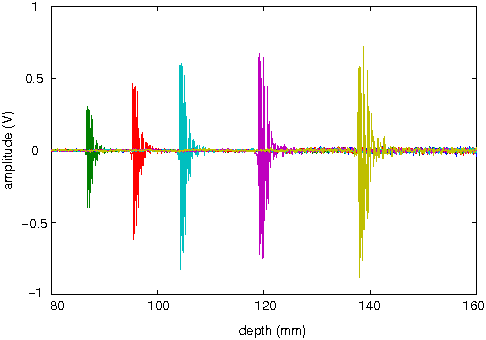
\includegraphics[width=14cm]{Images_Rapport/sig}
  \end{center}
  
  \caption{Allure typique de l'image électrique des signaux réfléchis}
  
\end{figure}

La figure ci-dessus montre les échos renvoyés par une plaque métallique au transducteur. Chaque couleur correspond à une mesure distincte pour laquelle la plaque à été déplacée. \par
\vspace{10pt}

\underline{\textbf{Remarque:}} Ici l'atténuation en fonction de la distance n'est pas visible car une méthode d'amplification à gain variable est déjà mise en place. Cette image valide donc juste le fait que l'on détecte la position d'une interface mais on ne peut pas conclure uniquement grâce à elle que l'on connait aussi la nature de l'interface.\par
\vspace{10pt}

Le tableau suivant recense quelques valeurs numériques d'impédance acoustique des principaux milieux rencontrés dans le domaine médical.
\begin{center}
\begin{tabular}{|c|c|}
  \hline
  Milieu & Impédance acoustique ($kg.m^{-2}.s^{-1}$) \\
  \hline
  Air & $4.10^{2}$ \\ \hline
  Poumon & $0.26.10^{6}$  \\
  \hline
  Os & $3,8-7,4.10^{6}$ \\ \hline
  Tissus mous & $1,3-1,7.10^{6}$  \\
  \hline
  Eau & $1,5.10^{6}$ \\ \hline
 
\end{tabular}
\end{center}

\vspace{10pt}

\underline{\textbf{Remarque:}} La différence notable d'impédance acoustique entre les tissus humains et l'air reportée dans la formule du coefficient de réflexion précédemment définie interdit la présence de celui-ci sur le chemin de l'onde ultrasonore. En effet une interface air/milieu organique implique une réflexion totale qui fausse immédiatement toute mesure.

\newpage
\paragraph{L'émetteur/récepteur : le transducteur piézo-électrique}

L'émission et la réception des ondes ultrasonores est possible grâce un transducteur piézo-électrique focalisé (sa surface est très légèrement incurvée) de distance focale 12 cm et de fréquence de résonance 3,5 MHz ($f = \dfrac{K}{e}$ avec K constante matériau et e l'épaisseur de la céramique). 
Ce transducteur permet l'exploration des zones les plus profondes du corps humain jusqu'à 20 cm mais est peu performant pour les zones situées juste sous la peau. Une vue en coupe de ce transducteur est donnée à la figure suivante.

\begin{figure}[!h]
  \vspace{-0pt}
  \begin{center}
    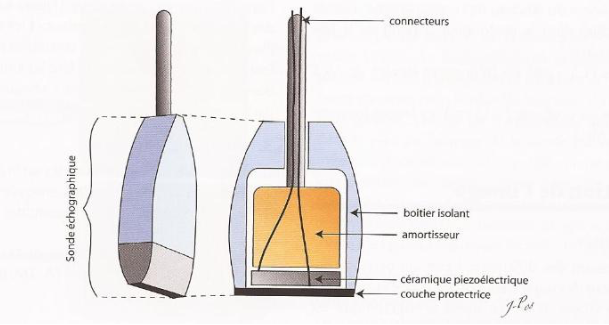
\includegraphics[width=15cm]{Images_Rapport/transducteurs}
  \end{center}
  
  \caption{Composition d'une sonde échographique \cite{sonde}}
  
\end{figure}

Tout le principe physique de la sonde est basé sur le fait que la céramique piézo-électrique permet d'exploiter l'effet piézo-électrique direct (pression acoustique $\rightarrow$ Force $\rightarrow$ Polarisation du transducteur) en réception et l'effet piézo-électrique indirect (Différence de potentiel appliquée $\rightarrow$ Contraction brusque de la céramique $\rightarrow$ Emission d'une onde acoustique) en émission. Cependant il est nécessaire d'entourer ce composant de protections pour le bon fonctionnement de la sonde : le boitier isolant assure le fait que l'air n'est pas présent sur le parcours des ondes acoustiques, l'amortisseur réduit fortement les réflexions d'ondes à l'arrière de la céramique dans le boitier et la couche protectrice permet d'introduire une impédance intermédiaire entre celle de la céramique et celle du milieu sondé. Cette couche est recouverte de gel afin d'assurer un contact parfait entre la peau et la sonde. \par 
\vspace{10pt}

\underline{\textbf{Remarque:}} Dans le but de simplifier les procédures de test il est possible de se séparer du gel échographique et de la couche protectrice en plongeant simplement l'ensemble du dispositif dans l'eau.
\newpage
\subsubsection{Fonctionnement du système complet}

Maintenant que nous connaissons le phénomène physique exploité afin de réaliser les échographie ainsi que le capteur permettant de recevoir les échos ultrasonores nous pouvons voir dans quel environnement nous le mettons en oeuvre. La version du système présentée ici est décomposable en deux parties : le corps de la sonde chargé d'acquérir et de conditionner les données et une application mobile chargée de les traiter et de les restituer via l'écran. La partie suivante s'attache principalement à expliquer l'ensemble des fonctions réalisées dans le corps de la sonde. \par

\vspace{10pt}

\begin{figure}[!h]
  \hspace{-60pt}
  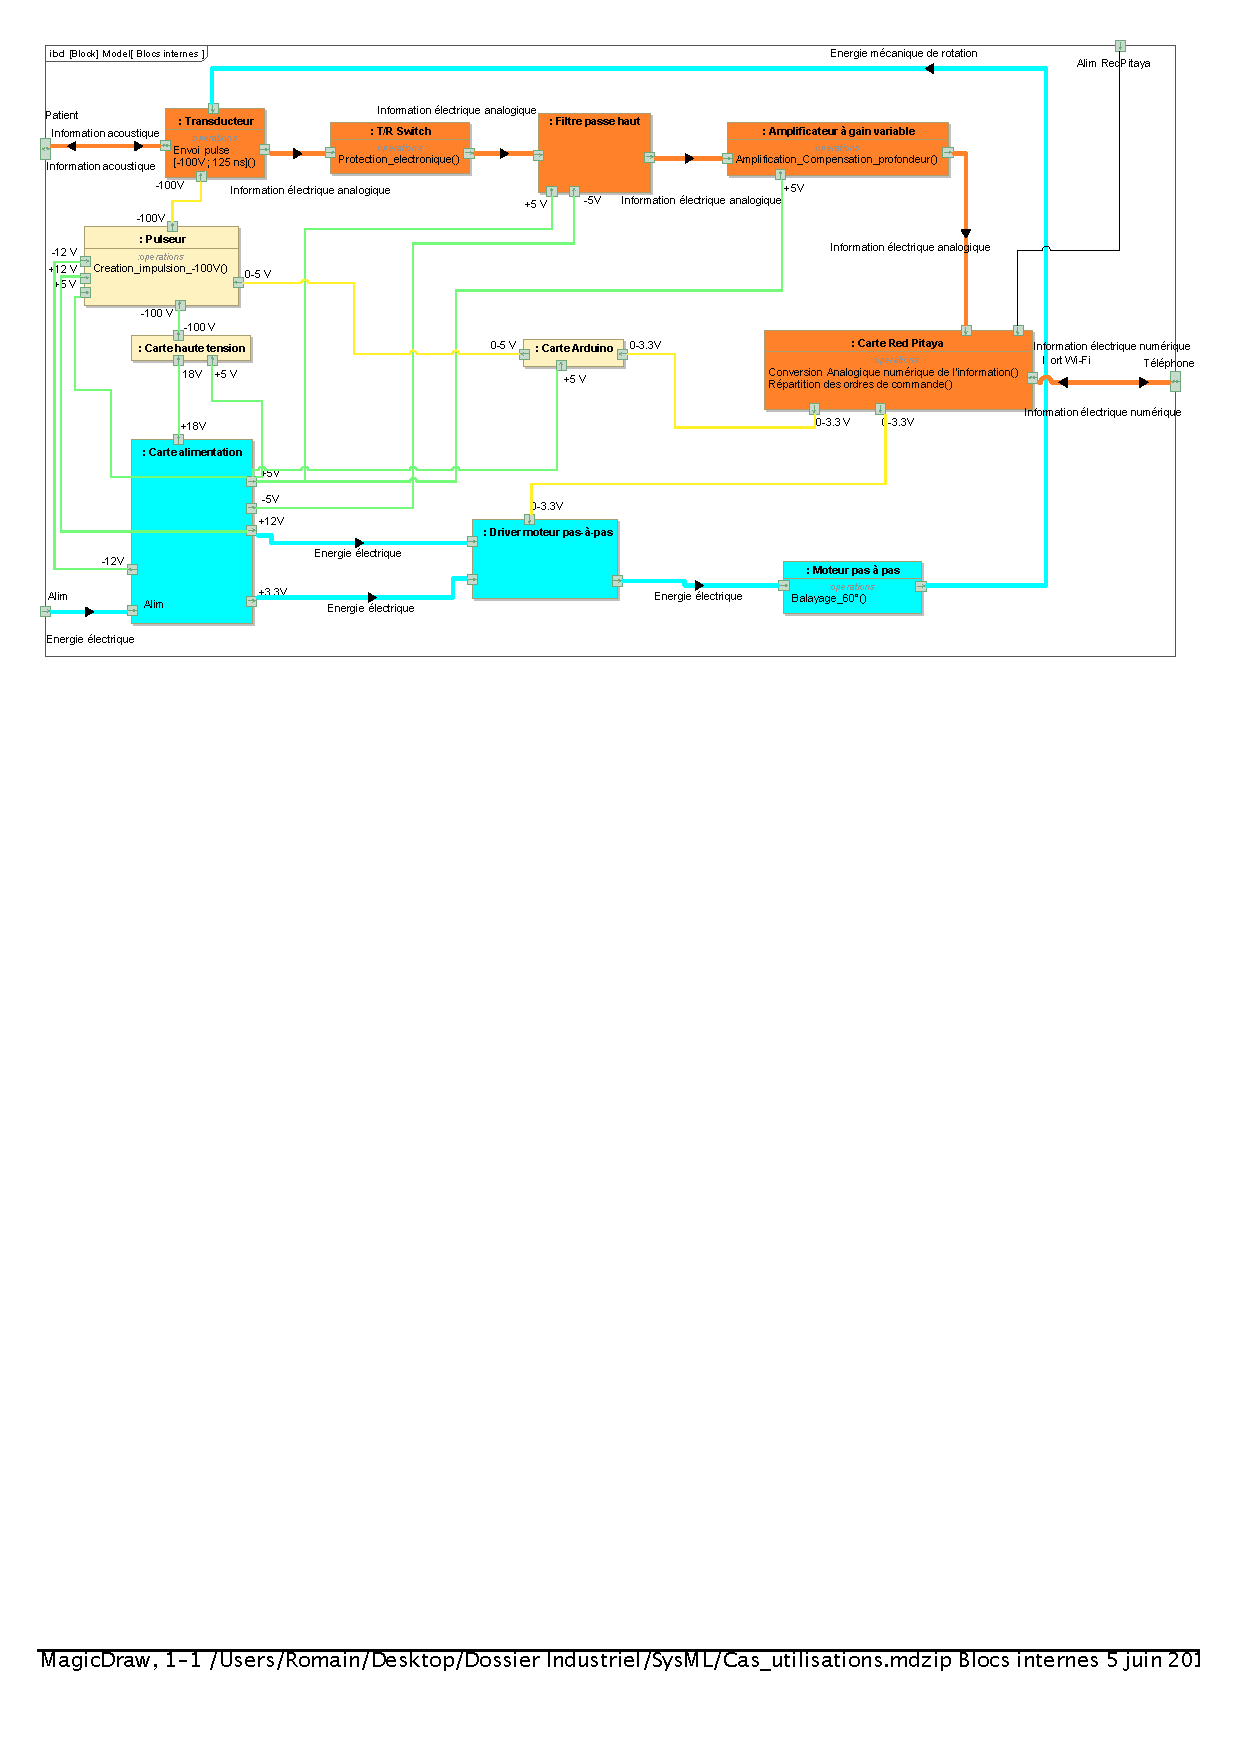
\includegraphics[width=21cm,trim=.5cm 18cm .5cm 0cm, clip=true]{Images_Rapport/ibdd}
  
  
  \caption{Diagramme de blocs internes de la sonde}
  
\end{figure}


\paragraph{La chaine d'énergie}

Représentée en bleu sur le diagramme de blocs internes la chaine d'énergie du système permet de faire tourner le transducteur dans le but d'acquérir les données échographiques.\par
En effet le transducteur choisi étant unique et focalisé il ne peut effectuer qu'une seule ligne de mesure. Afin de reconstituer une image il faut donc faire tourner le transducteur au fur et à mesure que l'on effectue des acquisitions.\par
\newpage
\begin{wrapfigure}{r}{0.5\textwidth}
  \vspace{-30pt}
  \begin{center}
    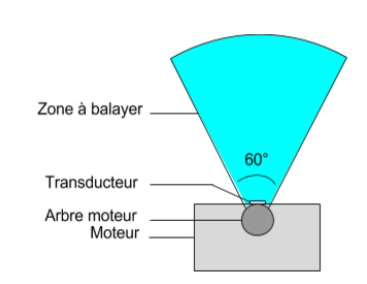
\includegraphics[width=0.28\textwidth]{Images_Rapport/balayage}
  \end{center}
  \vspace{-5pt}
  \caption{Mouvement de balayage}
  \vspace{-10pt}
\end{wrapfigure}
\vspace{10pt}
Pour cela on utilise un moteur pas à pas et son driver alimentés par une carte fournissant les niveaux de tensions adéquat et pilotés par la carte Red Pitaya.
Dans cette version de laboratoire l'énergie fournie à la carte d'alimentation provient encore d'une source de tension stabilisée. Cette solution est à changer et fera l'objet de la partie "apport personnel" présentée ci après.\par


\vspace{20pt}
\paragraph{La fabrication des impulsions}

Afin de pouvoir émettre une onde acoustique notre transducteur à besoin d'être fortement polarisé pendant une durée très courte. En effet afin d'obtenir une onde ultrasonore adapté à nos mesures nous devons envoyer une impulsion de -100V et de 125 ns au transducteur.\par


\begin{wrapfigure}[11]{l}{0.5\textwidth}
  \vspace{-50pt}
  \hspace{-20pt}
  \begin{center}
    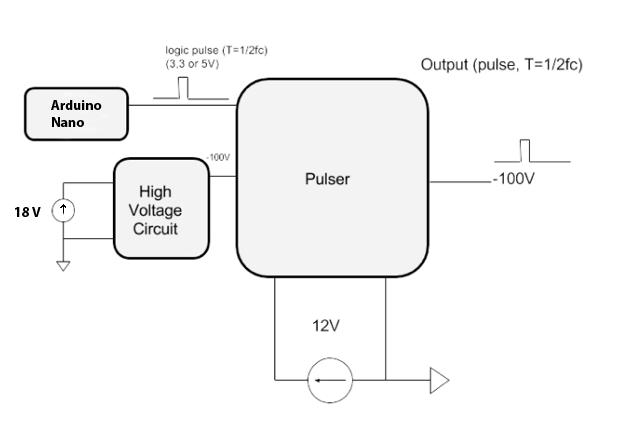
\includegraphics[width=0.52\textwidth]{Images_Rapport/hv}
  \end{center}
  \vspace{-5pt}
  \caption{Création d'un pulse}
  \vspace{-10pt}
\end{wrapfigure}


\vspace{15pt}
Pour cela nous disposons d'une carte dite de "haute tension" qui à pour rôle de fabriquer une tension continue de -100V. Nous disposons également d'une carte Arduino Nano chargée de créer des impulsions logiques (0-5V) de durée 125 ns. Enfin la carte appelée pulseur exploite l'information logique provenant de la carte Arduino nano et le niveau de tension provenant de la carte haute tension (HV) afin de créer une impulsion d'amplitude et de durée souhaitée.
\vspace{30pt}

\begin{figure}[!h]
  \hspace{-30pt}
  \vspace{30pt}
  \begin{minipage}[b]{0.45\linewidth}
   \centering
   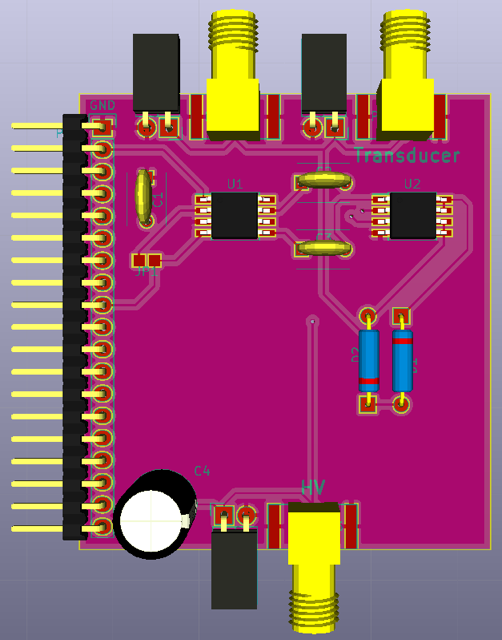
\includegraphics[width=9cm,height=7cm]{Images_rapport/pulseur}  
   \caption{Pulseur}   
  \end{minipage}
\hfill
  \begin{minipage}[b]{0.45\linewidth}
   \centering
   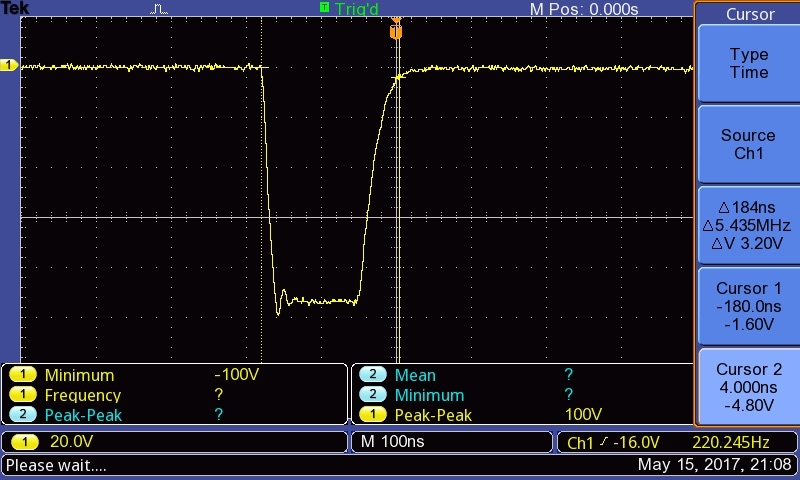
\includegraphics[width=9cm,height=7cm]{Images_rapport/pulse}  
   \caption{Une impulsion}   
  \end{minipage}
\end{figure}



%L'ensemble du processus de fabrication des impulsions est monitoré par la carte Red Pitaya qui coordonne l'ensemble du fonctionnement du système.


\newpage
\paragraph{La chaine d'acquisition}

Dans une sonde échographique, la chaine d'acquisition représente le coeur du système. Elle conditionne fortement la qualité des images que l'on va pouvoir créer et joue ainsi sur la qualité du diagnostic fournit au patient.

\begin{figure}[!h]
  \hspace{-60pt}
  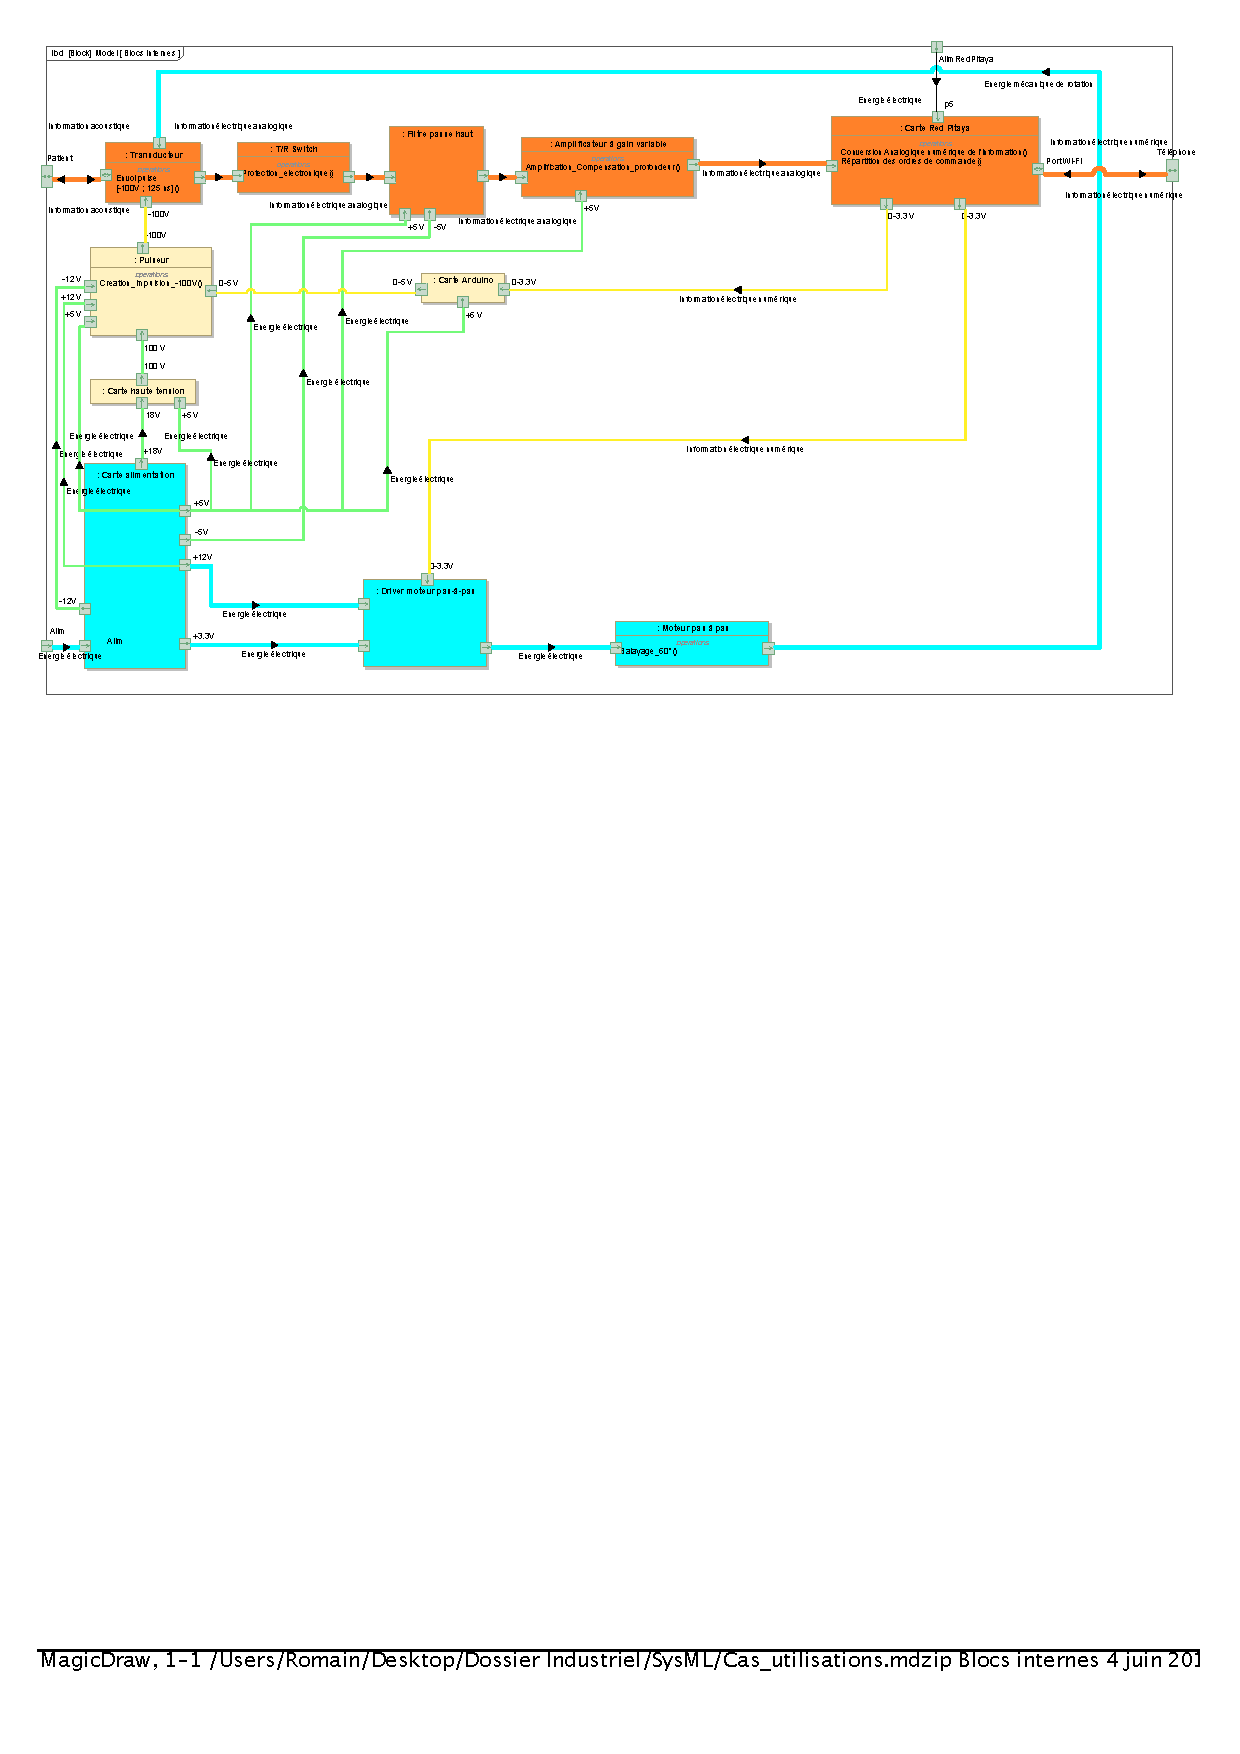
\includegraphics[width=21cm,height=4cm,trim=0cm 25.5cm 0cm 1.5cm, clip=true]{Images_Rapport/ibd_pdf}
  
  
  \caption{Chaine d'informations du système}
  
\end{figure}

Une fois qu'une impulsion à été générée, le transducteur se met en mode écoute, réceptionne les échos et en fabrique l'image électrique.\par
L'allure du signal (impulsion + échos) est donnée figure 13.

\begin{figure}[!h]
  \centering
  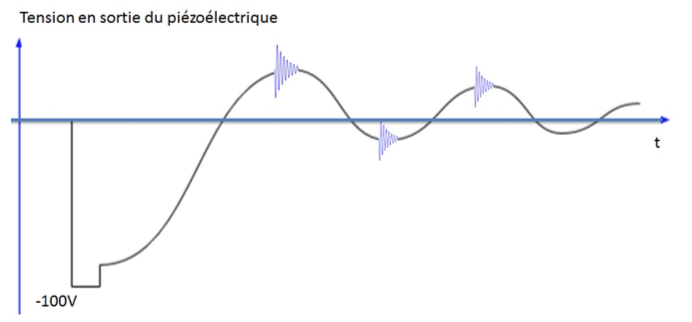
\includegraphics[width=14cm,trim=0cm 0cm 0cm 0cm, clip=true]{Images_Rapport/allure}
  
  
  \caption{Allure du signal en sortie du transducteur}
  
\end{figure}

Nous constatons qu'en plus des échos porteurs de l'information à 3,5 MHz un autre phénomène périodique de fréquence de l'ordre de la centaine de kHz apparait.\par
\vspace{20pt}

Ce signal issu du transducteur passe ensuite par les composants suivants:\par
\vspace{10pt}

\textbf{\underline{T/R Switch}} : Littéralement Transmit/Receive Switch ce composant sert à protéger l'électronique en aval des fortes tensions générées lors de l'émission et qui pourraient potentiellement se propager. Il agit simplement comme un interrupteur qui s'ouvre dès que la différence de potentiel à ses bornes est supérieure en valeur absolue à 2V.\par

\vspace{10pt}
\newpage

\begin{wrapfigure}[6]{r}{0.5\textwidth}
  \vspace{-30pt}
  \hspace{-0pt}
  \begin{center}
    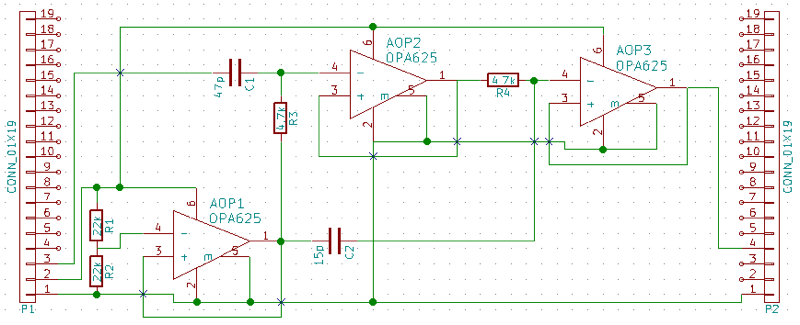
\includegraphics[width=0.52\textwidth]{Images_Rapport/passehaut}
  \end{center}
  \vspace{-5pt}
  \caption{Filtre passe haut}
  \vspace{-10pt}
\end{wrapfigure}
\textbf{\underline{Filtre passe haut}} : Ce filtre réalisé à partir d'une technologie active est de type passe haut et possède une fréquence de coupure de 500 kHz. Il est utilisé afin de supprimer la composante périodique à 100 kHz vue précédemment en sortir du transducteur.\par
\vspace{60pt}

\textbf{\underline{Amplificateur à gain variable}} : Appelé T.G.C pour Time Gain Control cet amplificateur possède une amplification variable en fonction du temps. Utilisé pour compenser l'atténuation dans les milieux organiques nous le pilotons via une loi qui agit directement sur son gain en dB (commande de 0V pour une amplification minimale de 7,5 dB et 1V pour une amplification maximale de 55.5 dB). \par 
Sachant que notre transducteur est utile entre 8 et 16 cm de profondeur notre loi de commande est donc linéaire entre 55 $\mu s$ et 110 $\mu s$ après émission du pulse en considérant une vitesse de propagation moyenne de 1460 $m.s^{-1}$.

\begin{figure}[!h]
  \centering
  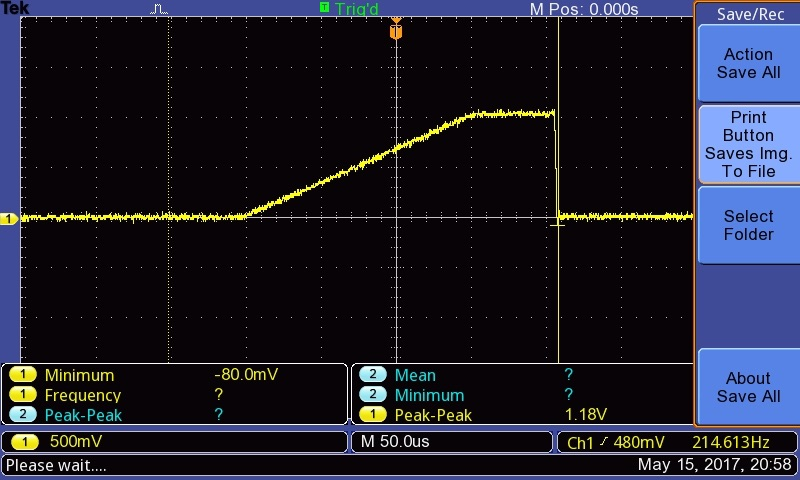
\includegraphics[width=12cm,trim=0cm 0cm 0cm 0cm, clip=true]{Images_Rapport/tgc}
  
  
  \caption{Loi de commande du T.G.C.}
  
\end{figure}
\vspace{20pt}


\begin{wrapfigure}[6]{r}{0.5\textwidth}
  \vspace{-50pt}
  \hspace{-0pt}
  \begin{center}
    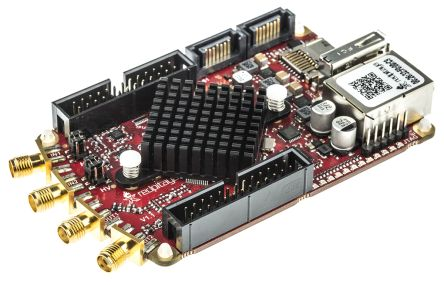
\includegraphics[width=0.42\textwidth]{Images_Rapport/redpitaya}
  \end{center}
  \vspace{-5pt}
  \caption{Carte Red Pitaya}
  \vspace{-10pt}
\end{wrapfigure}
\textbf{\underline{Carte Red Pitaya}} : La carte Red Pitaya est chargée d'effectuer la conversion analogique numérique (14 bits) du signal. Embarquant un micro serveur elle envoi ensuite les données numérisées via Wi-Fi au téléphone portable en utilisant le protocole TCP/IP.\par 

\newpage

Les données numériques arrivent ainsi ligne de mesure par ligne de mesure à l'application présente sur le téléphone portable qui effectue successivement les opérations suivantes:\par


\vspace{10pt}

\begin{itemize}
\item Filtrage numérique de type passe bande (BP = [1-6] MHz)
\item Détection d'enveloppe numérique (via Transformée de Hilbert) afin de récupérer l'énergie du signal.
\item Stockage des lignes dans une matrice. 
\item Attribution d'un niveau de gris pour chaque niveau de tension de l'enveloppe, mise en forme et affichage de l'image (Echographie Mode B pour Brillance)
\end{itemize}

\paragraph{Séquence de fonctionnement}

Afin de mieux saisir l'ensemble du fonctionnement du système lorsqu'un professionnel de santé a appliqué la sonde et utilise son smartphone pour visualiser une échographie en temps réel et en continu un diagramme de séquence est présenté en annexe 1.


\paragraph{Résultats obtenus}

Lors des derniers essais publics réalisés fin 2016 avec la version du kit présente ci-dessous les résultats obtenus étaient les suivants.\par

\vspace{10pt}

\begin{figure}[!h]
  \hspace{-30pt}
  \vspace{30pt}
  \begin{minipage}[b]{0.45\linewidth}
   \centering
   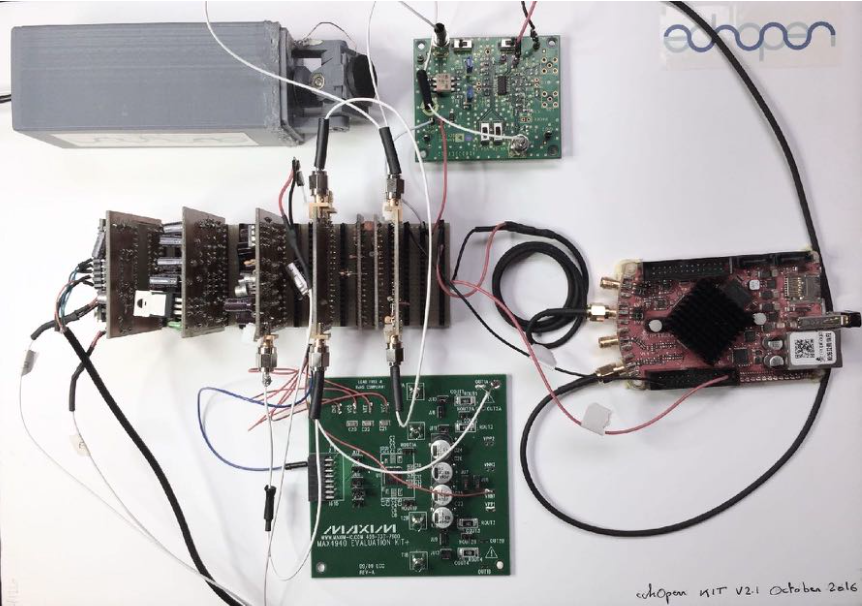
\includegraphics[width=9cm,height=8cm]{Images_rapport/kit}  
   \caption{Kit echOpen Fin 2016}   
  \end{minipage}
\hfill
  \begin{minipage}[b]{0.45\linewidth}
   \centering
   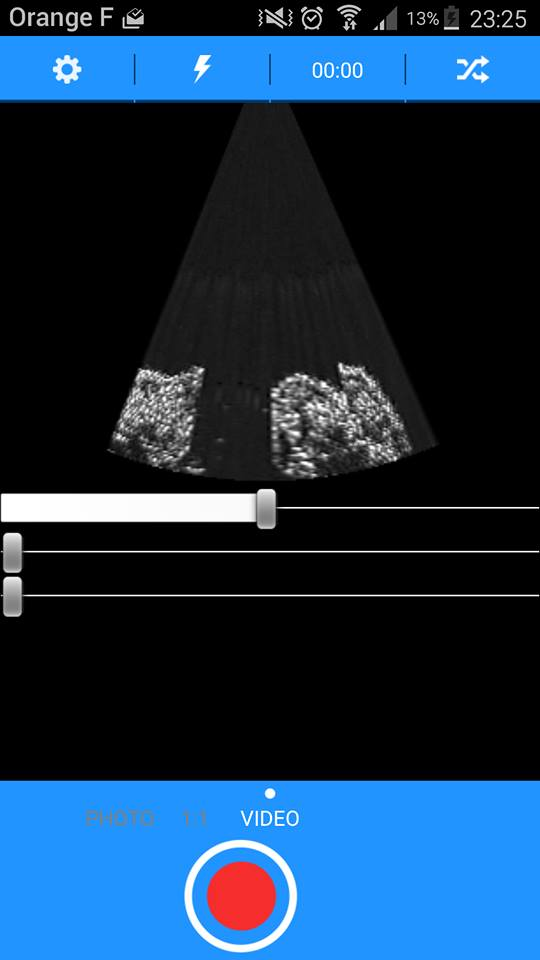
\includegraphics[width=9cm,height=8cm]{Images_rapport/result}  
   \caption{Image obtenue}   
  \end{minipage}
\end{figure}

\newpage
\subsection{Apport personnel}
\subsubsection{Problématique}

La version du système présentée jusque la et composée de deux unités physiques (corps de sonde + téléphone portable) est encore celle considérée comme la dernière en date pour l'ensemble de la communauté mais ceci devrait rapidement changer pour une version comportant trois unités physiques grâce au travail que j'ai effectué et que je présente dans cette partie. En effet le corps de la sonde est pour le moment alimenté via une source de tension stabilisée non adaptée à la caractéristique portable du système c'est pourquoi j'ai été amené à proposer le système suivant.\par

\vspace{20pt}
\begin{wrapfigure}[4]{r}{0.5\textwidth}
  \vspace{-40pt}
  \hspace{-0pt}
  \begin{center}
    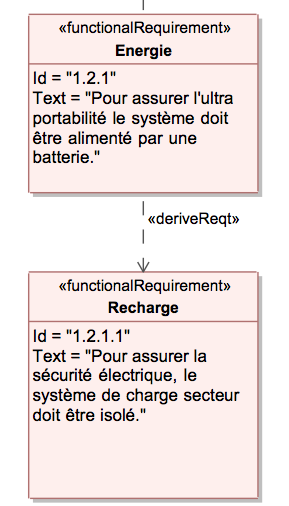
\includegraphics[width=0.22\textwidth]{Images_Rapport/portabilites}
  \end{center}
  \vspace{-5pt}
  \caption{Exigences énergie}
  \vspace{-10pt}
\end{wrapfigure}

En se basant sur les exigences du cahier des charges rappelées ci-contre il m'a donc été demandé de pourvoir une solution économique d'apport d'énergie au système.\par
\vspace{10pt}
\begin{tabular}{|c|c|}
  \hline
  Contrainte & Valeur  \\
  \hline
  $V_{in}$ & 110-230 $V_{eff}$ - 50-60 Hz \\ \hline
  $V_{out}$ & 18 $V_{DC}$  \\
  \hline
  Puissance & 18 W \\ \hline
  Isolation & Oui  \\
  \hline
 
 
\end{tabular}
\vspace{100pt}

La solution proposée devra être capable de substituer directement la source de tension stabilisée de laboratoire mais également de pouvoir charger une batterie équipée de son système de gestion (B.M.S. : Battery Management System).
\subsubsection{Topologie de la solution proposée}

Si il est aisé et très économique de fabriquer une tension continue de 18 V à partir d'un réseau d'alimentation public à l'aide de simples diodes (Pont de Graëtz) et de régulateurs cette solution n'est pas envisageable car elle ne propose pas \textbf{la fonction isolation} primordiale lorsqu'on souhaite vendre un système respectant la sécurité des personnes.\par
\vspace{10pt}


\begin{wrapfigure}[6]{r}{0.5\textwidth}
  \vspace{-50pt}
  \hspace{-0pt}
  \begin{center}
    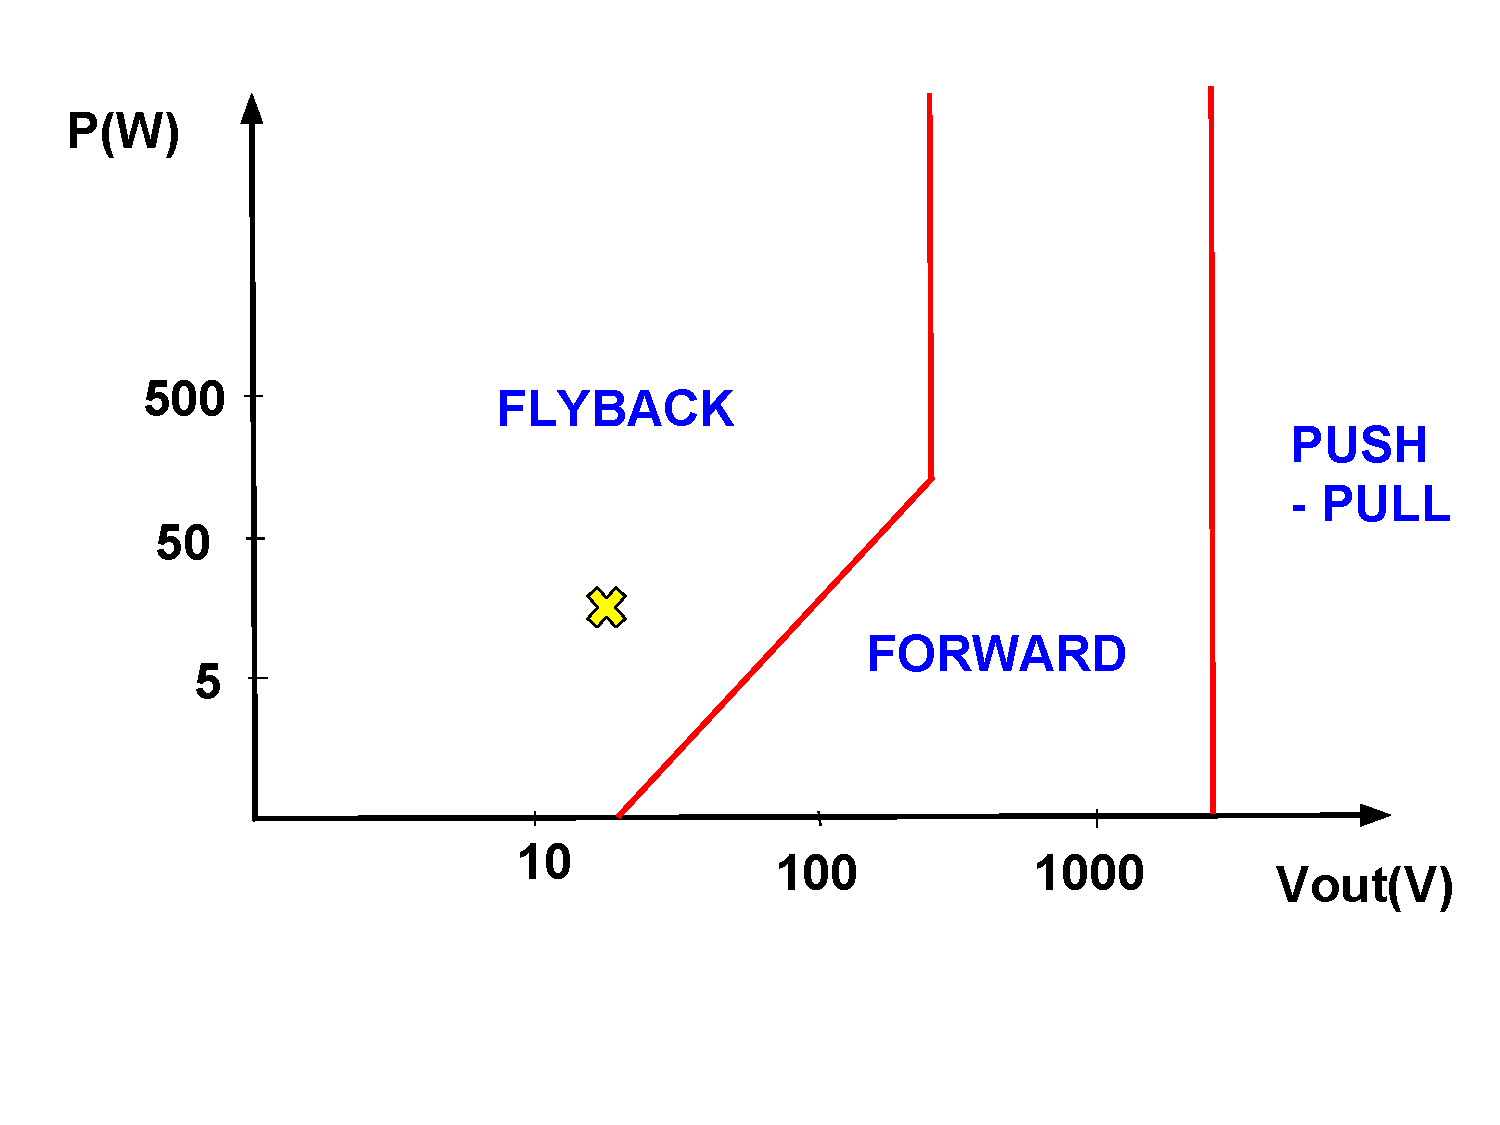
\includegraphics[width=6cm,trim=0cm 3cm 0cm 0cm, clip=true]{Images_Rapport/choix3}
  \end{center}
  \vspace{-5pt}
  \caption{Choix d'une topologie}
  \vspace{-10pt}
\end{wrapfigure}

\vspace{20pt}
Partant de ce constat on se tourne alors vers une alimentation à découpage isolée. De plus le faible calibre en puissance et tension de sortie pousse logiquement à choisir la solution la plus simple et la plus économique à savoir \textbf{le convertisseur Flyback}.\par
\vspace{85pt}
La structure Flyback est un convertisseur DC-DC isolé. Dans notre cas la source d'énergie étant un réseau alternatif il faut lui associer un convertisseur AC-DC. Etant donné la faible puissance demandée par la sonde l'utilisation d'un pont redresseur capacité en tête ne pose pas de problème vis-à-vis de la norme EN 61000-3-2 qui régit l'amplitude des courants harmoniques renvoyés au réseau.\par
\vspace{ 10pt}


\begin{figure}[!h]
  \hspace{-30pt}
  \vspace{-30pt}
  \begin{minipage}[b]{0.45\linewidth}
   \centering
   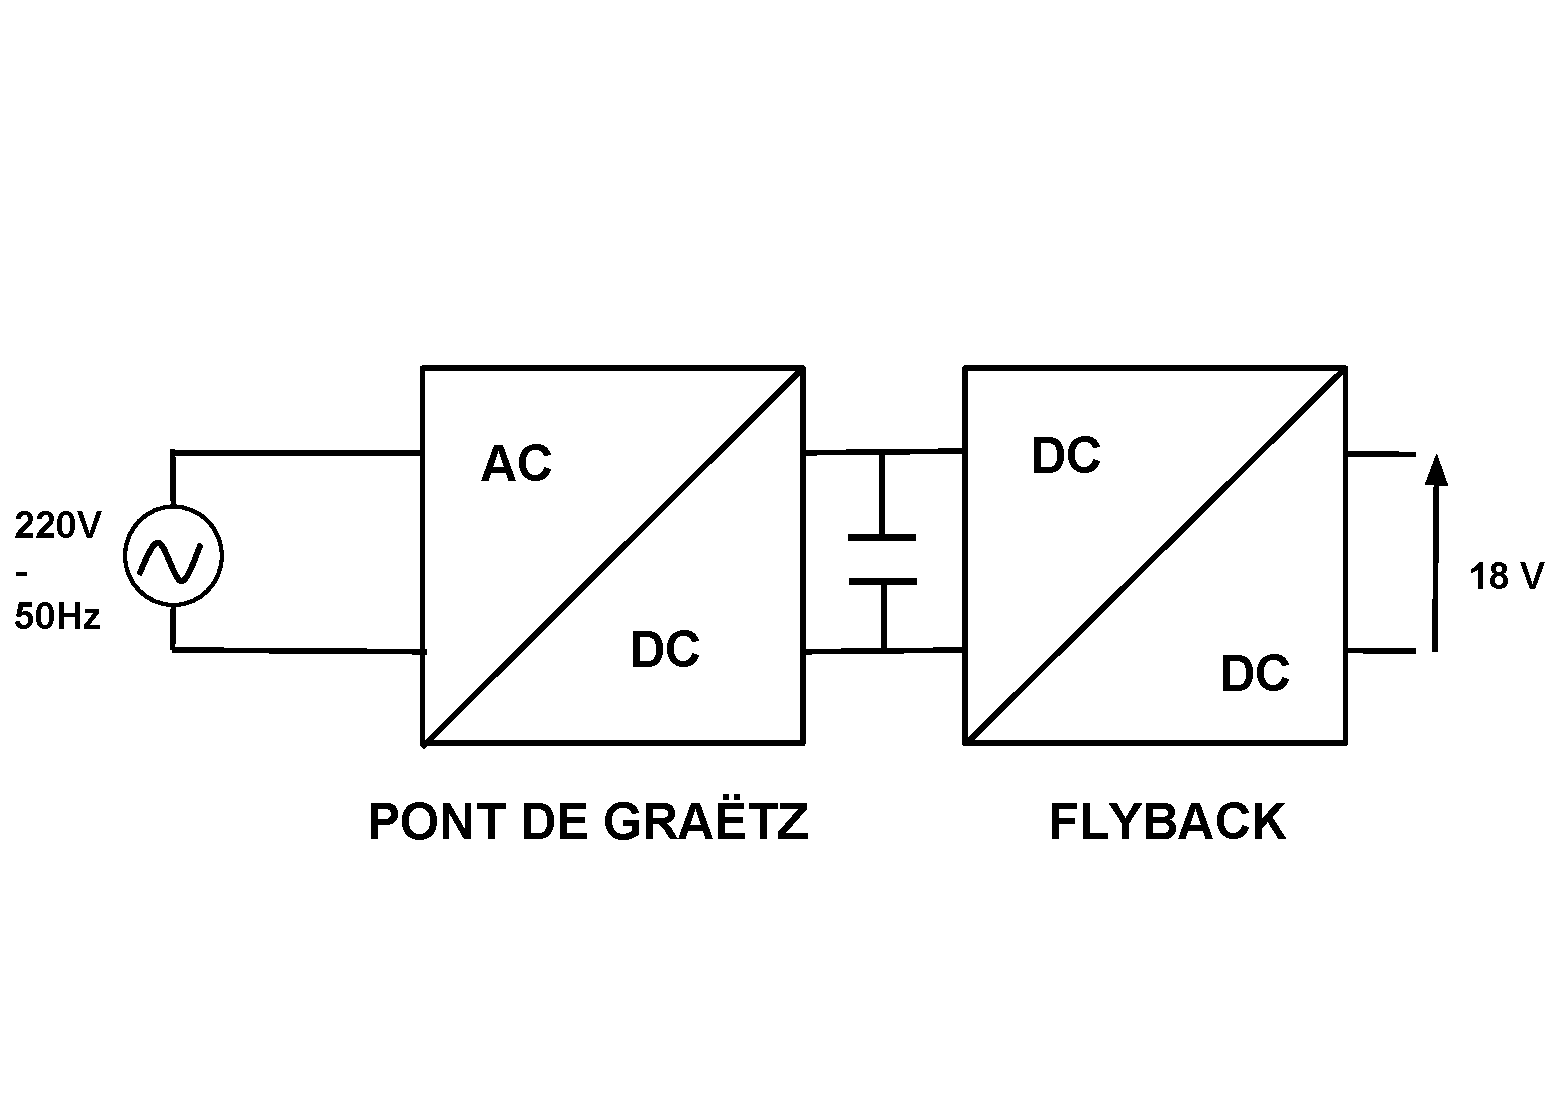
\includegraphics[width=9cm,height=5cm,trim=0cm 3cm 0cm 4cm, clip=true]{Images_rapport/conversion}  
   \caption{Structure générale}   
  \end{minipage}
\hfill
  \begin{minipage}[b]{0.45\linewidth}
   \centering
   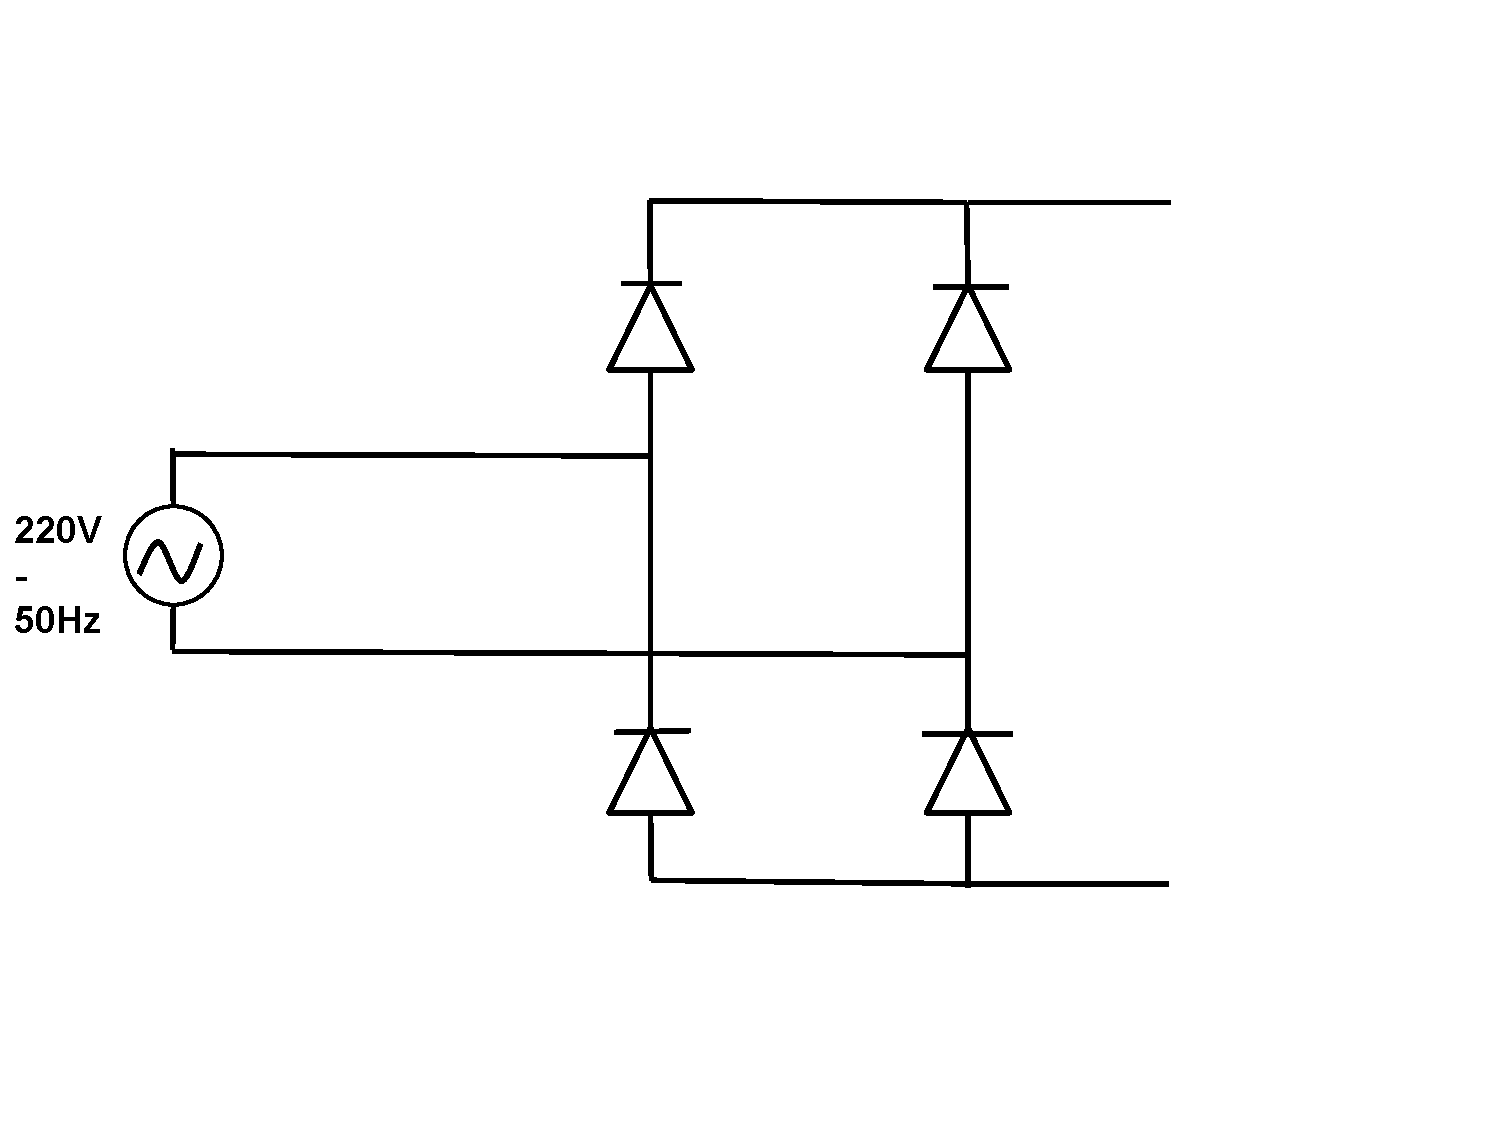
\includegraphics[width=9cm,height=5cm,trim=0cm 3cm 0cm 3.3cm, clip=true]{Images_rapport/redresseur}  
   \caption{Redresseur}   
  \end{minipage}
\end{figure}
\vspace{40pt}




La structure générale d'un convertisseur Flyback (également Buck-Boost isolé) est donnée figure 24 ci-après. Dans cette représentation Ve modélise l'ensemble {réseau + redresseur + condensateur} en amont et R la charge associée au convertisseur.

\begin{figure}[!h]
  \centering
  
\includegraphics[width=12cm,trim=0cm 0cm 0cm 0cm, clip=true]{Images_Rapport/flyback}
  
  
  \caption{Structure générale d'un convertisseur Flyback}
  
\end{figure}

Ce montage fonctionne selon le principe des vases communiquants. L'interrupteur T est fermé et la diode bloquée pendant une première phase et un courant s'installe dans la maille d'entrée, un flux est alors produit par l'enroulement primaire des inductances couplées $L_1$ et $L_2$. Au cours d'une seconde phase l'interrupteur est ouvert. Pour assurer la continuité du flux magnétique ($n_1.I_{1M} = n_2.I_{2M}$) la diode entre alors en conduction. \par
On parle d'inductances couplées car au cours d'un cycle de fonctionnement ou période de découpage les deux enroulements ne sont pas simultanément parcourus par un courant. Ce mode de fonctionnement nécessite un circuit magnétique avec entrefer afin de stocker l'énergie. \par


\vspace{10pt}

\subsubsection{Dimensionnement de la structure}
\paragraph{Principe de fonctionnement rapide}

Dans cette structure à découpage le transistor servant d'interruteur commute à une fréquence $F_{dec}$ et est fermé pendant une portion $\alpha$ ($\alpha \in [0;1]$) de la période de découpage $T_{dec}$. On considère de plus que le flux dans les enroulements ne s'annulera jamais, on se place donc en conduction continue ou démagnétisation incomplète.  \par
\vspace{10pt}

On a donc le fonctionnement suivant:\par
\vspace{10pt}

\textbf{\underline{Pour t $\in$ [$0;\alpha T_{dec}$] : }}


\begin{wrapfigure}[3]{r}{0.5\textwidth}
  \vspace{-80pt}
  \hspace{-0pt}
  \begin{center}
    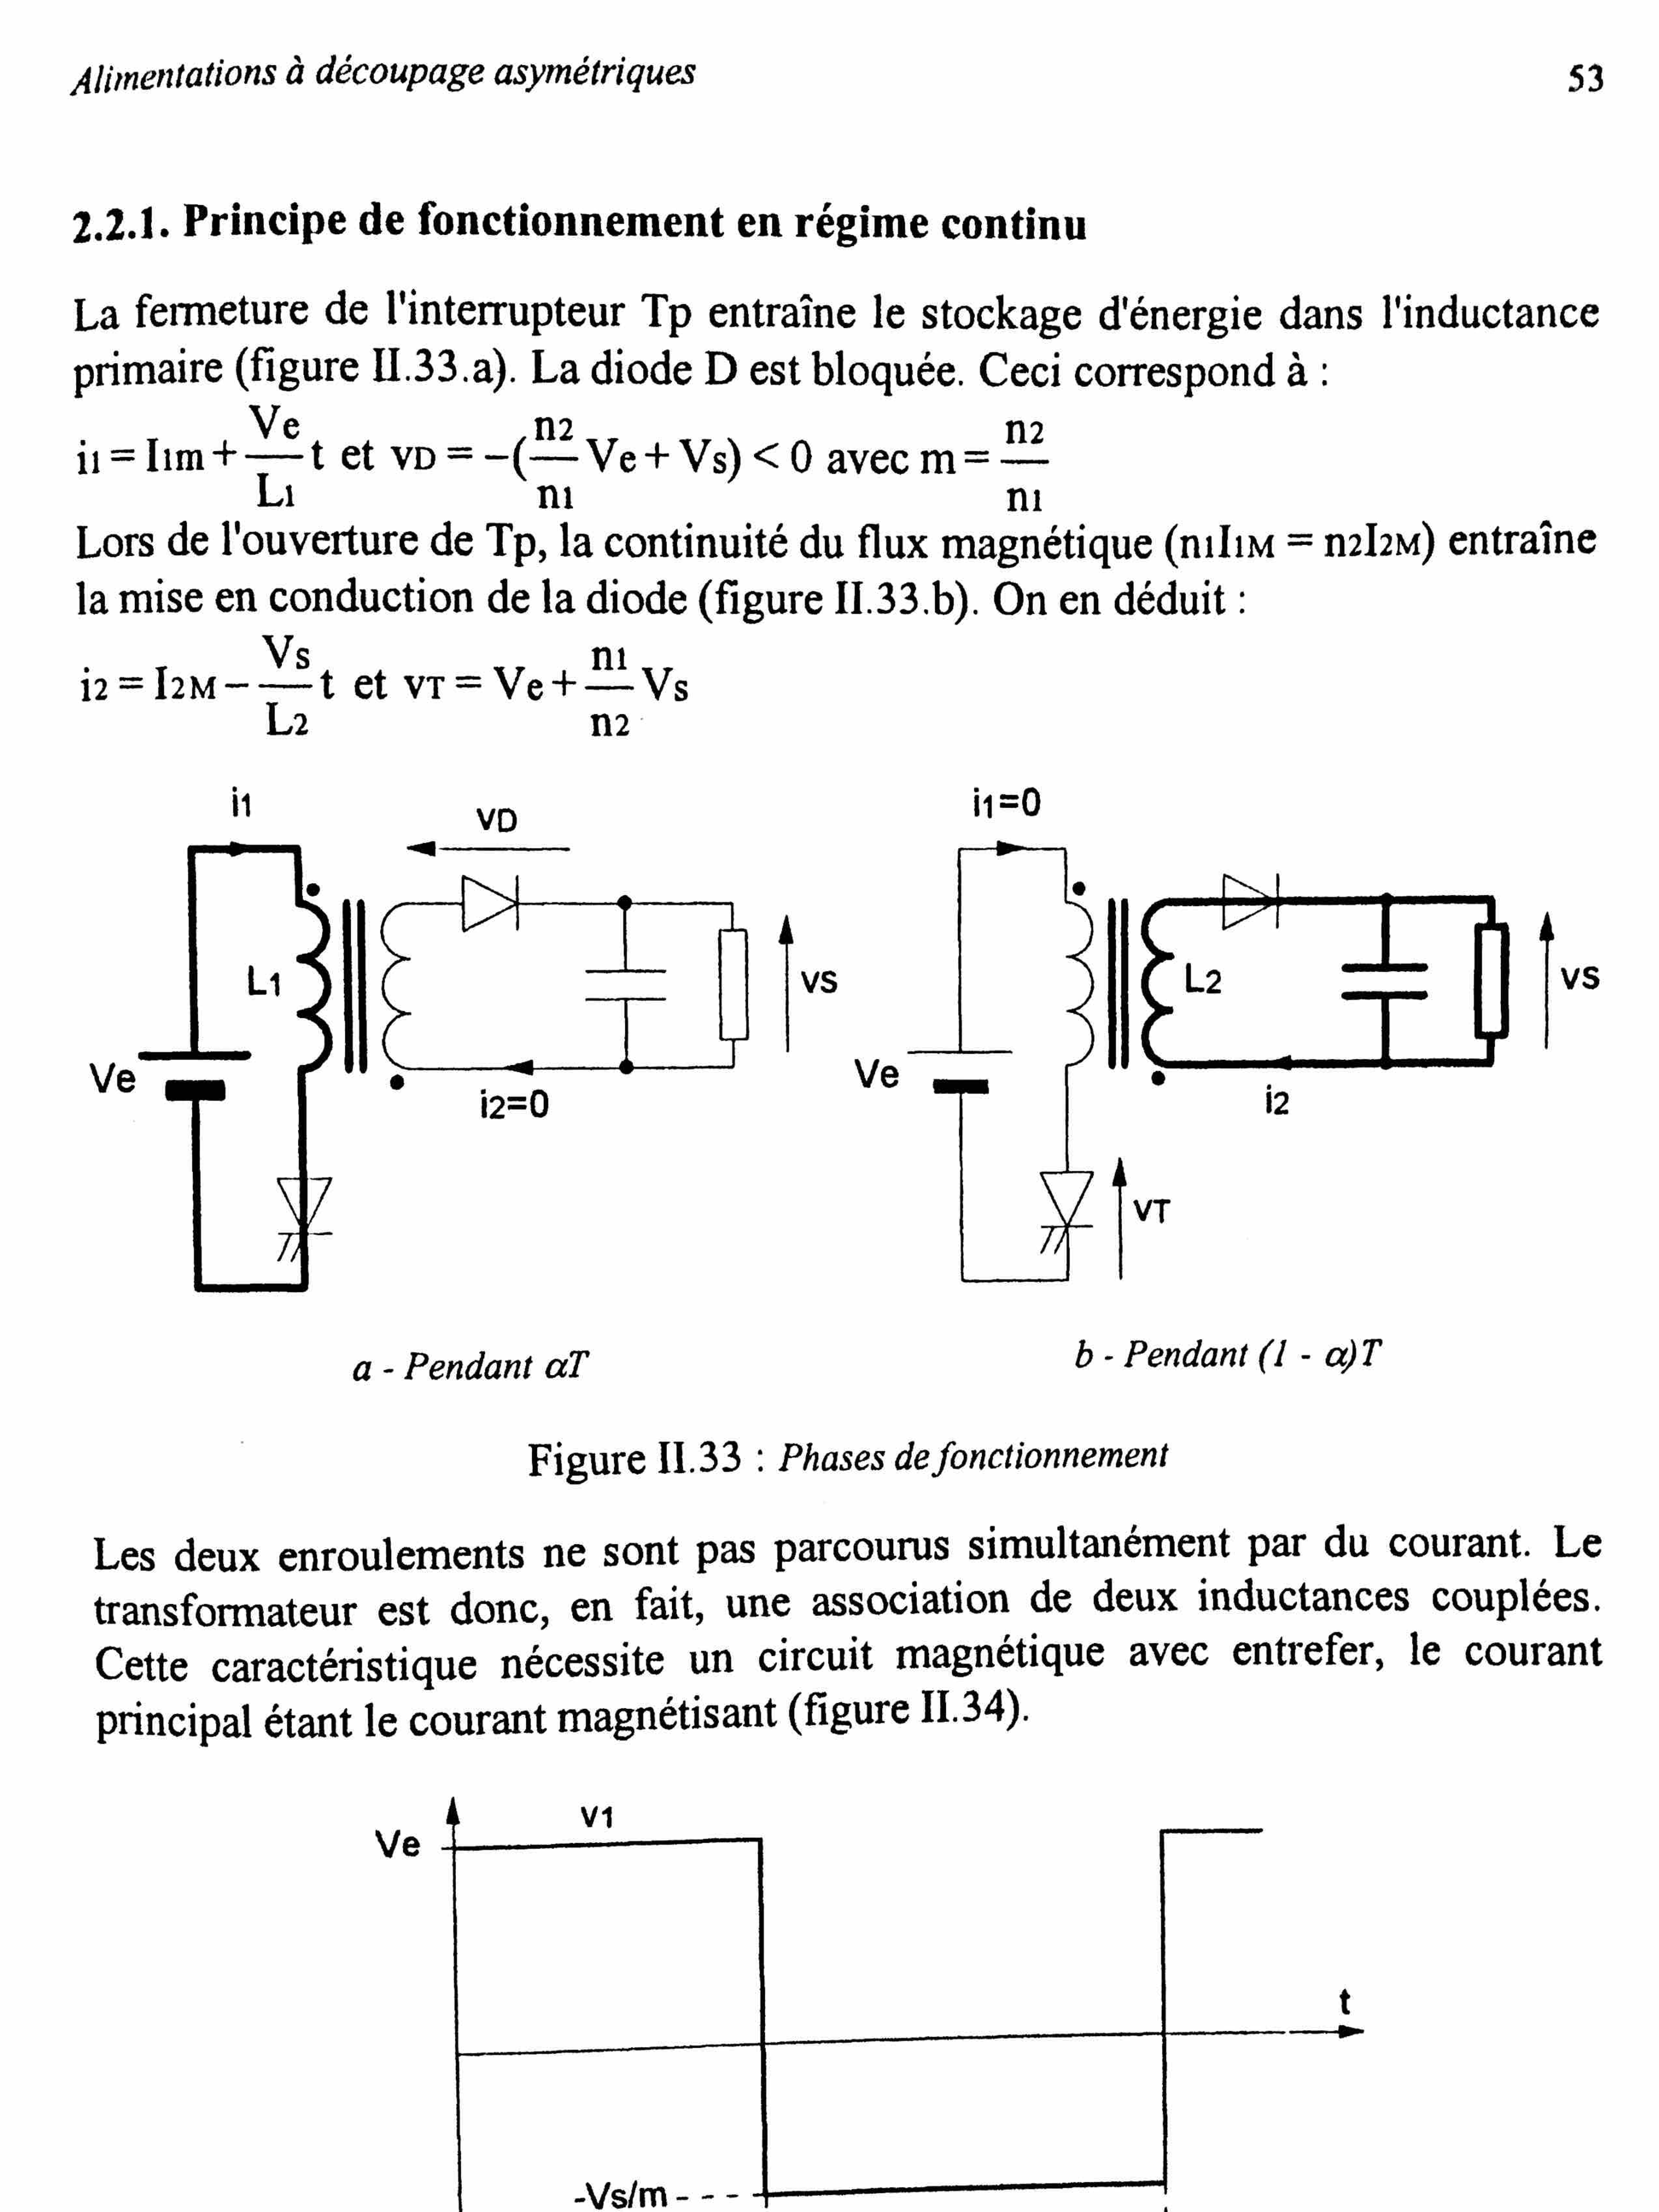
\includegraphics[width=6cm,trim=0cm 48cm 43.5cm 40cm, clip=true]{Images_Rapport/courants.pdf}
  \end{center}
  \vspace{-5pt}
  \caption{Fonctionnement durant $\alpha T_{dec}$}
  \vspace{-10pt}
\end{wrapfigure}
\vspace{30pt}
$V_1 = V_e $\par
\vspace{10pt}
$\phi (t) = \dfrac{V_e}{n_1}t + \phi_{min}$\par
\vspace{10pt}
$i_1 = \dfrac{V_e}{L_1} + i_{1min}$ 


\vspace{30pt}

\textbf{\underline{Pour t $\in$ [$\alpha T_{dec};T_{dec}$] : }}


\begin{wrapfigure}[2]{r}{0.5\textwidth}
  \vspace{-80pt}
  \hspace{-0pt}
  \begin{center}
    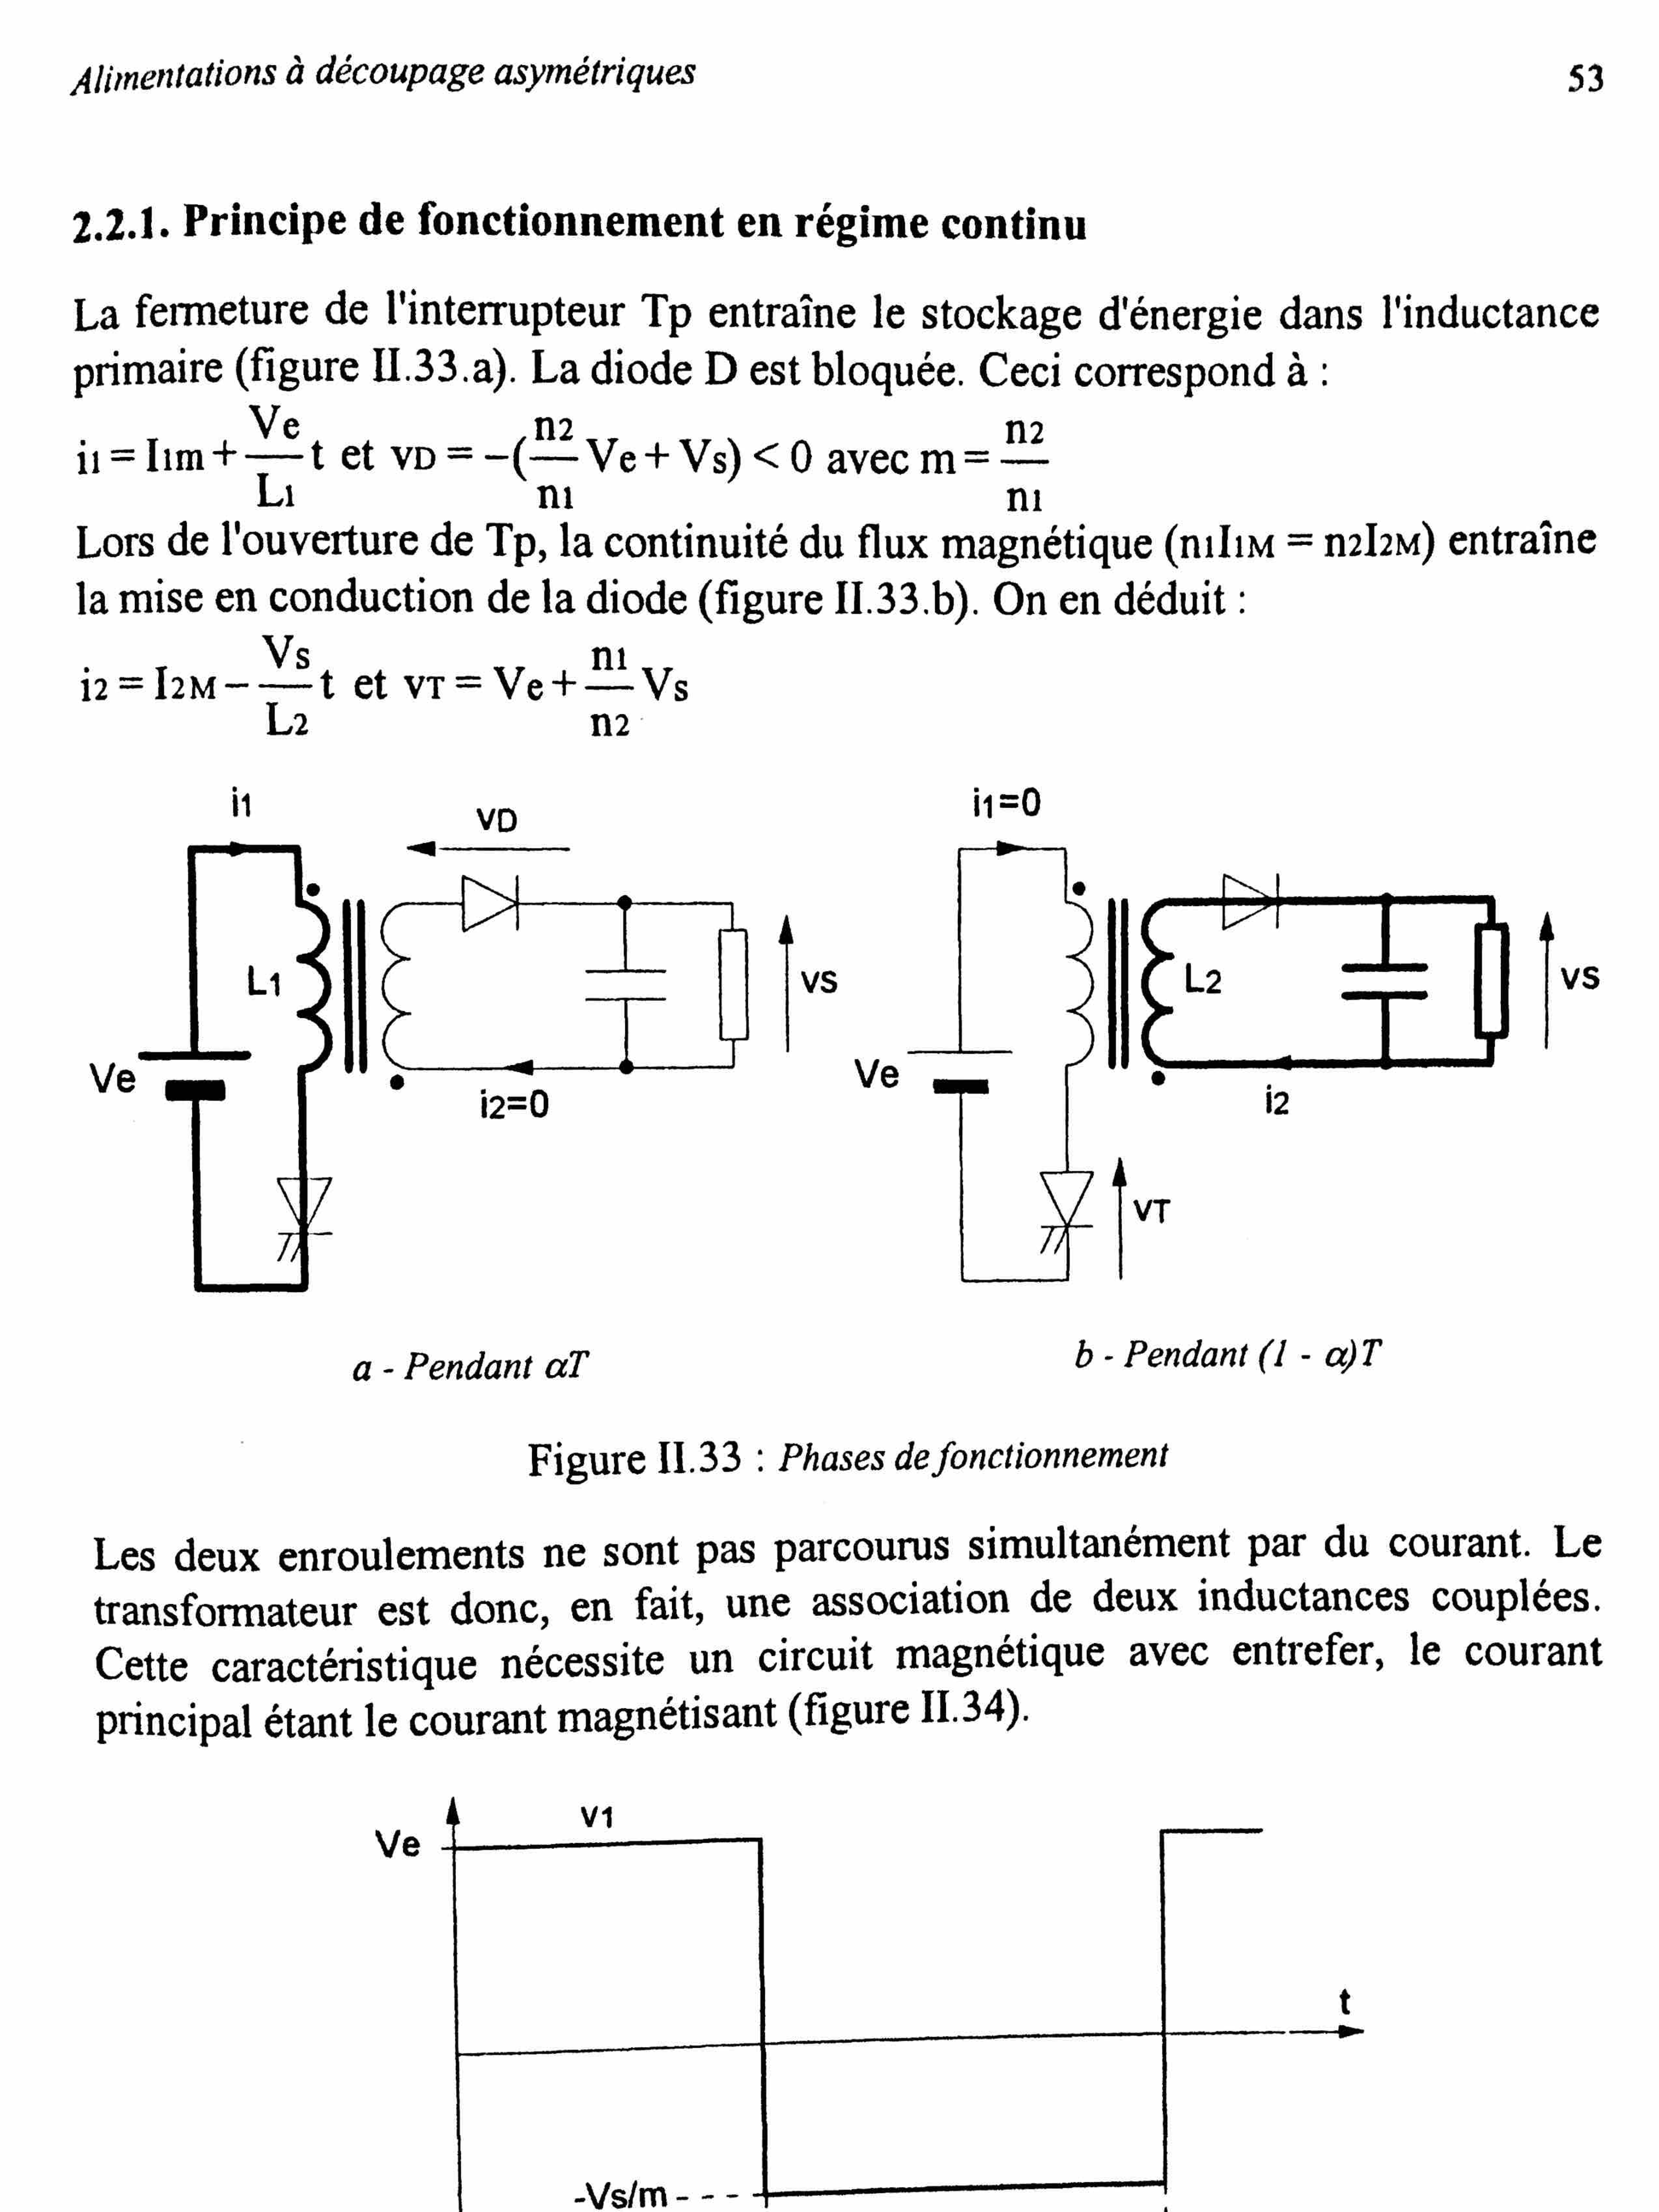
\includegraphics[width=6cm,trim=45.5cm 48cm 0cm 40cm, clip=true]{Images_Rapport/courants.pdf}
  \end{center}
  \vspace{-5pt}
  \caption{Durant $(1-\alpha). T_{dec}$}
  \vspace{-10pt}
\end{wrapfigure}


\vspace{20pt}
$\phi (t) = -\dfrac{V_s}{n_2}t + \phi_{max}$\par
\vspace{10pt}
$v_1 = n_1 \dfrac{d\phi}{dt} = -\dfrac{n_1}{n_2} V_s$ \par



\begin{wrapfigure}[3]{l}{0.5\textwidth}
  \vspace{-90pt}
  \hspace{-0pt}
  \begin{center}
    \fbox{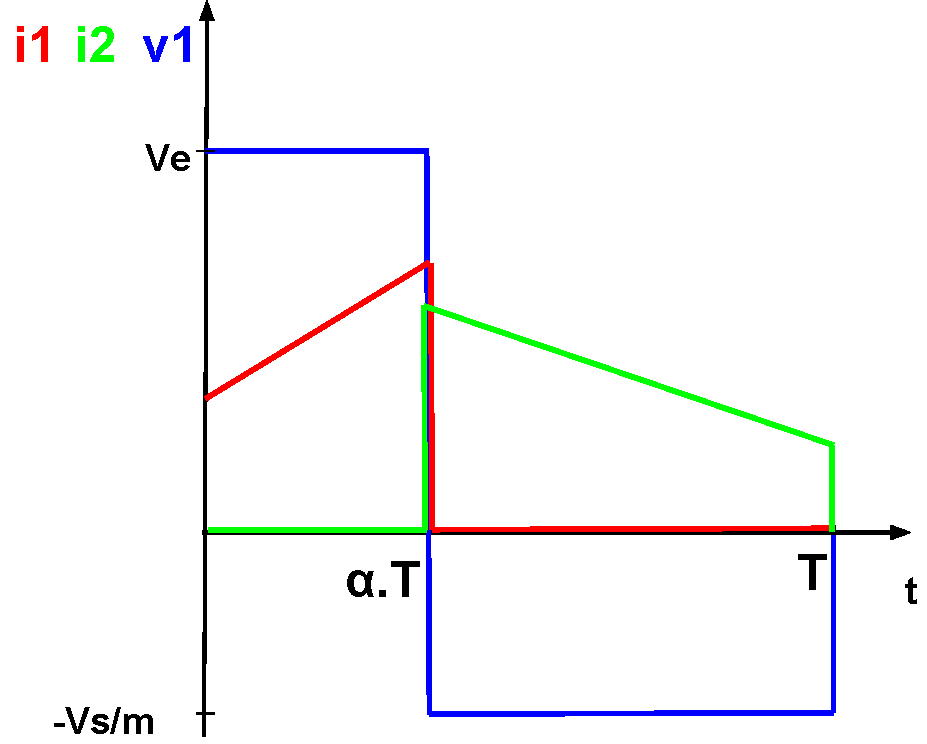
\includegraphics[width=7cm,trim=0cm 0cm 0cm 0cm, clip=true]{Images_Rapport/allures_flyback}}
  \end{center}
  \vspace{-5pt}
  \caption{Formes d'ondes idéales}
  \vspace{-10pt}
\end{wrapfigure}
\vspace{120pt}  
La figure ci-contre représente l'allure de l'évolution des courants dans $L_1$ et $L_2$ ainsi que de la tension aux bornes de $L_1$.  


\newpage
Ainsi en considérant que la valeur moyenne de la tension aux bornes de l'enroulement primaire se doit d'être nulle en régime établi sur une période de découpage il vient:\par
\vspace{10pt}

\[<v_1> = 0 \quad \Rightarrow \quad \dfrac{1}{T_{dec}}.(V_e .\alpha .T_{dec} - (1-\alpha) .T_{dec}.\dfrac{V_s}{m}) = 0 \quad \quad avec \quad \quad m = \dfrac{n_2}{n_1}\]


On en déduit la fonction de transfert statique du montage qui conditionnera l'ensemble du dimensionnement:\par
\vspace{10pt}

\begin{center}
\fbox{$\dfrac{V_s}{V_e} = \dfrac{m.\alpha}{1-\alpha}$}
\end{center}


\paragraph{Paramètres imposés}

Pour bien débuter le dimensionnement on s'impose plusieurs paramètres:\par
\vspace{10pt}

\begin{itemize}
\item La tension de sortie devra être de 18 V avec une ondulation maximale de 1$\%$.
\item La puissance du cahier des charges est de 18W mais on effectuera le dimensionnement pour $P_e$ = 22W en considérant 10\% de pertes en chutes de tension, un rendement des inductances d'environ 90\% et une petite marge de manoeuvre.
\item On se place toujours en démagnétisation incomplète afin de minimiser le volume des inductances.
\item On effectue le dimensionnement pour $\alpha = 0,5$. La marge de manoeuvre permettant de fonctionner autour de 0,4 lorsque la structure demandera 18W. 
\item Le bus d'entrée est supposé être le réseau domestique français parfaitement redressé soit $V_e = $325 V. 
\item La fréquence de découpage est choisie égale à 50 kHz.
\end{itemize}

\vspace{10pt}

%\begin{figure}[!h]
%  \hspace{-60pt}
%  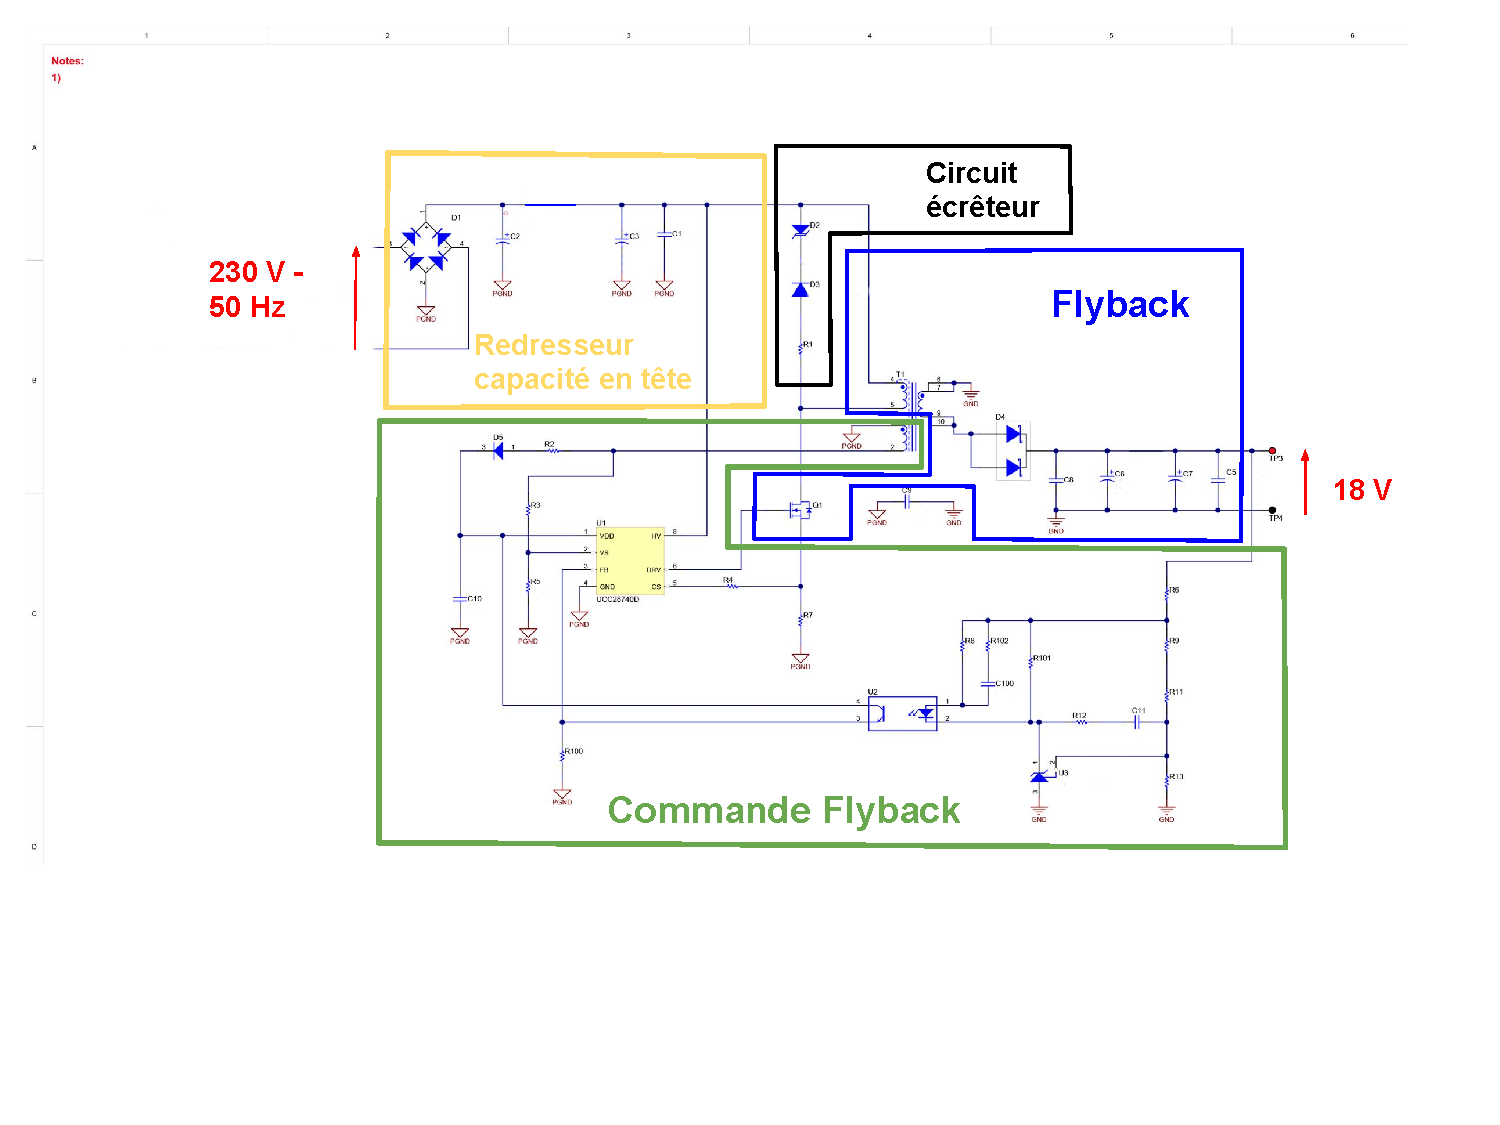
\includegraphics[width=21cm,trim=3cm 4cm 0cm 2cm, clip=true]{Images_Rapport/complet}
%  
%  
%  \caption{Structure générale d'un convertisseur Flyback}
%  
%\end{figure}



\paragraph{Calcul des inductances couplées}

Les inductances couplées étant l'élément central de la structure, elles méritent une attention particulière pour assurer le bon fonctionnement général. 


En partant des conditions imposées et de la fonction de transfert statique on commence par calculer le rapport de transformation m :\par


\vspace{5pt}

$$\dfrac{V_s}{V_e} = \dfrac{m.\alpha}{1-\alpha} \quad \Rightarrow \quad m = \dfrac{V_s}{V_e}.\dfrac{1-\alpha}{\alpha} = \dfrac{18}{325}.\dfrac{1-0.5}{0.5} \quad \Rightarrow \quad \fbox{m=  0,055}$$

\vspace{15pt}
Ensuite en se plaçant en limite de conduction continue (le flux s'annule précisement en fin de période) l'énergie à emmagasiner dans l'inductance primaire donne la valeur de celle-ci:



$$W_e = \frac{1}{2}L_1 I_{1max}^2 \quad\Rightarrow\quad P_e = \frac{1}{2}L_1 I_{1max}^2F_{dec} \quad \Rightarrow \quad P_e = \frac{1}{2}L_1(\dfrac{V_e\alpha T_{dec}}{L_1})^2F_{dec} \quad \Rightarrow \quad \fbox{$L_1$ = 12 mH}$$

De plus d'après le modèle du transformateur parfait on a : \fbox{$L_2 = L_1.m^2 = 36 \mu H$}\par
\vspace{10pt}

La suite du dimensionnement est réalisée à l'aide d'un algorithme \cite{labible} dont les résultats sont présentés dans le tableau ci-dessous.

\vspace{15pt}
\hspace{-80pt}
\begin{tabular}{|>{\bf}l|c|c|} \hline
Paramètre & \textbf{Critère de dimensionnement} & \textbf{Choix} \\ \hline
Densités de courants  & Arbitraire $\in$ [0;10] A.$mm^{-2}$ & J = 5 $A.mm^{-2}$\\\hline Courant efficaces enroulements & $i_{1eff} = \dfrac{V_e}{\sqrt{24}L_1F_{dec}}$ \quad $i_{2eff} = \dfrac{V_s}{\sqrt{24}L_2F_{dec}}$  &$i_{1eff} = 0,11 $A \par  $i_{2eff} = 2,04$A\\ \hline
Diamètres conducteurs & $\dfrac{i}{J} = S = \dfrac{\pi d^2}{4}$ &  $d_1 = 0,17 mm$ \quad $d_2 = 0,72mm$\\\hline
Nature des conducteurs & Epaisseur de peau $\delta p = \sqrt{\dfrac{2}{\omega\mu \sigma}}$ = 0,3 mm &  Monobrins\\\hline
Coefficients de bobinage & $\dfrac{S_{carre}}{S_{cercle \quad inscit}}$ & $k_b =  \dfrac{4}{\pi}$\\\hline
Induction maximale & $B_M < B_{sat}$ & $B_M = 200$ mT\\\hline
Produit des aires & $A_i = S_f.S_b = \dfrac{L_1.I_{1max}}{n_1.B_M}.\sum_{j=1}^N\dfrac{k_{bj}.n_j.i_{jeff}}{J_j} $ & $A_i = 1,39.10^{-9} m^4$ mT\\\hline
Circuit magnétique & $A_{i-reel} \geq A_{i-calcul}$ & Pot RM-10\\\hline
Surfaces réelles & Lecture datasheet & $S_f = 83 mm^2$\quad $S_b = 41,5 mm^2$\\\hline
Nombre de spires & $n_1 = \dfrac{L_1I_{1max}}{B_MS_f} = \dfrac{n_2}{m}$ & $n_1 = 199 $\quad $n_2 = 11$\\\hline
Entrefer & $e = \dfrac{\mu_0n_1^2S_f}{L_1}$ & $e = 0,35 $ mm\\\hline



\end{tabular}


\vspace{10pt}

Les images de la réalisation pratique de ce transformateur sont données ci-dessous:\par
\vspace{15pt}




\begin{figure}[!h]
  \hspace{-30pt}
  \vspace{-30pt}
  \begin{minipage}[b]{0.45\linewidth}
   \centering
   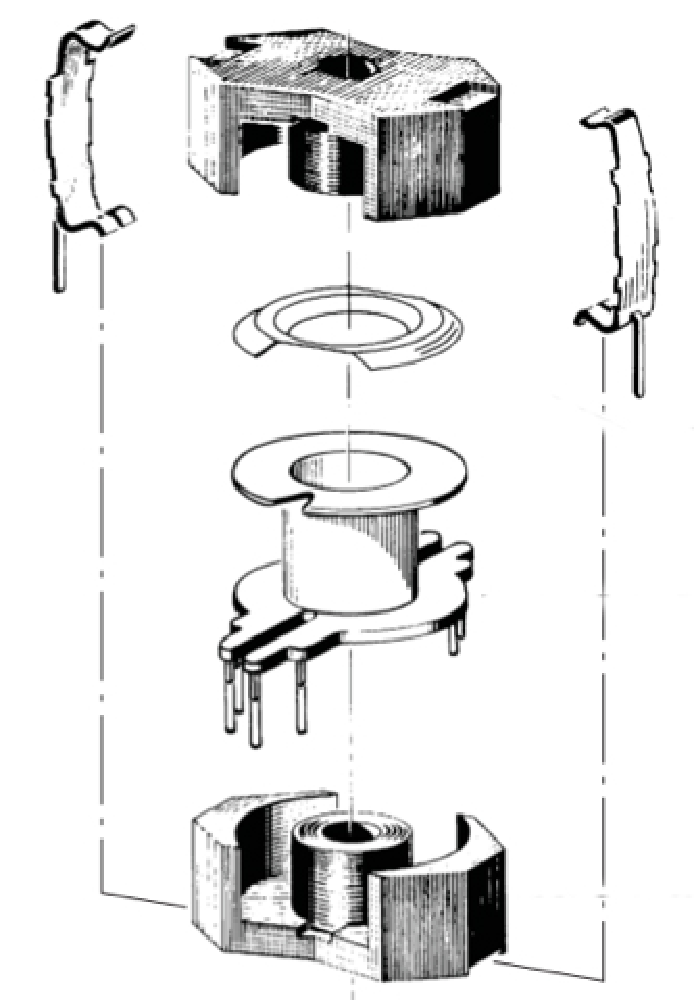
\includegraphics[width=7cm,height=5cm,trim=0cm 0cm 0cm 0cm, clip=true]{Images_rapport/pot}  
   \caption{Pot RM-10}   
  \end{minipage}
\hfill
  \begin{minipage}[b]{0.45\linewidth}
   \centering
   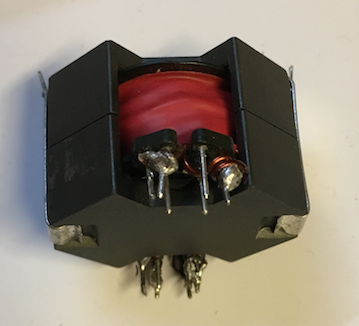
\includegraphics[width=7cm,height=5cm,trim=0cm 0cm 0cm 0cm, clip=true]{Images_rapport/transfo}  
   \caption{Inductances couplées}   
  \end{minipage}
\end{figure}

\vspace{15pt}

\begin{figure}[!h]
  \hspace{-30pt}
  \vspace{-30pt}
  \begin{minipage}[b]{0.45\linewidth}
   \centering
   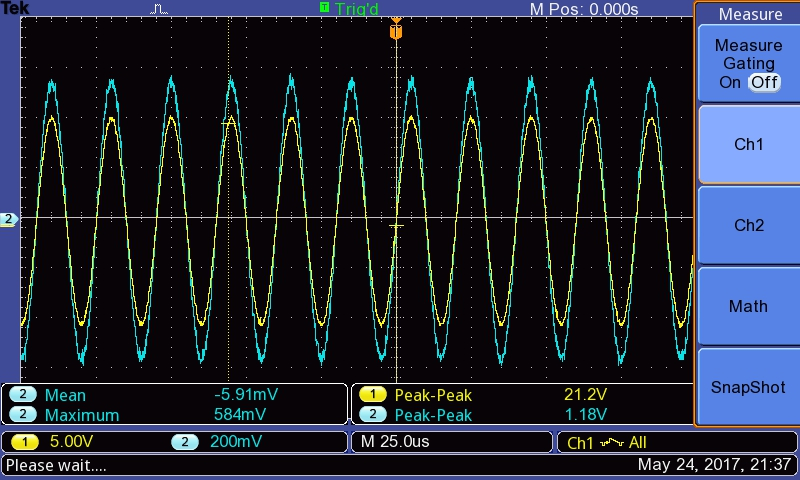
\includegraphics[width=7cm,height=5cm,trim=0cm 0cm 0cm 0cm, clip=true]{Images_rapport/Transfo2}  
   \caption{Rapport de transformation}   
  \end{minipage}
\hfill
%  \begin{minipage}[b]{0.45\linewidth}
%   \centering
%   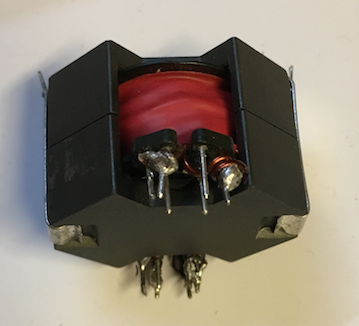
\includegraphics[width=7cm,height=5cm,trim=0cm 0cm 0cm 0cm, clip=true]{Images_rapport/transfo}  
%   \caption{Inductance de fuites}   
%  \end{minipage}
\end{figure}
\vspace{40pt}






















\newpage
\paragraph{Essais de simulation}

Afin de vérifier les calculs précédents ainsi que la faisabilité de la structure il est possible de la simuler entièrement avec l'aide de l'outil Simscape de Matlab®. Le schéma de la structure réalisée est présenté figure 28.

\begin{figure}[!h]
  \hspace{-60pt}
  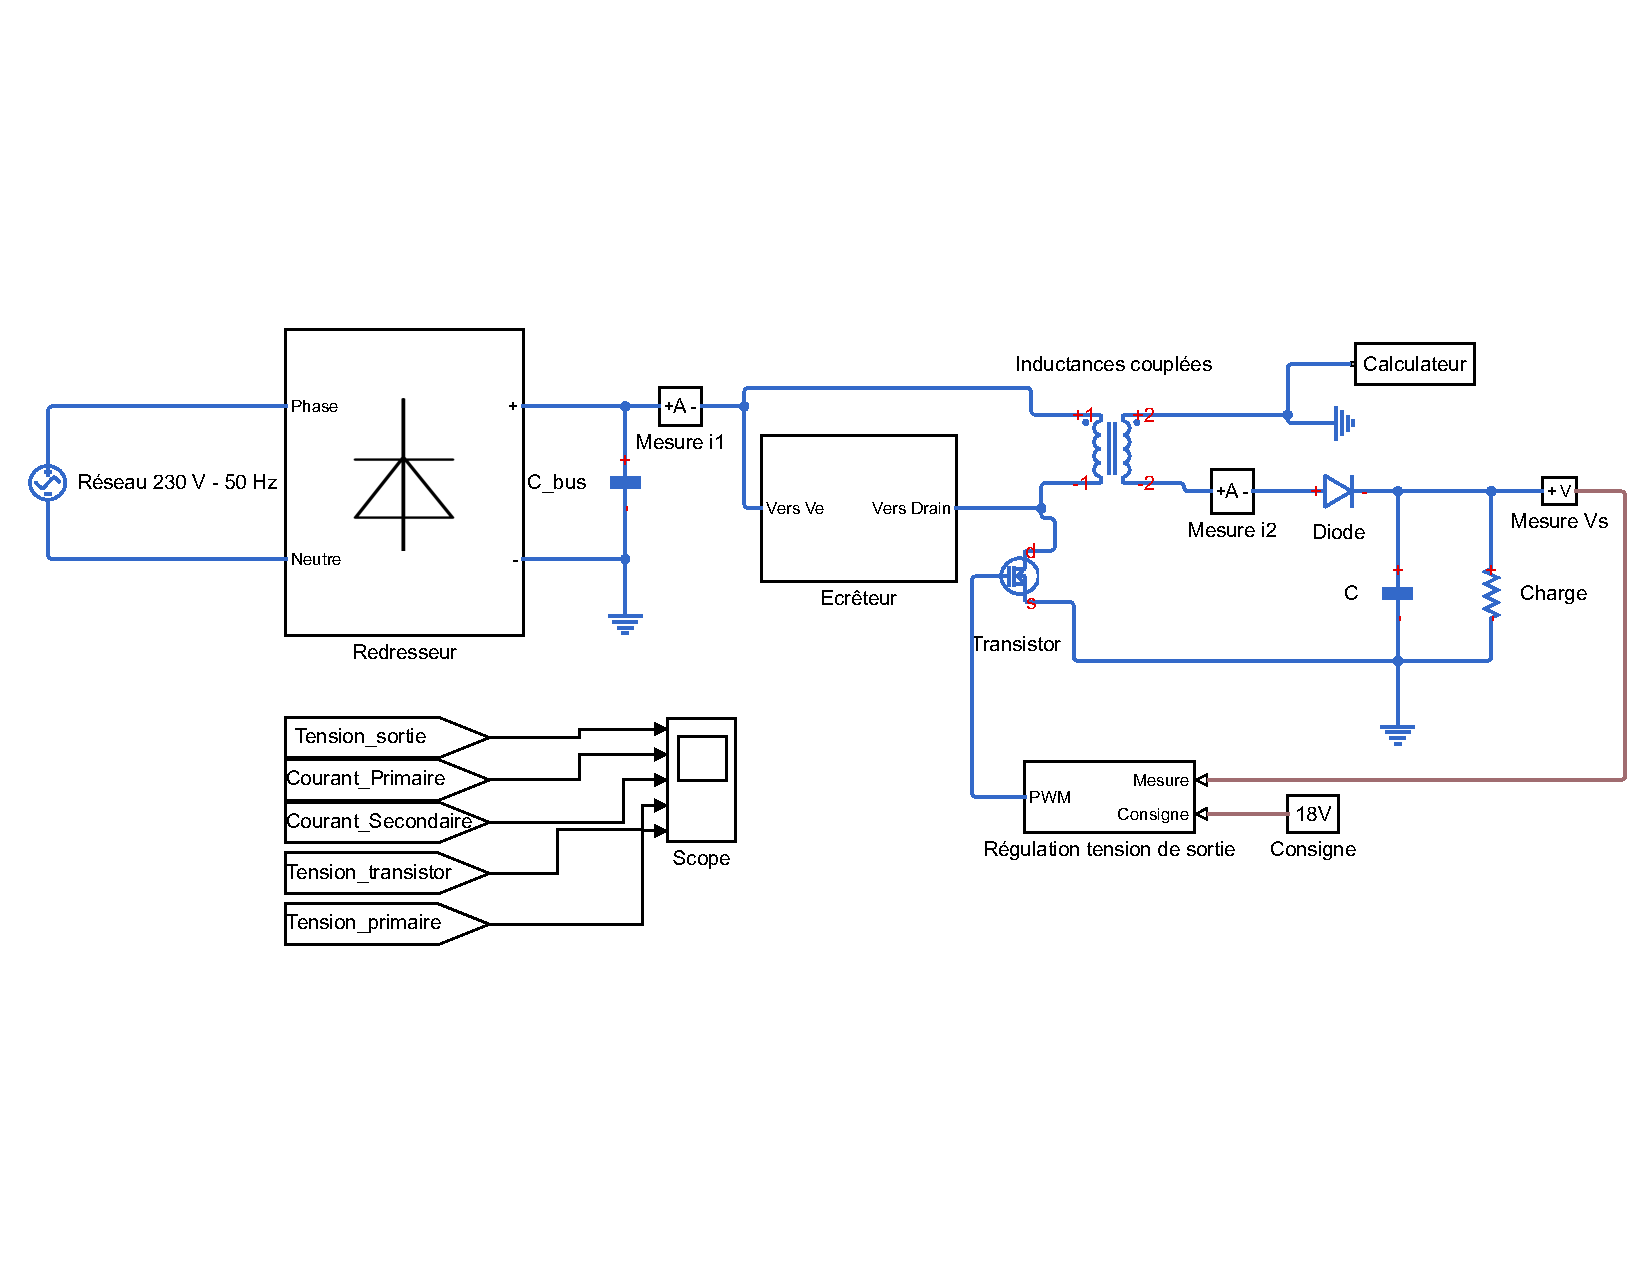
\includegraphics[width=20cm,trim=0cm 5cm 0cm 5cm, clip=true]{Images_Rapport/flyback_simscape}
  
  
  \caption{Modélisation Simscape du convertisseur }
  
\end{figure}

Sur ce modèle on distingue la structure générale de l'alimentation Flyback ainsi que le redresseur à diodes capacité en tête et le réseau précédemment cités. Les inductances sont paramétrées avec les valeurs issues des calculs précédents auxquels il est possible d'ajouter la prise en compte de fuites magnétiques.\par 
Deux blocs supplémentaires essentiels au bon fonctionnement sont également présents: un bloc de commande permettant de réguler la tension de sortie à la valeur souhaitée et un bloc d'écrêtage permettant de diminuer les contraintes en tension subies par le transistor.\par 

\vspace{10pt}
\begin{figure}[!h]
  \hspace{-30pt}
  \vspace{-30pt}
  \begin{minipage}[b]{0.45\linewidth}
   \centering
   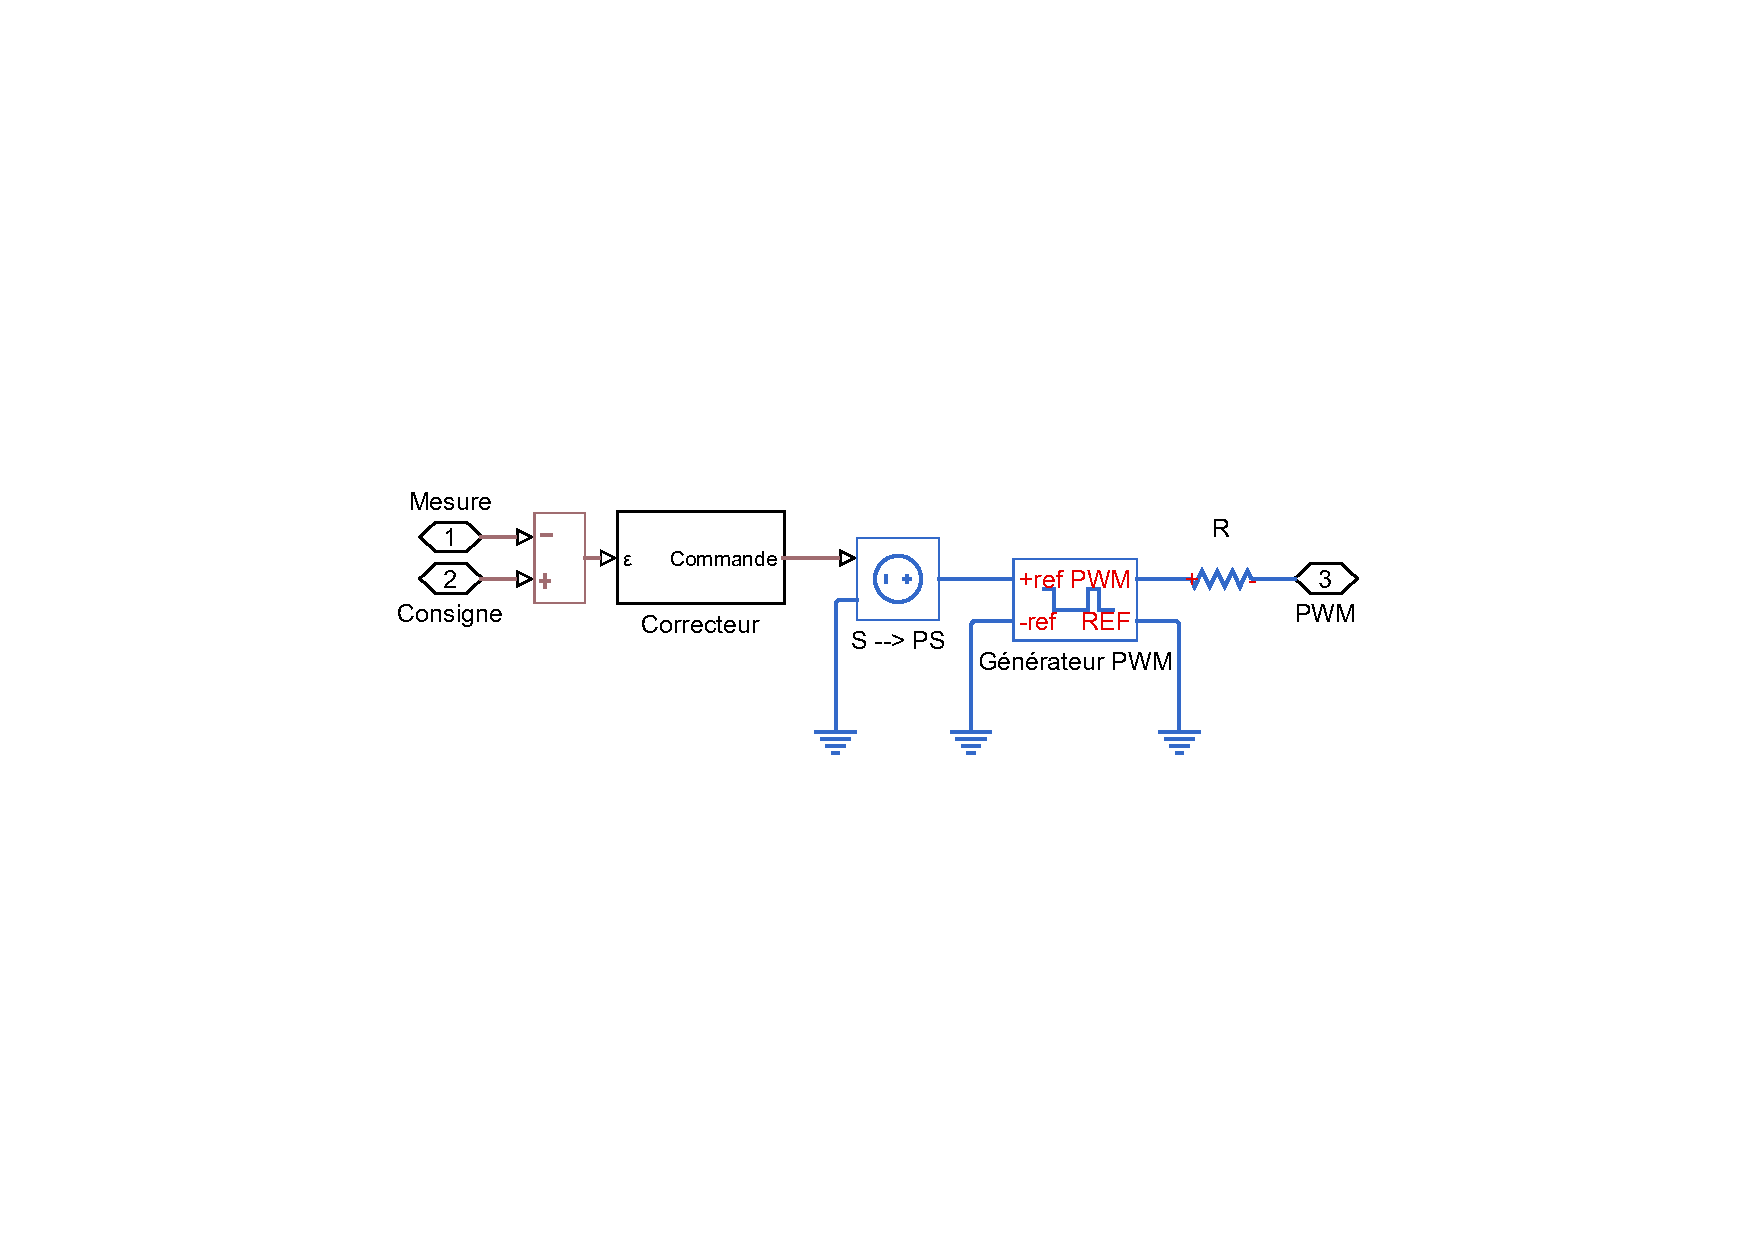
\includegraphics[width=9cm,trim=6cm 7cm 6cm 7cm, clip=true]{Images_rapport/commande}  
   \caption{Circuit de commande}   
  \end{minipage}
\hfill
  \begin{minipage}[b]{0.45\linewidth}
   \centering
   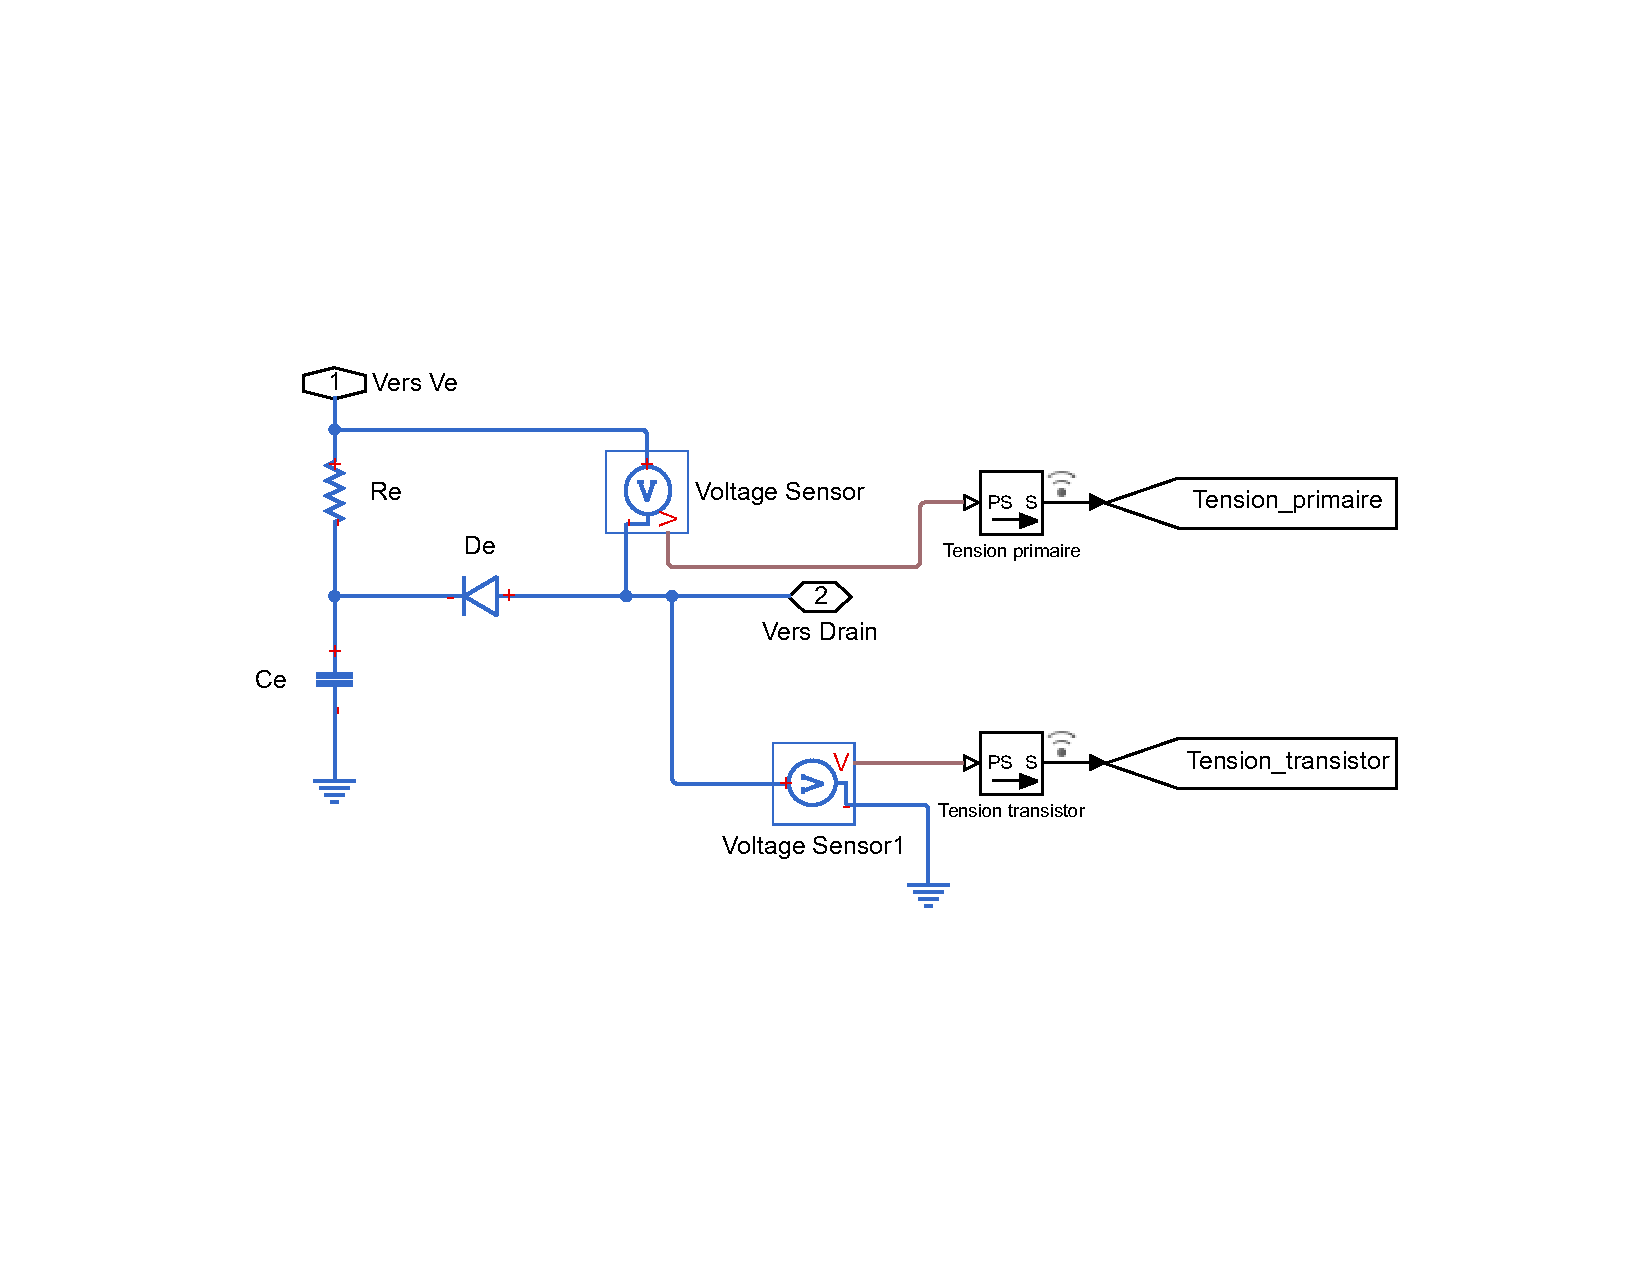
\includegraphics[width=9cm,trim=4cm 6cm 4cm 6cm, clip=true]{Images_rapport/ecreteur}  
   \caption{Circuit écrêteur}   
  \end{minipage}
\end{figure}

\vspace{10pt}
\newpage
\textbf{Le circuit de commande} permet de maintenir la tension de sortie à la consigne de 18V par comparaison et correction proportionnelle intégrale. La commande ainsi élaborée permet de générer un signal PWM controlant l'ouverture et la fermeture du transistor.\par 
\vspace{10pt}

\textbf{Le circuit écrêteur  } permet de protéger le transistor des imperfections des inductances couplées. En effet le couplage n'étant pas parfait il existe des fuites magnétiques. Il est alors possible de modéliser ces fuites par une inductance $l_{fp}$. Cette inductance emmagasine de l'énergie qu'il faut libérer à chaque période de découpage. Le circuit écrêteur permet de dissiper cette énergie sans appliquer de fortes surtensions au transistor.

 
\begin{figure}[!h]
  \centering
  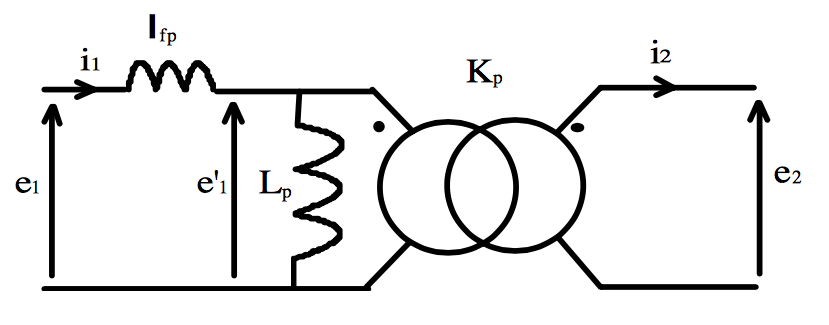
\includegraphics[width=8cm,height = 3cm,trim=0cm 0cm 0cm 0cm, clip=true]{Images_Rapport/multon}
  
  
  \caption{Modèle du transformateur avec fuites au primaire \cite{Multon}}
  
\end{figure}

\vspace{15pt}

Les résultats obtenus avec ce modèle sont les suivants : 
 
 
\begin{figure}[!h]
\hspace{-40pt}
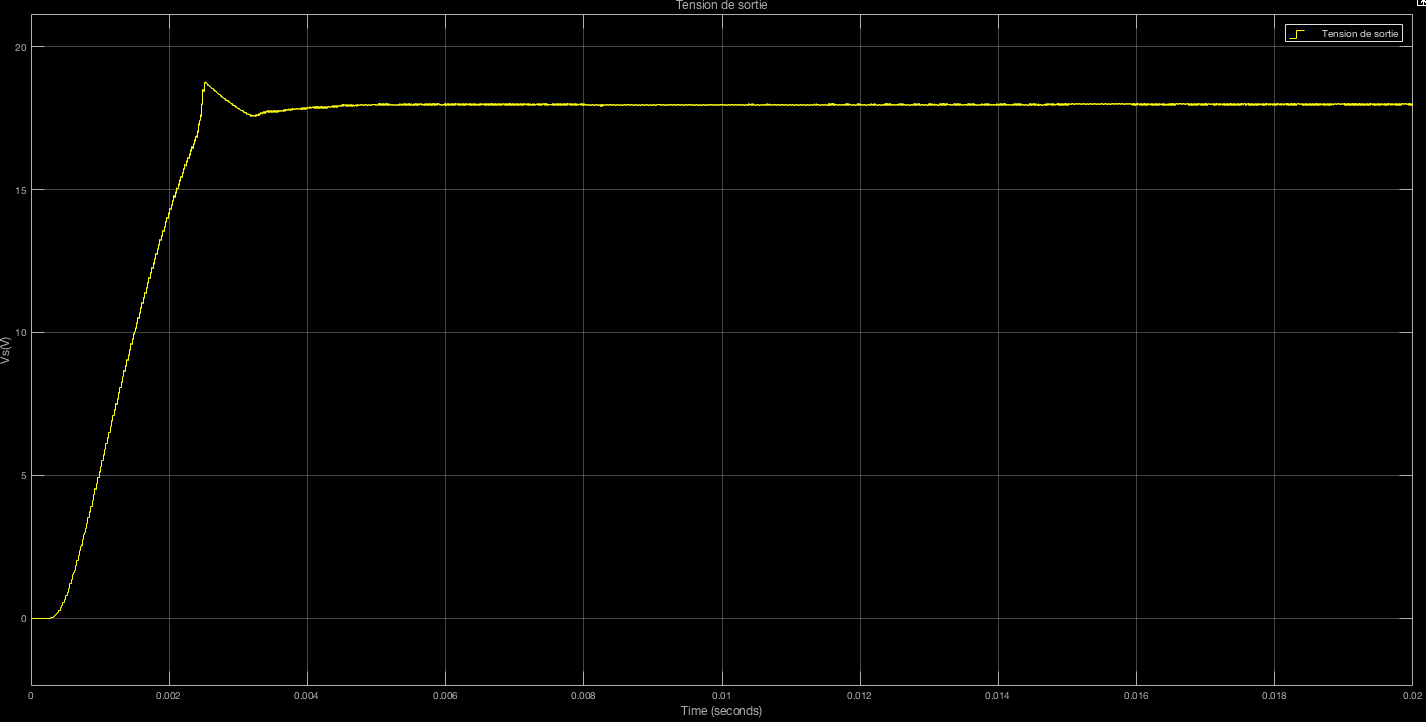
\includegraphics[width=19cm,height = 5cm,trim=0cm 0cm 0cm 0cm, clip=true]{Images_Rapport/t}
\caption{Allure de la tension de sortie au démarrage}
\end{figure}
 
\vspace{10pt} 
\begin{figure}[!h]
\hspace{-40pt}

\includegraphics[width=19cm,height = 5cm,trim=0cm 0cm 0cm 0cm, clip=true]{Images_Rapport/c}
\caption{Allures des courants dans les enroulements}
\end{figure}  
  \vspace{10pt}
  
Si les allures générales semblent satisfaisantes il est également intéressant de zoomer afin de voir si on retrouve bien les formes d'onde attendues.  
  
  
 \vspace{5pt}
 
% \begin{figure}[!h]
%\centering
%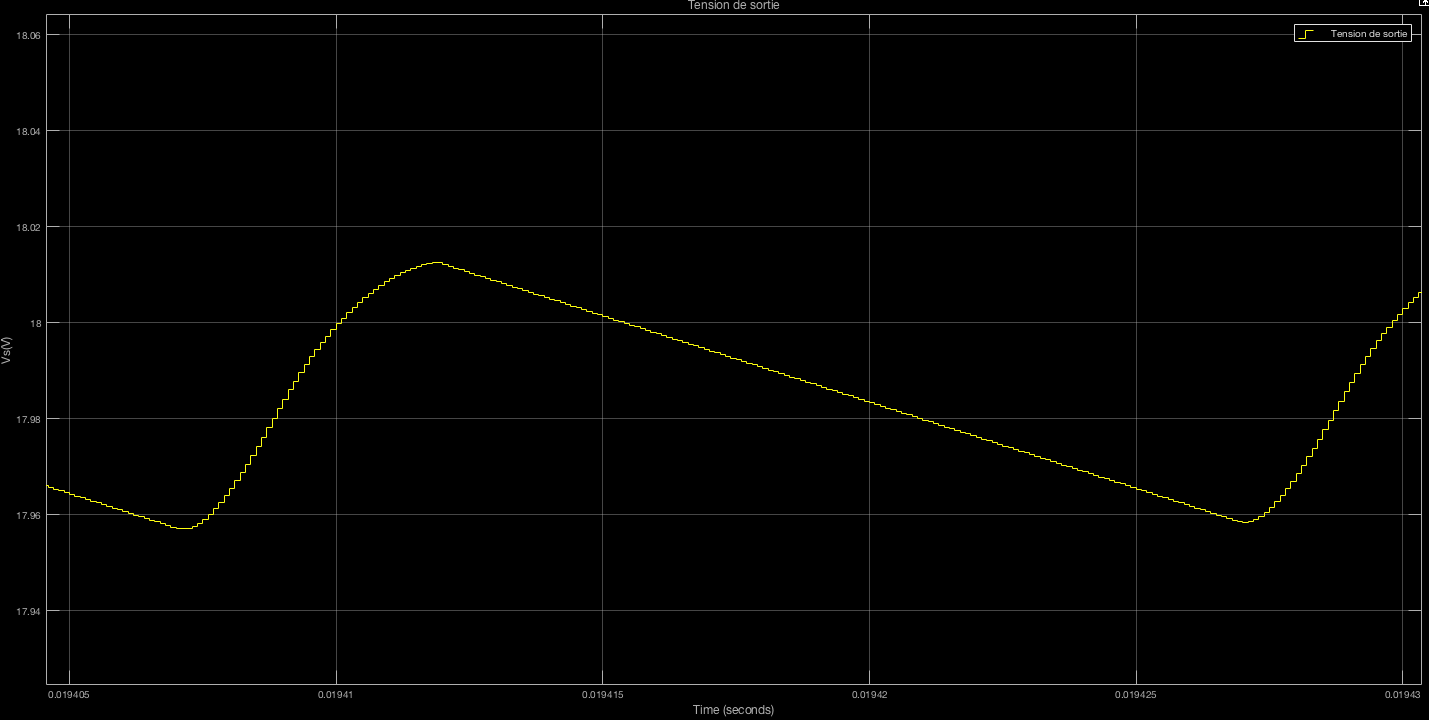
\includegraphics[width=12cm,height=6cm,trim=0cm 0cm 0cm 0cm, clip=true]{Images_Rapport/ot}
%\caption{Ondulations de la tension de sortie}
%\end{figure}
%
%\begin{figure}[!h]
%\centering
%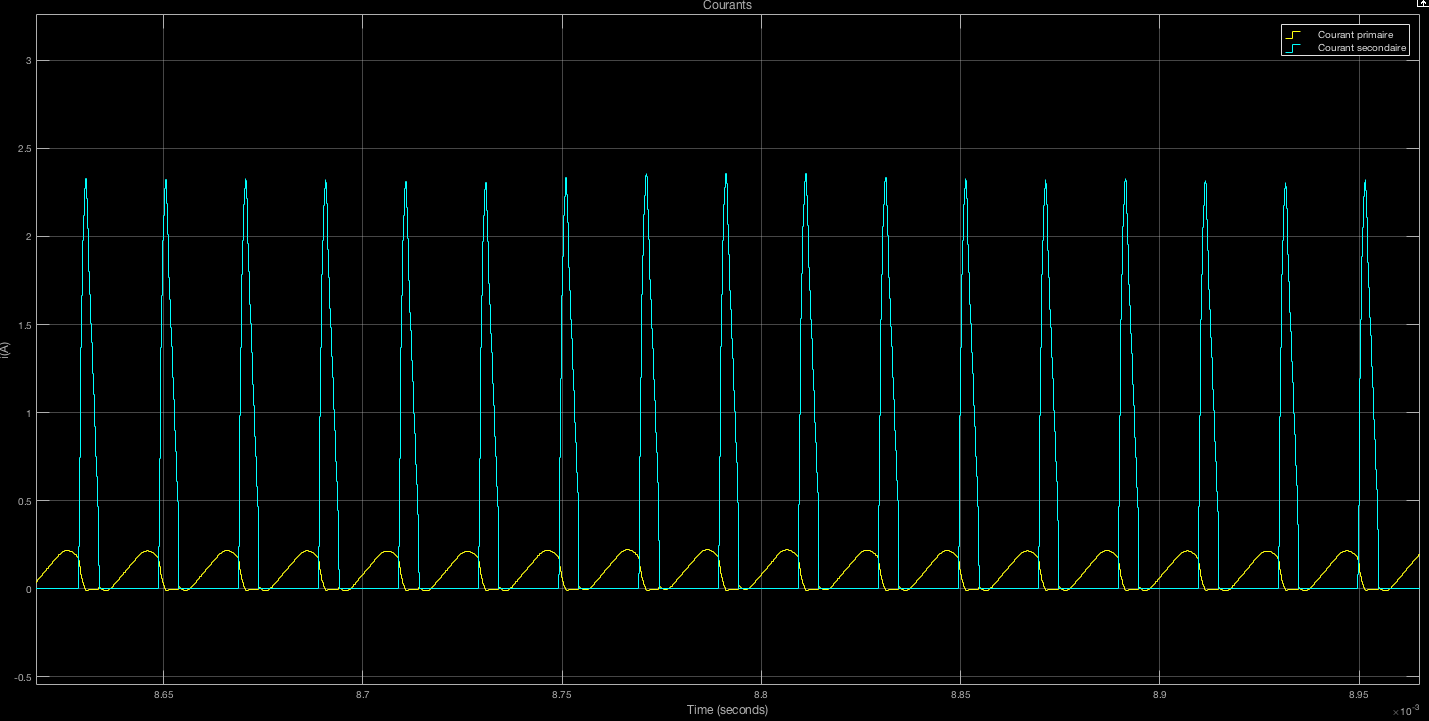
\includegraphics[width=12cm,height=6cm,trim=0cm 0cm 0cm 0cm, clip=true]{Images_Rapport/oc}
%\caption{Ondulations de courant dans les enroulements}
%\end{figure}
\begin{figure}[!h]
  \hspace{-30pt}
  \vspace{-30pt}
  \begin{minipage}[b]{0.5\linewidth}
 
   \hspace{-20pt}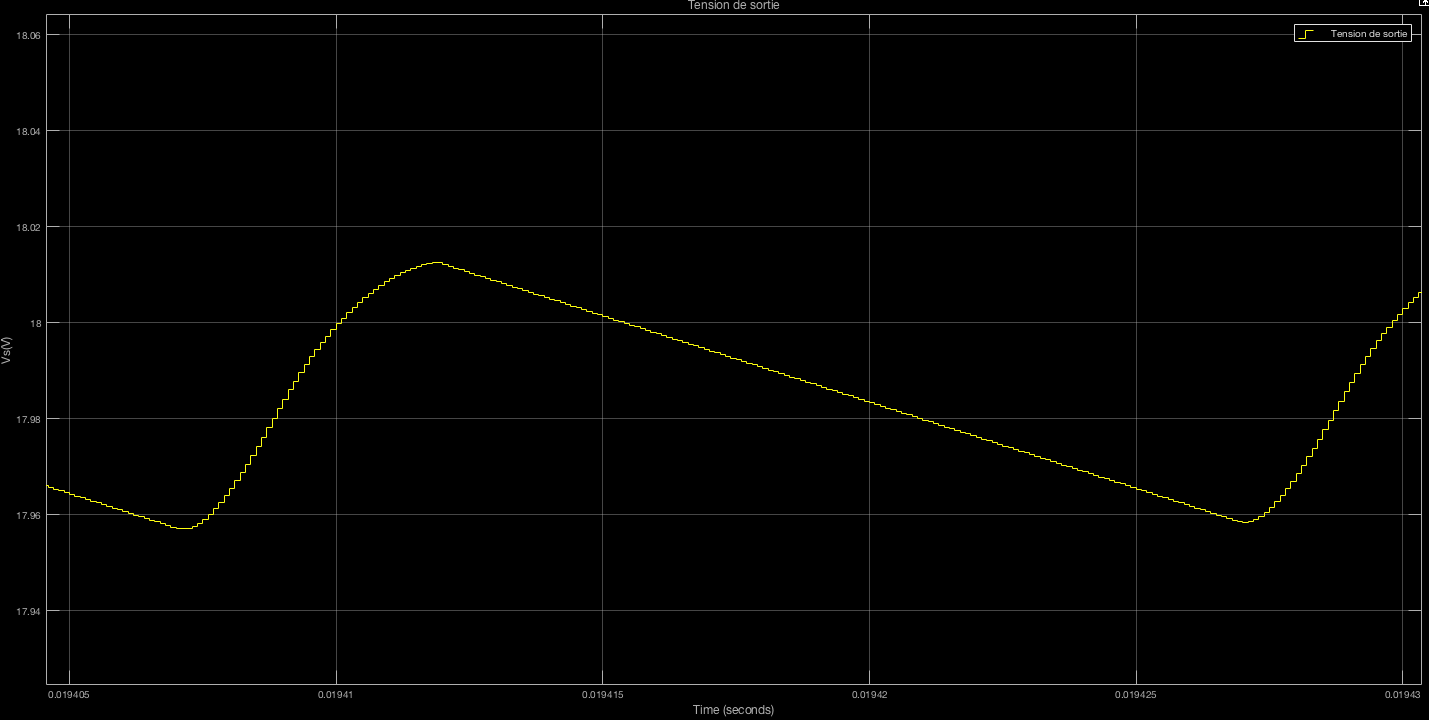
\includegraphics[width=9.5cm,height = 6cm,trim=0cm 0cm 0cm 0cm, clip=true]{Images_rapport/ot}  
   \caption{Ondulations tension de sortie}   
  \end{minipage}
\hfill
  \begin{minipage}[b]{0.5\linewidth}
   \hspace{5pt}
   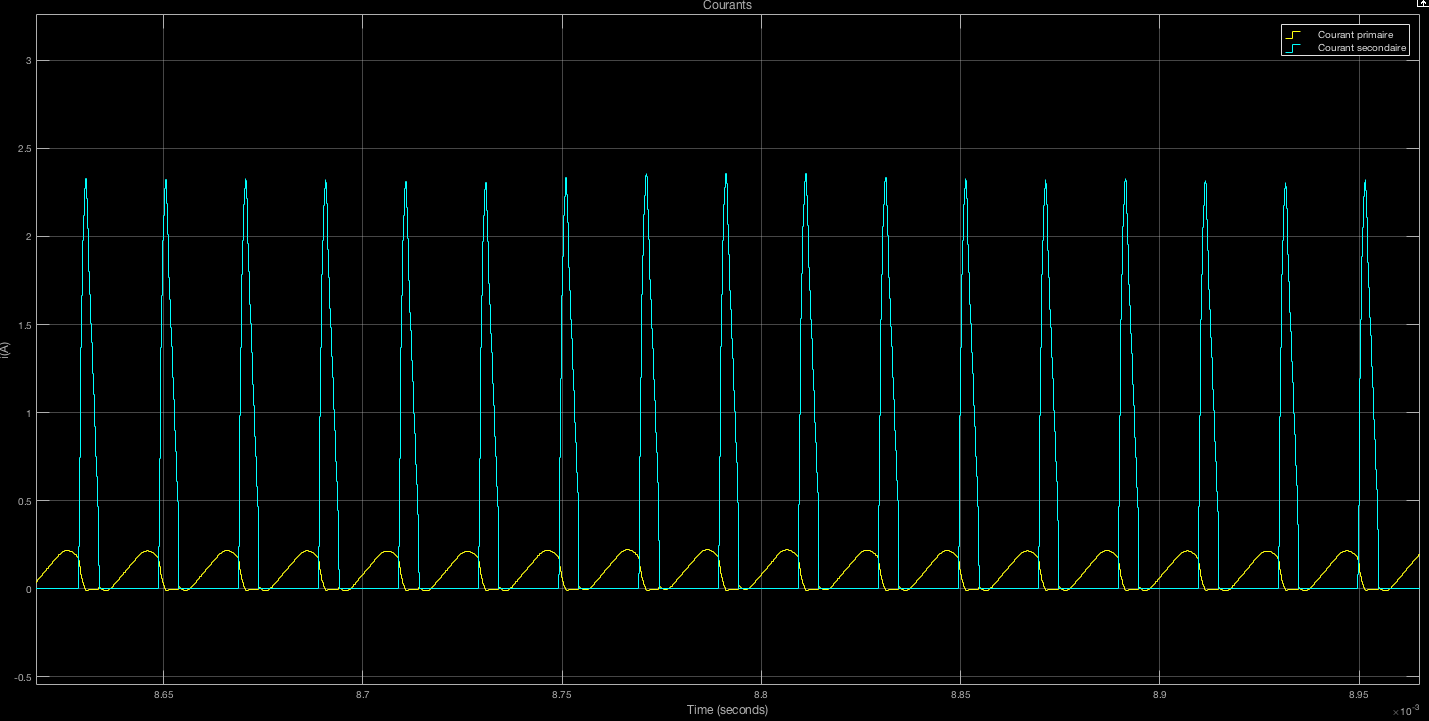
\includegraphics[width=9.5cm,height = 6cm,trim=0cm 0cm 0cm 0cm, clip=true]{Images_rapport/oc}  
   \caption{Ondulations de courant}   
  \end{minipage}
\end{figure}
 
\vspace{20pt}

\paragraph{Système réel}
 
Le systèe réel finalement choisit est en tout point identique au système simulé à l'exception faite du circuit de commande. Celle-ci est en effet basée sur une puce Texas Instruments UCC28740 qui à partir d'une image de la tension de sortie obtenue via un optocoupleur gère l'ouverture et la fermeture du transistor.\par


\vspace{5pt}

\subsection{Conclusion de la partie scientifique} 
 
Ma collaboration avec echOpen m'a dans un premier temps permis d'étudier le fonctionnement d'un appareil d'échographie portable qui sera sans nul doute une future aide précieuse pour améliorer le diagnostic de miliers de personnes dans le monde et ainsi diminuer le taux de mortalité évitable. Dans un second temps j'ai été amené à participer encore plus activement au projet puisque j'ai pu mettre à profit mes connaissances sur les convertisseurs de puissance dans le but d'apporter une proposition de solution rendant le système effectivement plus mobile et ainsi plus proche que jamais de remplir son cahier des charges complet. \par 
\vspace{8pt}
Les deux parties de mon travail au cours de cette collaboration étant relativement différentes cela m'offre une certain richesse scientifique qu'il m'est possible de mettre à profit dans la suite de ce dossier en proposant deux applications pédagogiques possibles relatives à chacune d'elles.
 
 
 
 
 
 
 
  
\newpage

\newpage





\newpage
\section{Seconde partie: Approches pédagogiques}

\subsection{Exploitation pédagogique en première STI2D spécialité SIN}

\subsubsection{Contexte}

La filière STI2D (Sciences et Technologies de l'Industrie et du Développement Durable) est née en 2011 de la réforme des baccalauréats technologiques qui faisait suite à une baisse importante des effectifs de la filière STI.

\begin{wrapfigure}[11]{r}{0.5\textwidth}
  \vspace{-10pt}
  \hspace{-0pt}
  \begin{center}
    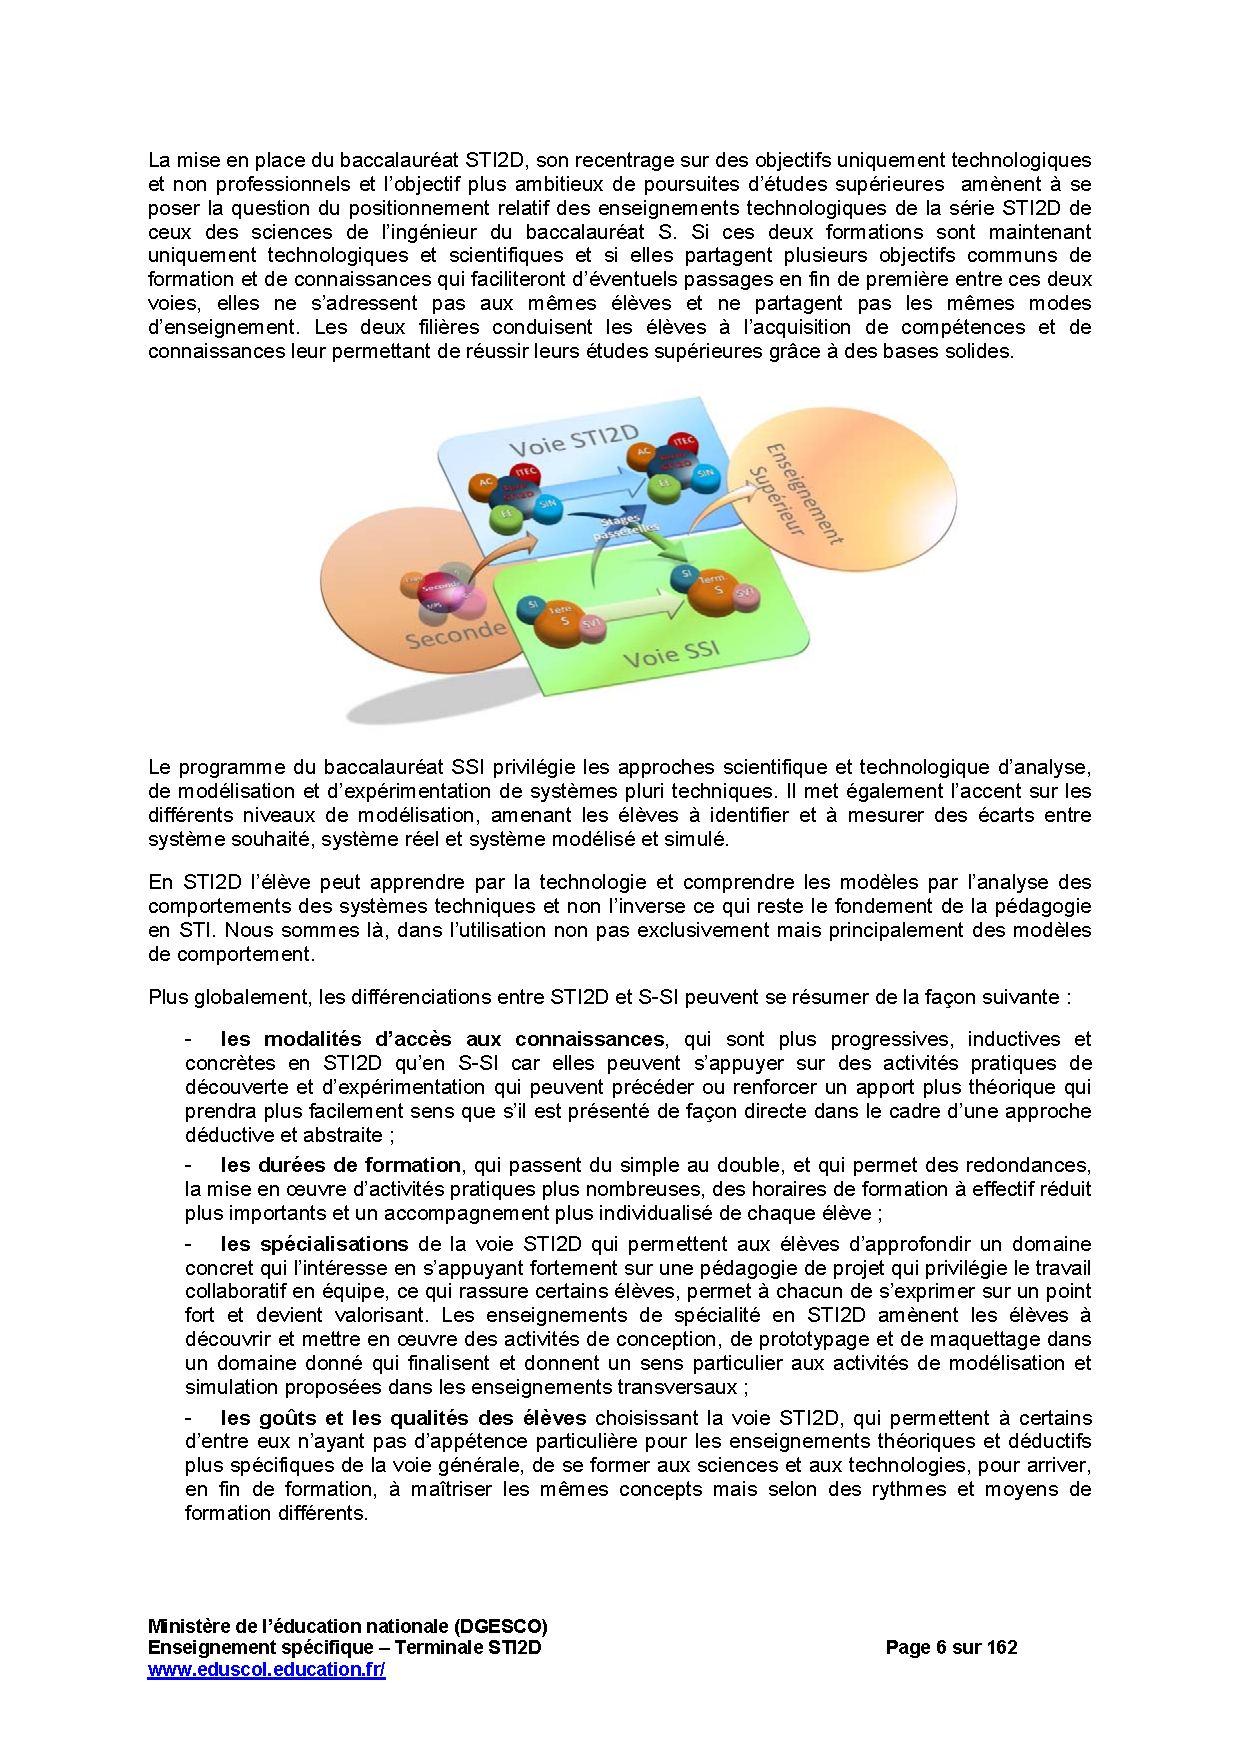
\includegraphics[width=6cm,height=4cm,trim=5cm 17.5cm 4.5cm 6.5cm, clip=true]{Images_Rapport/poursuite_etude}
  \end{center}
  \vspace{-5pt}
  \caption{Placement de la filière STI2D}
  \vspace{-10pt}
\end{wrapfigure}
\vspace{20pt}
Si l'enjeu des filières technologiques à longtemps été d'amener les élèves vers une formation post-baccalauréat courte (type S.T.S. ou I.U.T) la donne a aujourd'hui changé. La filière STI2D est devenue un parallèle à la filière générale scientifique. La filière STI2D vise une formation par la technologie et la démarche inductive mais ce n'est plus une filière professionnalisante et l'objectif est aujourd'hui de permettre aux élèves de s'engager dans des études supérieures longues type école d'ingénieur.\par
\vspace{20pt}

Afin de renforcer cette volonté d'apprentissage par la technologie et d'arriver à amener les élèves à acquérir les connaissances et compétences nécessaires à leurs études futures la voie STI2D s'est dotée de 4 spécialisations. Cela permet aux élèves d'approfondir dans un domaine concret qui les intéressent, les rassurent et les valorisent notamment via le travail de projet en équipes.\par
\vspace{20pt}


\begin{wrapfigure}[8]{r}{0.5\textwidth}
  \vspace{-50pt}
  \hspace{-0pt}
  \begin{center}
    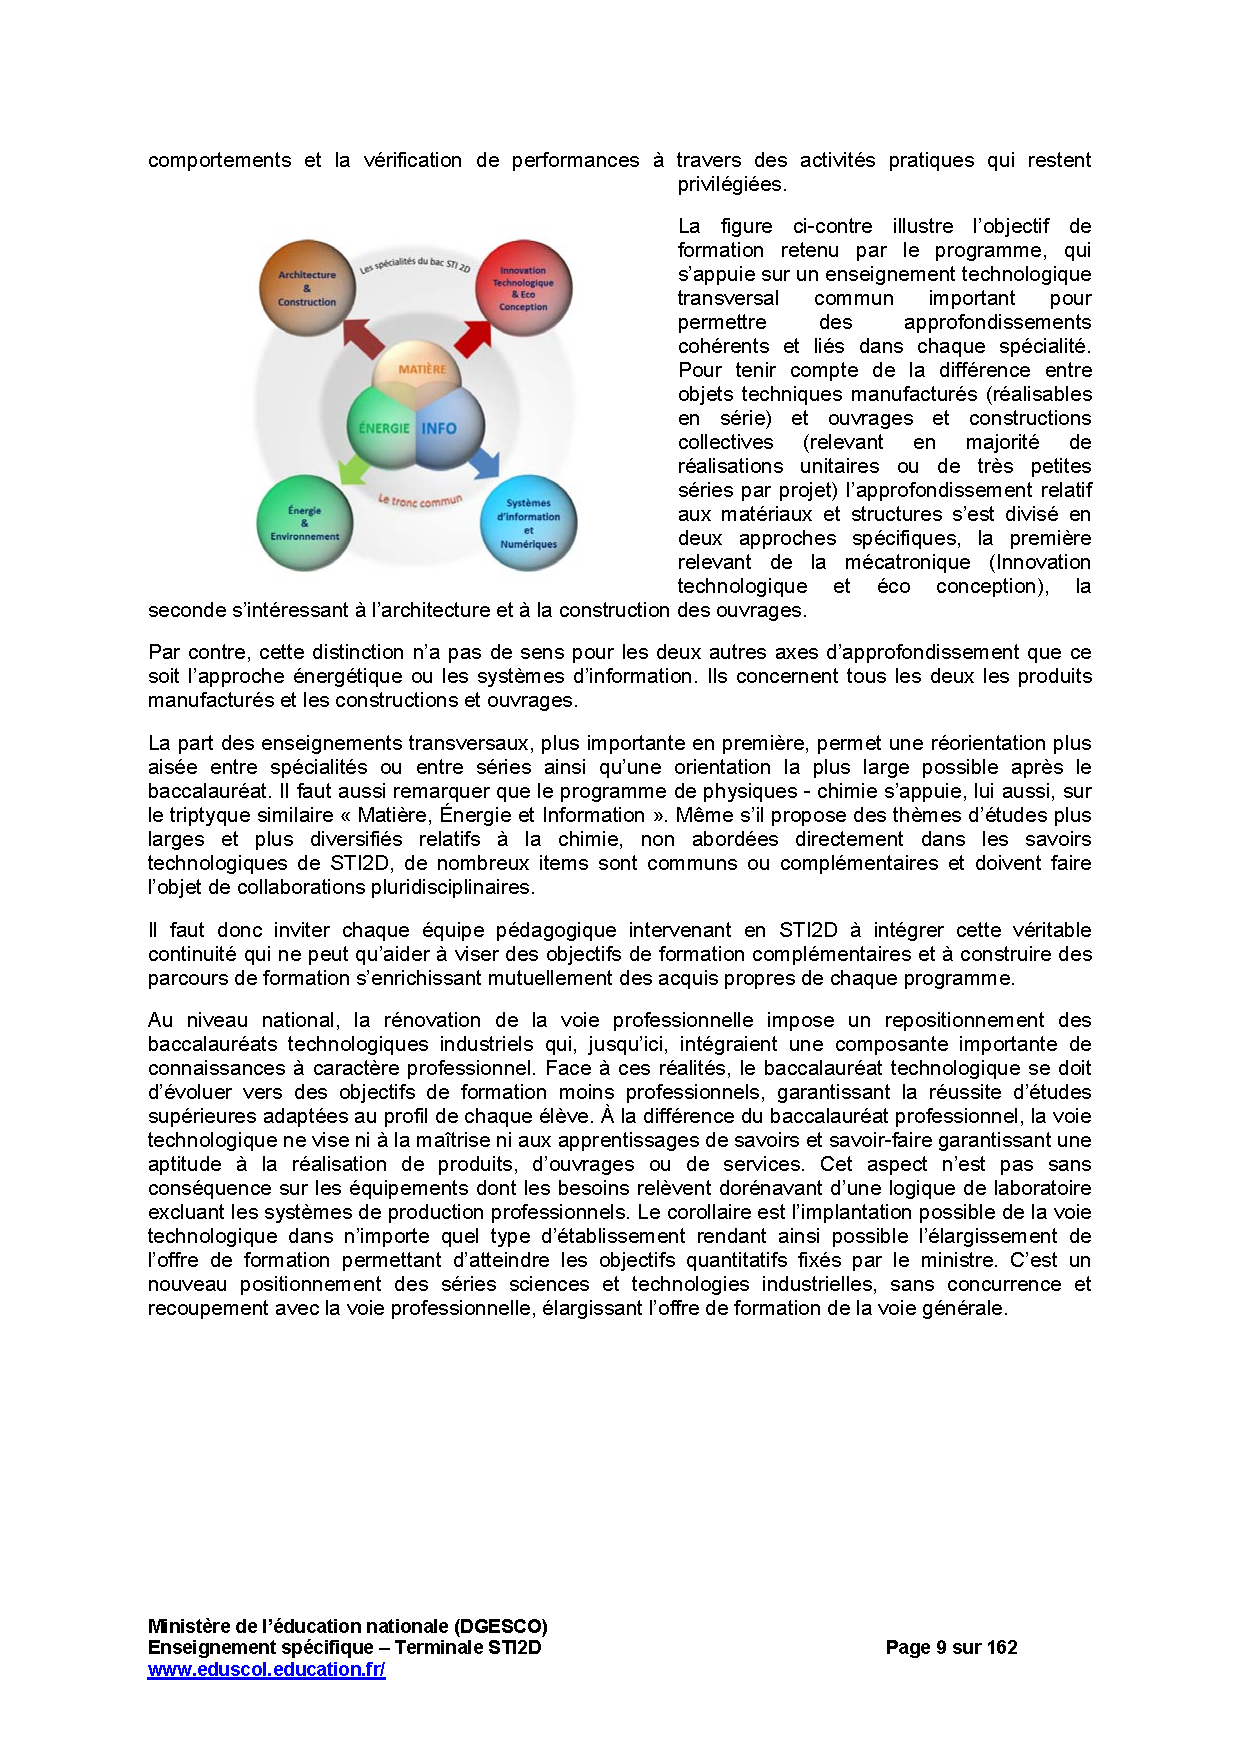
\includegraphics[width=8cm,height=5cm,trim=3cm 19.8cm 10cm 3.3cm, clip=true]{Images_Rapport/specialite}
  \end{center}
  \vspace{-5pt}
  \caption{Spécialités en STI2D}
  \vspace{-10pt}
\end{wrapfigure}

\vspace{30pt}
La spécialité qui m'intéresse pour cette application pédagogique est la spécialité Système d'information et numérique (SIN). Cette spécialité propose dans le prolongement de ce qui est étudié dans l'enseignement transversal de faire l'étude de système pluri-techniques intégrant une composante informationnelle significative.\par
\vspace{60pt}


C'est dans ce contexte que j'ai choisi de développer ma première séquence pédagogique portant sur l'étude de la chaine d'information d'une version en kit adaptée pour le lycée de la sonde d'échographie echOpen.

\newpage
\subsubsection{Structure générale de la séquence pédagogique}

Au cours de ma collaboration avec echOpen j'ai été principalement amené à travailler sur une version pédagogique du kit d'échographie portable. Déjà distribuée au près d'écoles d'ingénieurs cette version présentée sous formes de "stacks" (empilement de cartes électroniques assurant chacune une fonction) possède les avantages d'offrir un accès total à l'ensemble de ses composants, de permettre une localisation aisée de l'ensemble de ses fonctions et d'être complètement modulable. C'est en particulier cet aspect modulable que je tends à exploiter au maximum lors de cette séquence pédagogique. En effet étant donné que le système est sans cesse sujet à des améliorations de la part de la communauté plusieurs solutions technologiques sont disponibles pour chaque fonction de la chaine d'information. \par



\begin{wrapfigure}[11]{r}{0.5\textwidth}
  \vspace{-30pt}
  \hspace{-0pt}
  \begin{center}
    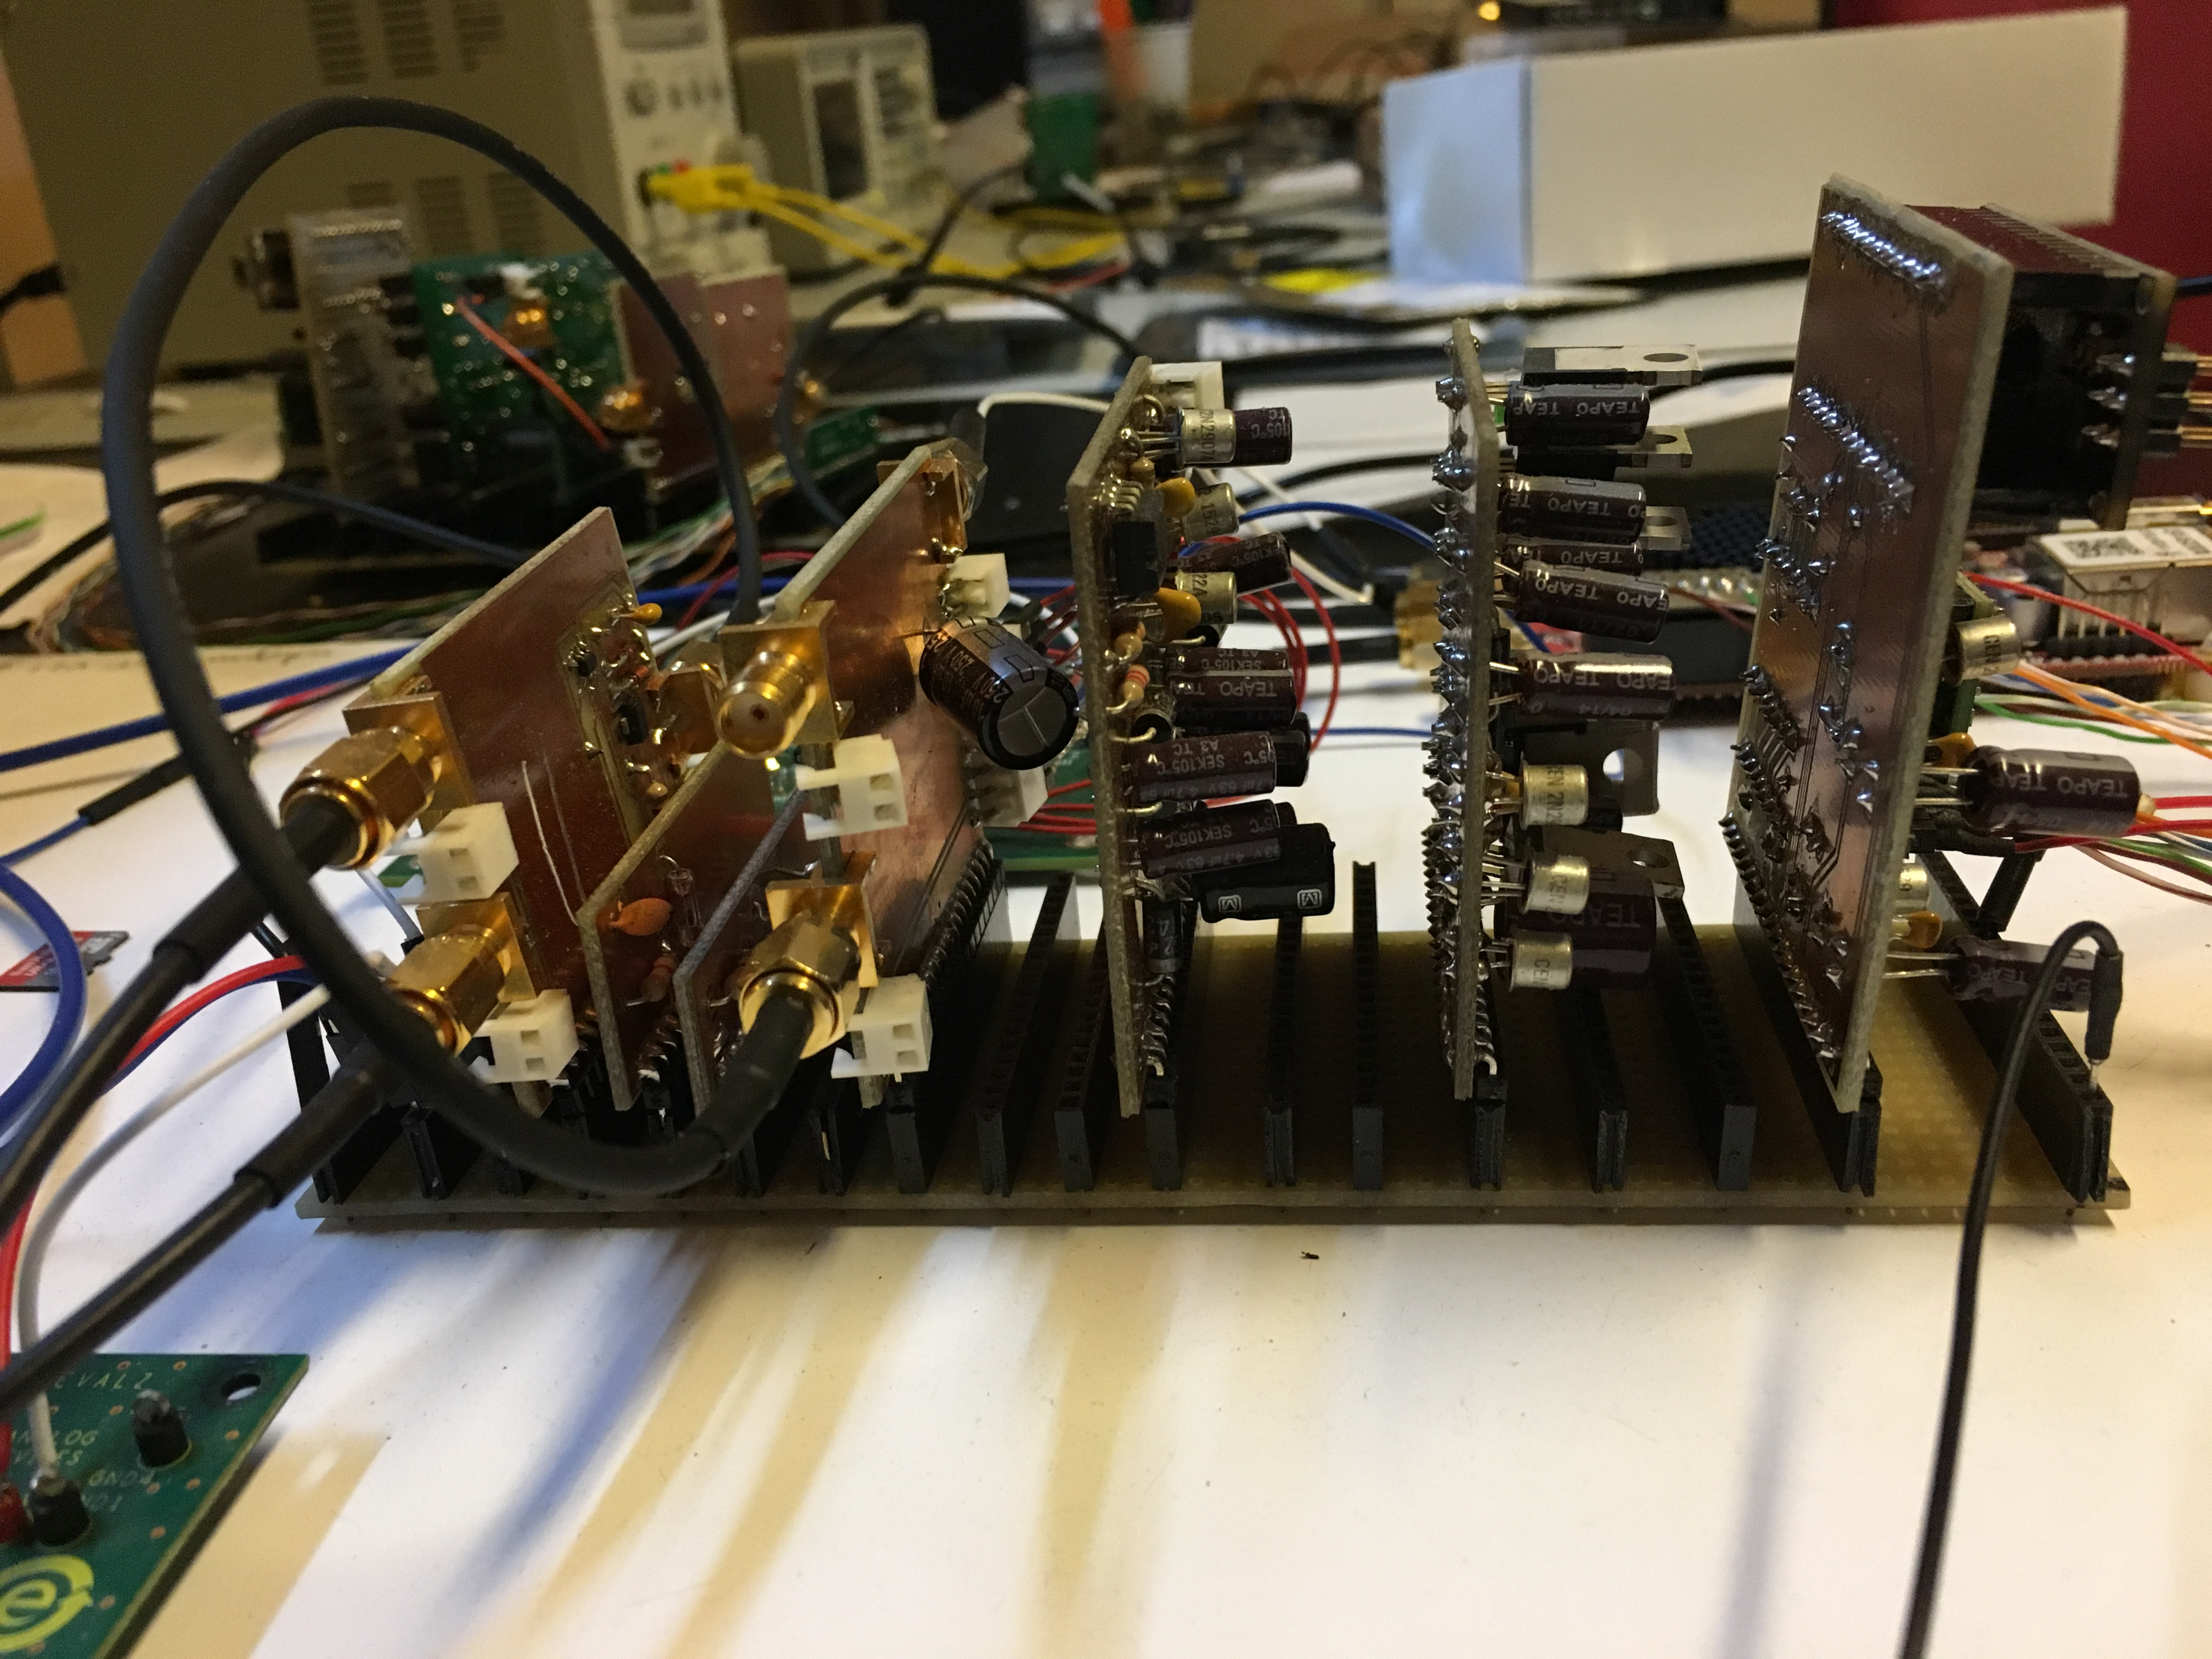
\includegraphics[width=7cm,height=5cm,trim=3cm 19.8cm 10cm 3.3cm, clip=true]{Images_Rapport/stacks}
  \end{center}
  \vspace{-5pt}
  \caption{Première version d'un kit modulable}
  \vspace{-10pt}
\end{wrapfigure}

\vspace{30pt}
La chaine d'informations du système présentant des fonctions classiques pour la filière STI2D (amplification, filtrage) mais aussi plus spécifiques (amplification à gain variable, détection d'enveloppe) elle est adaptée à une étude lors de l'enseignement de spécialité SIN plutôt que de tronc commun. Toutefois elle sera menée en parallèle ou à la suite directe des enseignemens de tronc commun sur la structure d'une chaine d'information et les premiers contacts avec la conversion analogique numérique. \par 
\vspace{30pt}

La séquence proposée vise un public de première STI2D au cours de l'enseignement de spécialité SIN. Elle prend place au second semestre à la rentrée des vacances de février. Dans l'hypothèse d'une classe de STI2D composée de 30 élèves ayant choisit pour moitié l'ensignement de spécialité ITEC et pour moitié la spécialité SIN cette séquence concerne un public de 15 élèves. L'encadrement est par conséquent réalisé par un seul enseignant. La séquence est développée sur trois semaines. En première l'enseignement de spécialité est alloué d'un volume horaire de 5 heures hebdomadaires que je divise en deux séances de 2h et 3h. En ajoutant une heure d'accompagnement personnalisé en fin de séquence on atteint un volume horaire total de 16h. \par 
\vspace{10pt}

L'ensemble de la séquence est construite autour d'un mini-projet dont le support est la sonde echOpen. On adoptera donc une approche générale inductive. 


\vspace{20pt}
\begin{center}


\begin{tabular}{|>{\bf}l|c|} \hline
Niveau d'enseignement & Première STI2D : Spécialité SIN  \\ \hline
Effectif  & 16 élèves \\\hline 
Encadrement  & 1 enseignant technologique \\\hline 
Volume horaire  & 16 h \\\hline 
Planning  & Deux séances de 2h et 3h durant 3 semaines \\\hline 
Approche  & Inductive autour d'un mini-projet \\\hline 



\end{tabular}
\end{center}


\newpage

\subsubsection{Plan détaillé de la séquence}

L'ojectif principal de cette séquence est d'amener les élèves à bien maitriser l'ensemble de la chaine d'acquisition d'un capteur de celui-ci jusqu'a la numérisation tout en les sensibilisant au thème sociétal qu'est la santé et plus précisement sa protection. L'approche par projet vise à donner de l'autonomie aux élèves en les amenant à effectuer des choix personnels, c'est le prolongement naturel des activités pratiques réalisées en enseignement transversal. De plus le support de projet est idéal si la séquence intervient dans les semaines suivant les enseignements de sciences physiques sur les ondes sonores et ultrasonores et les quelques notions d'analyse médicale.\par
\vspace{10pt}

D'un point de vue des textes officiels la séquence est construite sur les points suivants:\par
\vspace{15pt}




\begin{tabular}{|>{\bf}l|c|p{8cm}|} \hline
Item du bulletin officiel & Référence & Précisions \vspace{5pt} \\ \hline
Thème sociétal & Santé & Permettre d'investiguer les différents paramètres de santé sans intrusion. \\\hline 
\multirow{2}{*}{Centres d'intérêt}  & CI 2   & Intrumentation/Acquisition et restitution de grandeurs physiques.\vspace{5pt} \\ & CI 6 & Traitement analogique de l'information\vspace{5pt}\\\hline 
\multirow{3}{*}{Objectifs}  & CO7.sin2 & Caractérisation de fonction \vspace{5pt}\\ & CO8.sin1 & Choix de solution matérielle \vspace{5pt}\\ & CO9.sin2 & Configuration d'un système réel. \vspace{5pt}\\\hline 
\multirow{3}{*}{Prérequis}  & P-C 1.8 & Quelques outils de diagnostic médical \vspace{5pt}\\ & P-C 1.9.5 & Ondes sonores \vspace{5pt}\\ & ETT 2.1.2 & Organisation fonctionnelle d'une chaine d'information \\\hline  




\end{tabular}

\vspace{20pt}

Du point de vue des connaissances et compétences attendues en fin de séquence on trouve:\par
\vspace{20pt}

\begin{tabular}{|p{7.2cm}|p{8cm}|} \hline
\textbf{Connaissances} & \textbf{Compétences} \vspace{5pt} \\ \hline
Architecture de la chaine d'information Niveau taxonomique 2&  \textbf{Identifier} la fonction définie par un besoin exprimé \vspace{5pt} \\ \hline
Acquisition, conditionnement et filtrage d'une information analogique \par Niveau taxonomique 2 &  \textbf{Rechercher et choisir} une solution matérielle au regard de la définition d'un système \vspace{5pt} \\ \hline

Conversion analogique numérique\par Niveau taxonomique 3 &  \textbf{Connaitre} les principes et enjeux de la numérisation \vspace{5pt} \\ \hline

Adaptation d'une chaine d'acquisition aux caractéristiques des grandeurs à acquérir\par Niveau taxonomique 3 &  \textbf{Mettre en oeuvre} la chaine d'acquisition.  \vspace{5pt} \\ \hline




\end{tabular}

\newpage 

La séquence s'intitule \textbf{\underline{"Bien acquérir l'information : un problème vital !}"} et le détail des séances qui la composent est le suivant:\par
\vspace{15pt}
\color{red}
\textbf{\underline{Séance 1 : Séance d'activation - Lundi matin 8h/10h}}\par
\vspace{10pt}

\begin{adjustwidth}{5em}{0pt}
\color{blue}
\hspace{20pt}\textbf{\underline{Introduction professeur (30min):}}\par
\vspace{10pt}
\color{black}
Le professeur présente le thème de la séquence tout en l'introduisant comme la continuité logique des enseignements de la semaine précédente en enseignement transversal. Il présente ensuite rapidement le déroulement des semaines à venir puis enchaine sur le travail demandé lors de la séance du jour.\par
\vspace{10pt}


\color{blue}
\textbf{\underline{Recherches documentaires (1 heure):}}\par
\vspace{10pt}
\color{black}
Les élèves en binômes (1 trinôme) utilisent les postes réseaux afin de rechercher sur internet des éléments d'actualité et médiatiques mêlant santé et électronique (ex: coeur artificiel, imagerie médicale, pacemaker, ...). L'objectif est de les sensibiliser à la multiplicité des applications électroniques dans le domaine médical et aux progrès de la médecine grâce à elles. L'utilisation du web permet la visualisation de vidéos et autres représentations graphiques motivantes pour les élèves et induisant normalement une volonté d'en connaitre plus dans le domaine durant la séquence.\par
\vspace{10pt}

\color{blue}
\textbf{\underline{Synthèse de l'activité de recherche (30 minutes):}}\par
\vspace{10pt}
\color{black}
Les élèves se regroupent et indiquent au professeur les systèmes qu'ils ont trouvé. Le professeur les recense au tableau tout en listant leurs caractéristiques principales. L'objectif est de montrer aux élèves les différences et points communs des systèmes trouvés et d'y identifier certaines fonctions qu'ils connaissent déjà via d'autres supports. 

\end{adjustwidth}
\vspace{15pt}

\textbf{\underline{Séance 2 : Travaux dirigés - Jeudi matin 8h/11h}}\par
\vspace{10pt}

\begin{adjustwidth}{5em}{0pt}
\color{blue}
\hspace{20pt}\textbf{\underline{Travail dirigé sur l'Hemomixer (2 h 30min):}}\par
\vspace{10pt}
\color{black}
\end{adjustwidth}
\color{black}
\begin{wrapfigure}[14]{r}{0.5\textwidth}
  \vspace{-30pt}
  \hspace{-0pt}
  \begin{center}
    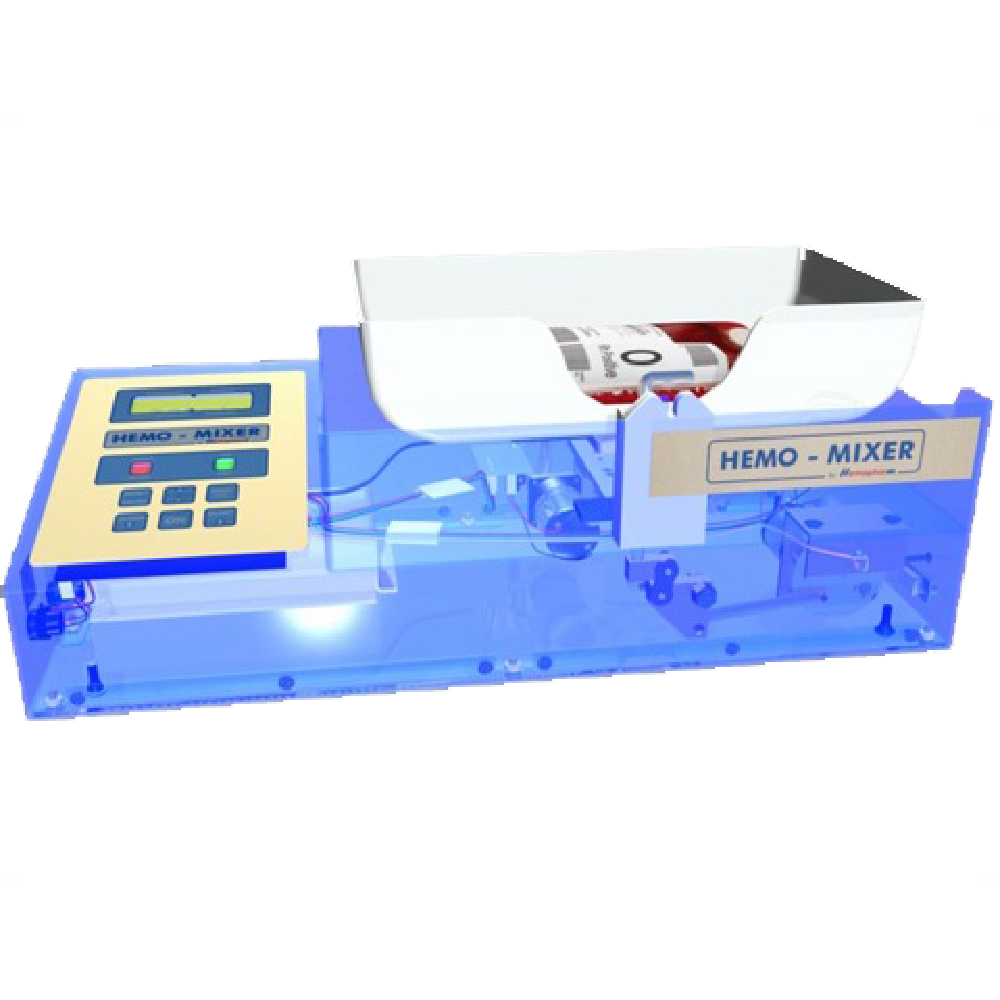
\includegraphics[width=7cm,height=5cm,trim=0cm 0cm 0cm 0cm, clip=true]{Images_Rapport/hemomixer}
  \end{center}
  \vspace{-5pt}
  \caption{Le système Hemomixer}
  \vspace{-10pt}
\end{wrapfigure}




L'Hemomixer est le système didactisé de la société didastel correspondant au thème sociétal de la santé. Il comporte la chaine de conditionnement d'un capteur de pesée ainsi que plusieurs convertisseurs analogiques numériques. L'objectif de cette séance de travaux dirigés est de renforcer les connaissances déjà acquises en tronc commun et de donner confiance aux élèves pour les projets de la semaine suivante en ayant vu récemment un cas pratique avec le groupe classe et le professeur. Les questions du TD sont orientées de manière à étudier l'organisation générale de la chaine d'information, la justification d choix d'un convertisseur analogique numérique et enfin les éléments perturbateurs des capteurs (parasitage, sensibilité, défaut de linéarité,...) 
\par




\newpage

\begin{adjustwidth}{6.5em}{0pt}
\color{blue}
\textbf{\underline{Synthèse du TD et présentation des projets (30 min):}}\par
\vspace{10pt}
\color{black}

Le professeur élabore une liste des points clés à retenir de la structure étudiée lors du TD en ayant à l'esprit le projet de la semaine suivante. Ensuite on évoque les mini-projets, le support, l'objectif à atteindre. On forme trois groupes de cinq élèves dont un est désigné chef d'équipe pour les mini-projets.

\end{adjustwidth}
\par
\vspace{30pt}

\color{red}
\textbf{\underline{Séance 3 : Mini projet partie 1 - Lundi matin 8h/10h}}\par
\vspace{10pt}
\color{black}
\textbf{Le descriptif détaillé du mini-projet est disponible à la sous-section suivante.}

\vspace{20pt}
\begin{adjustwidth}{6.5em}{0pt}
\color{blue}
\textbf{\underline{Etude de dossier technique (1 h 45 min):}}\par
\vspace{10pt}
\color{black}
La première séance du mini-projet est basée sur l'étude du dossier technique fournit par le professeur. Il s'agit de s'approprier le système, de reconnaitre les similitudes avec ce qui à été vu en TD et de proposer de premières idées en rapport avec la problématique. \par
\vspace{15pt}

\color{blue}
\hspace{-20pt}\textbf{\underline{Evaluation formative (15 min):}}\par
\vspace{10pt}
\color{black}
Le professeur passe en fin de séance dans chaque groupe et évalue par de brèves questions orales l'envie des élèves ainsi que leur compréhension du cahier des charges et leurs premières idées. Il réoriente les élèves en cas de nécessité. A ce stade il ne possède qu'une information qualitative de l'implication des groupes mais cette première impression sera combinée avec les évaluations formatives des autres séances de projet.
\end{adjustwidth}

\vspace{20pt}

\color{red}
\textbf{\underline{Séance 4 : Mini projet partie 2 - Jeudi matin 8h/11h}}\par
\vspace{10pt}
\color{black}


\vspace{20pt}
\begin{adjustwidth}{6.5em}{0pt}
\color{blue}
\textbf{\underline{Investigations (2 h 45 min):}}\par
\vspace{10pt}
\color{black}
La seconde séance de mini-projet qui constitue réellement le coeur de celui-ci. C'est durant cette séance que les élèves qui se sont réparti les tâches pratiquent leurs investigations, mesures et simulations afin de faire un choix définitif de solutions. Une bonne organisation lors de cette séance est primordiale afin de ne pas se disperser, ainsi il est important que le professeur effectue des passages réguliers dans les groupes même si il n'est pas sollicité. \par
\vspace{15pt}

\color{blue}
\hspace{-20pt}\textbf{\underline{Evaluation formative (15 min):}}\par
\vspace{10pt}
\color{black}
A la fin de cette deuxième séance de projet une nouvelle série de questions est posée à chaque groupe dans le vérifier qu'ils ont bien saisi l'ensemble des démarches effectuées ainsi et qu'ils ont bien réagit suite aux éventuelles réorientations de fin de première séance. Cette évaluation combinée avec les impressions de fin de première séance donnent désormais l'orientation de la note de projet qui sera attribuée à l'issu de l'évaluation sommative. 
\end{adjustwidth}

\vspace{20pt}

\color{red}
\textbf{\underline{Séance 5 : Mini projet partie 3 - Lundi matin 8h/10h}}\par
\vspace{10pt}
\color{black}


\vspace{20pt}
\begin{adjustwidth}{6.5em}{0pt}
\color{blue}
\textbf{\underline{Finalisation et validation du projet (2h):}}\par
\vspace{10pt}
\color{black}
La troisième et dernière séance du mini-projet sert éventuellement à terminer rapidement les dernières mesures mais il faut ensuite rapidement passer à la validation de la structure réalisée afin de pouvoir ensuite regrouper les résultats et démarrer la préparation d'un support numérique de présentation des solutions envisagées et finalement retenues. \par
 
\end{adjustwidth}







\vspace{20pt}

\color{red}
\textbf{\underline{Séance 6 : Evaluation et synthèse - Jeudi matin 8h/11h}}\par
\vspace{10pt}
\color{black}


\vspace{20pt}
\begin{adjustwidth}{6.5em}{0pt}
\color{blue}
\textbf{\underline{Evaluation sommative (1 h 30 min):}}\par
\vspace{10pt}
\color{black}
 
L'évaluation sommative pour cette séance est constituée d'une présentation orale de chaque groupe d'une durée de 15 minutes suivie de 15 minutes de questions visant à vérifier la bonne compréhension du travail effectué par l'ensemble des membres du projet. 
 \par

\vspace{20pt}
\color{blue}
\hspace{-20pt}\textbf{\underline{Synthèse de fin de séquence (1 h 30 min):}}\par
\vspace{10pt}
\color{black}
Le professeur reprend la main et après un débriefing des présentations de projet évoque les points clés à retenir de la séquence. Il distribue la fiche de synthèse regroupant l'ensemble des relations pertinentes vues au cours de la séquence. Il peut en plus distribuer une seconde fiche regroupant les points abordés mais qui entrent dans la catégorie "pour aller plus loin" afin que les élèves marquent bien la différence entre l'essentiel et les apports supplémentaires de culture générale.



 
\end{adjustwidth}


\vspace{20pt}
\renewcommand{\arraystretch}{1.8} 
\setlength{\tabcolsep}{1mm} 


\begin{figure}[!h]
\hspace{-40pt}
\begin{tabular}% 
{|>{\bfseries}l|p{1.8cm}|p{1.5cm}|p{1.5cm}|p{1.5cm}||p{1.5cm}|p{1.5cm}|p{1.5cm}|p{1.5cm}|p{1.5cm}|p{1.5cm}|p{1.5cm}|} \cline{2-11}
\multicolumn{1}{c|}{} & \scriptsize Orthographe \par \centering/2 &
\scriptsize Lisibilité \par \centering /2 &\scriptsize Clarté des explications  /2 & \scriptsize Réponses aux questions \par \centering /2 &\scriptsize Implication \par \centering /4 &\scriptsize Nature des signaux \par \centering /2 & \scriptsize Cohérence structure \par \centering /2 &\scriptsize Fonctions de base  \par \centering /2 & \scriptsize CAN \par \centering /2 & \scriptsize Total /20\\ \hline
Elève 1 & &&&&&&&&&   \\\hline Elève 2 &  & &&&&&&&&  \\\hline Elève 3 & & &&&&&&&& \\\hline Elève 4 & & &&&&&&&& \\\hline Elève 5 & & &&&&&&&& \\\hline \end{tabular}
\caption{Proposition de grille d'évaluation pour les présentations orales}
\end{figure}

\newpage

\subsubsection{Descriptif du mini-projet}

Le guide d'accompagnement de STI2D présente sous la forme d'un tableau les objectifs et modalités de réalisation d'un mini-projet technologique.\par
\vspace{10pt}

\begin{figure}[!h]
\centering
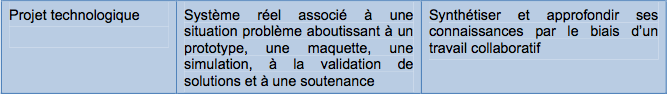
\includegraphics[width=14cm,height=2.5cm,trim=0cm 0cm 0cm 0cm, clip=true]{Images_Rapport/projet}
\caption{Un projet en filière STI2D}
\end{figure}

L'orientation que je souhait donner à ce projet entre exactement dans ce cadre. Le support utilisé est le suivant.

\begin{figure}[!h]
\centering
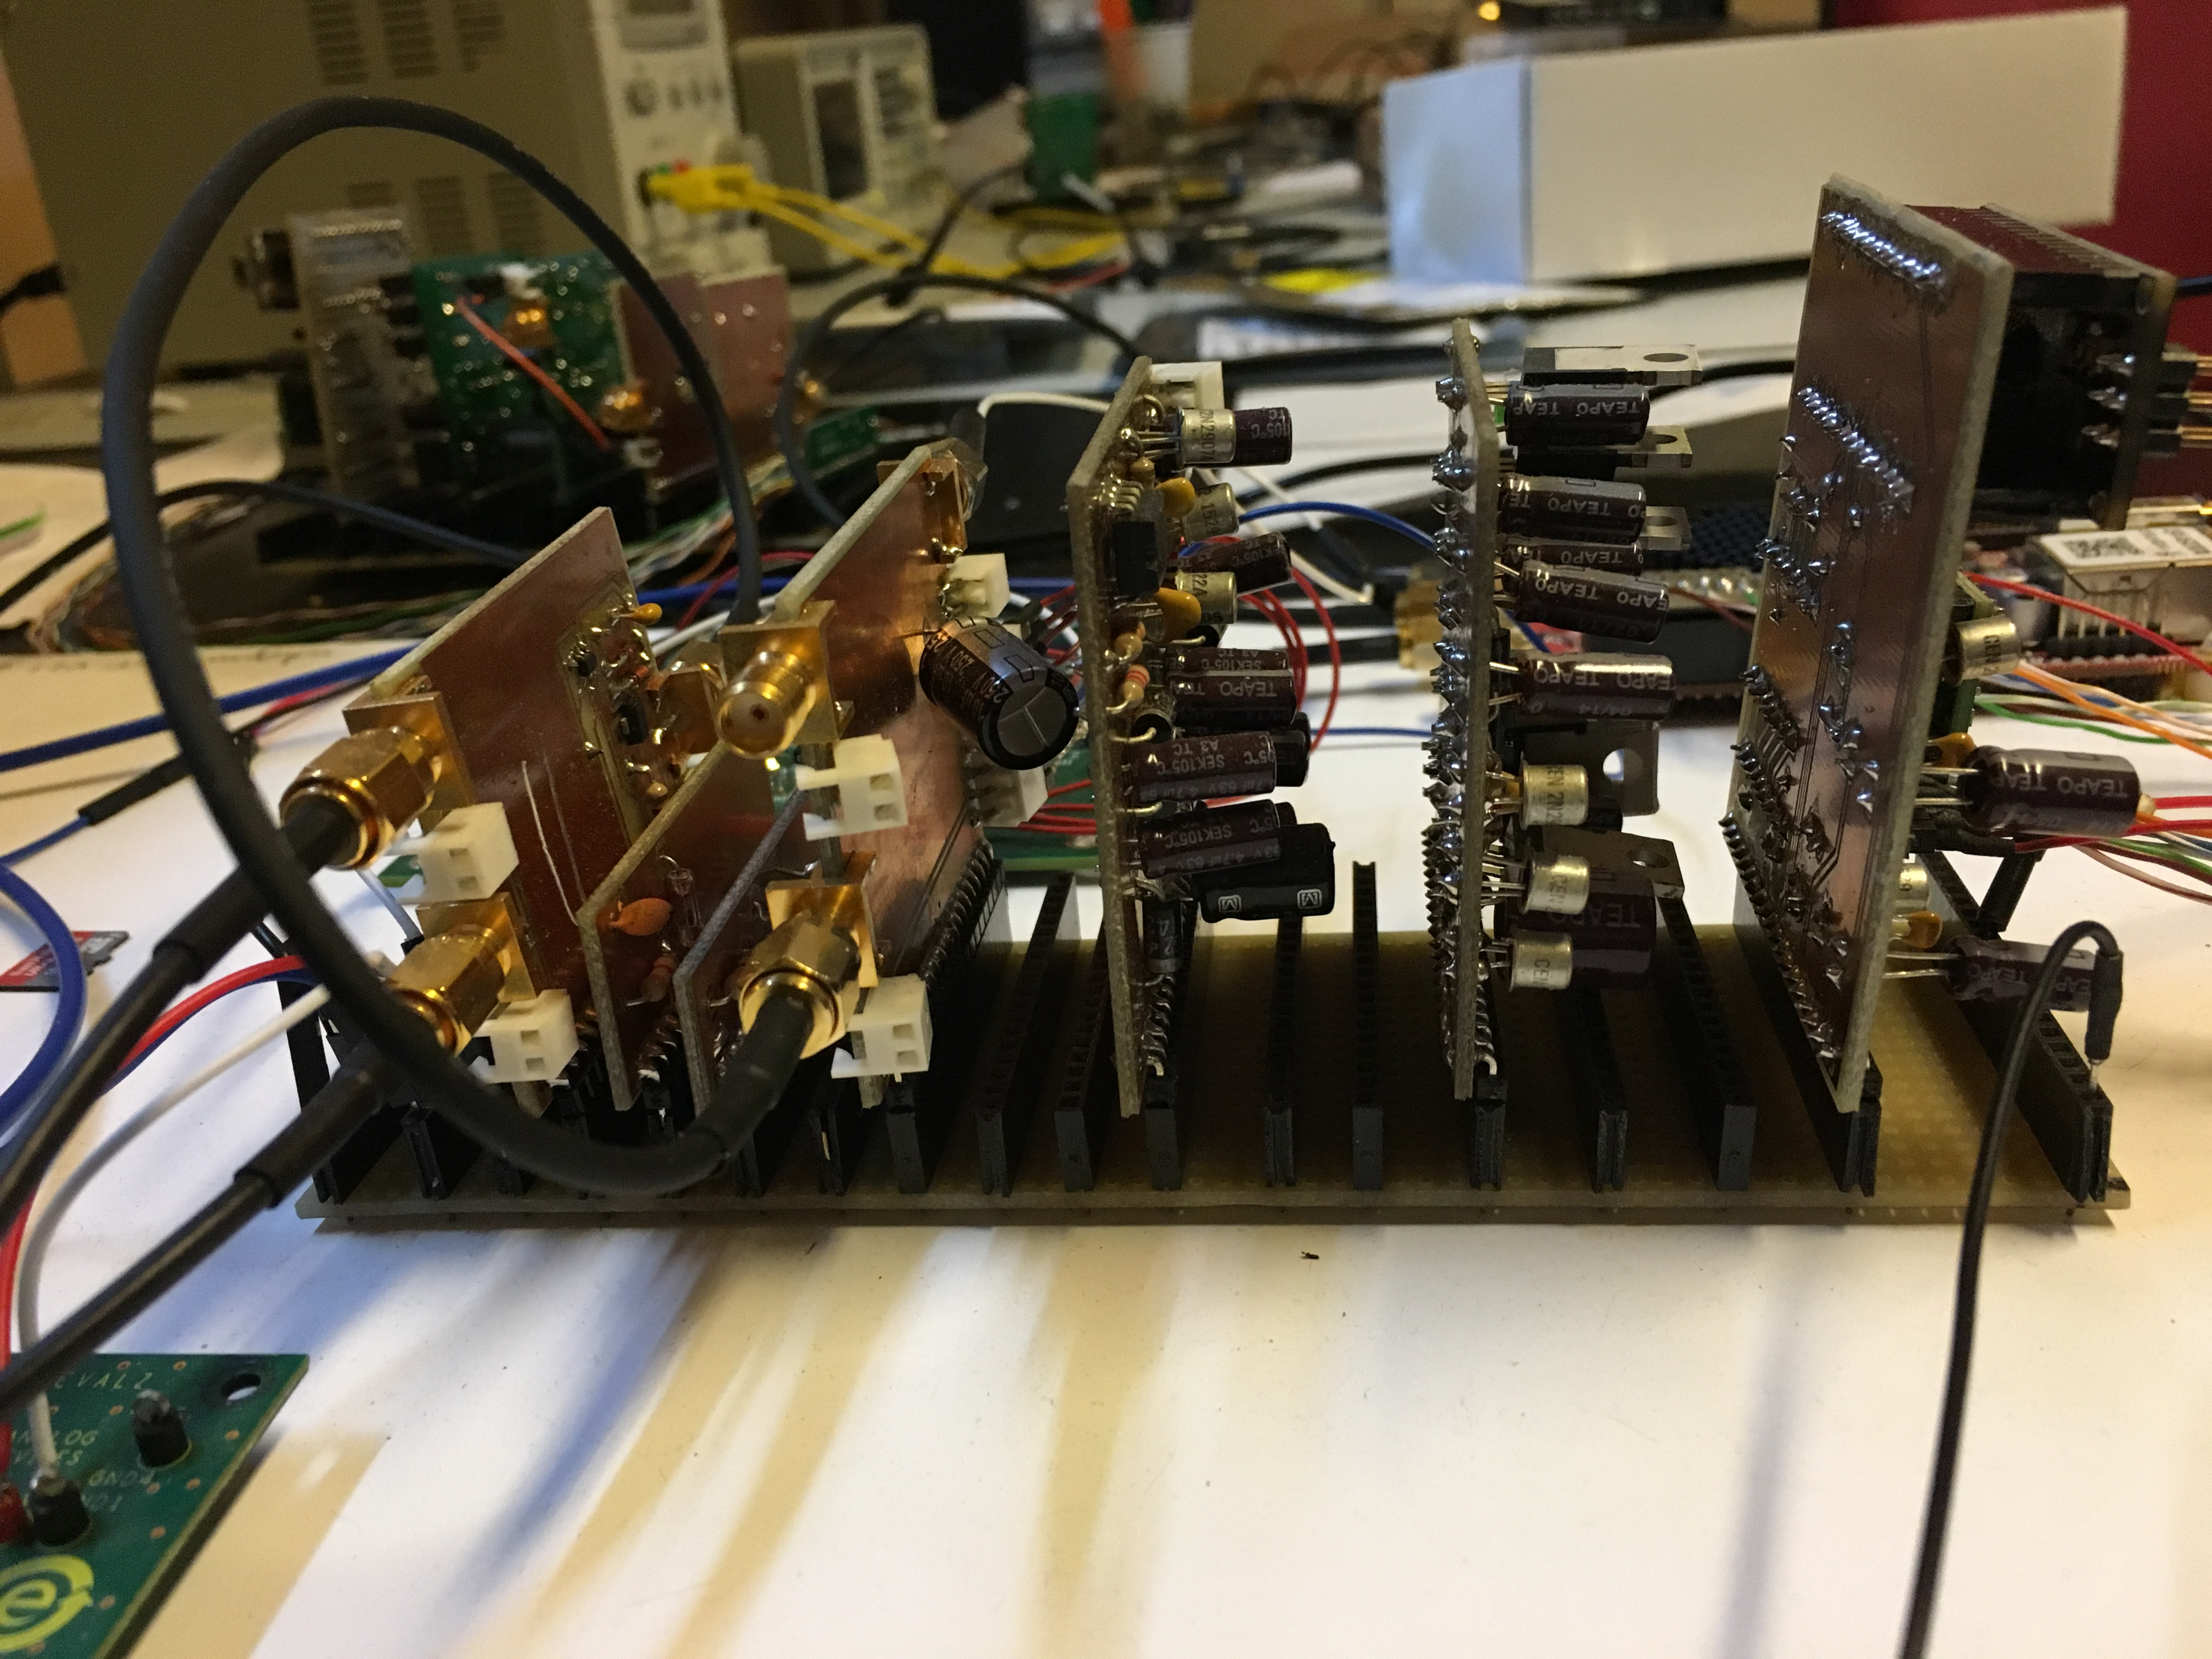
\includegraphics[width=14cm,height=8cm,trim=0cm 0cm 0cm 0cm, clip=true]{Images_Rapport/stacks}
\caption{Le système support : écho-stéthoscope sous forme de modules}
\end{figure} 

Le système est fait de telle manière à ce qu'une interaction totale soit possible. Ainsi il est possible de retirer un module et d'en enficher un autre réalisant la même fonction à sa place. C'est la fonctionnalité qui est utilisée lors de ce projet. \par
\vspace{10pt}

\textbf{L'objectif} pour les élèves est de partir du système auquel on a retiré l'ensemble des modules assurant les fonctions entre le capteur et le convertisseur analogique numérique. Ils doivent alors collaborer entre eux par groupe de cinq afin de proposer une solution matérielle fonctionnelle en fin de projet. Pour cela on met à leur disposition plusieurs modules pour chaque fonction à réaliser ainsi on conserve une démarche entière de conception tout en s'affranchissant de l'étape de réalisation de PCB qui est chronophage.

\newpage


La démarche effectuée tout au long de ce projet est donc \textbf{une démarche de créativité}.
\begin{figure}[!h]
\centering
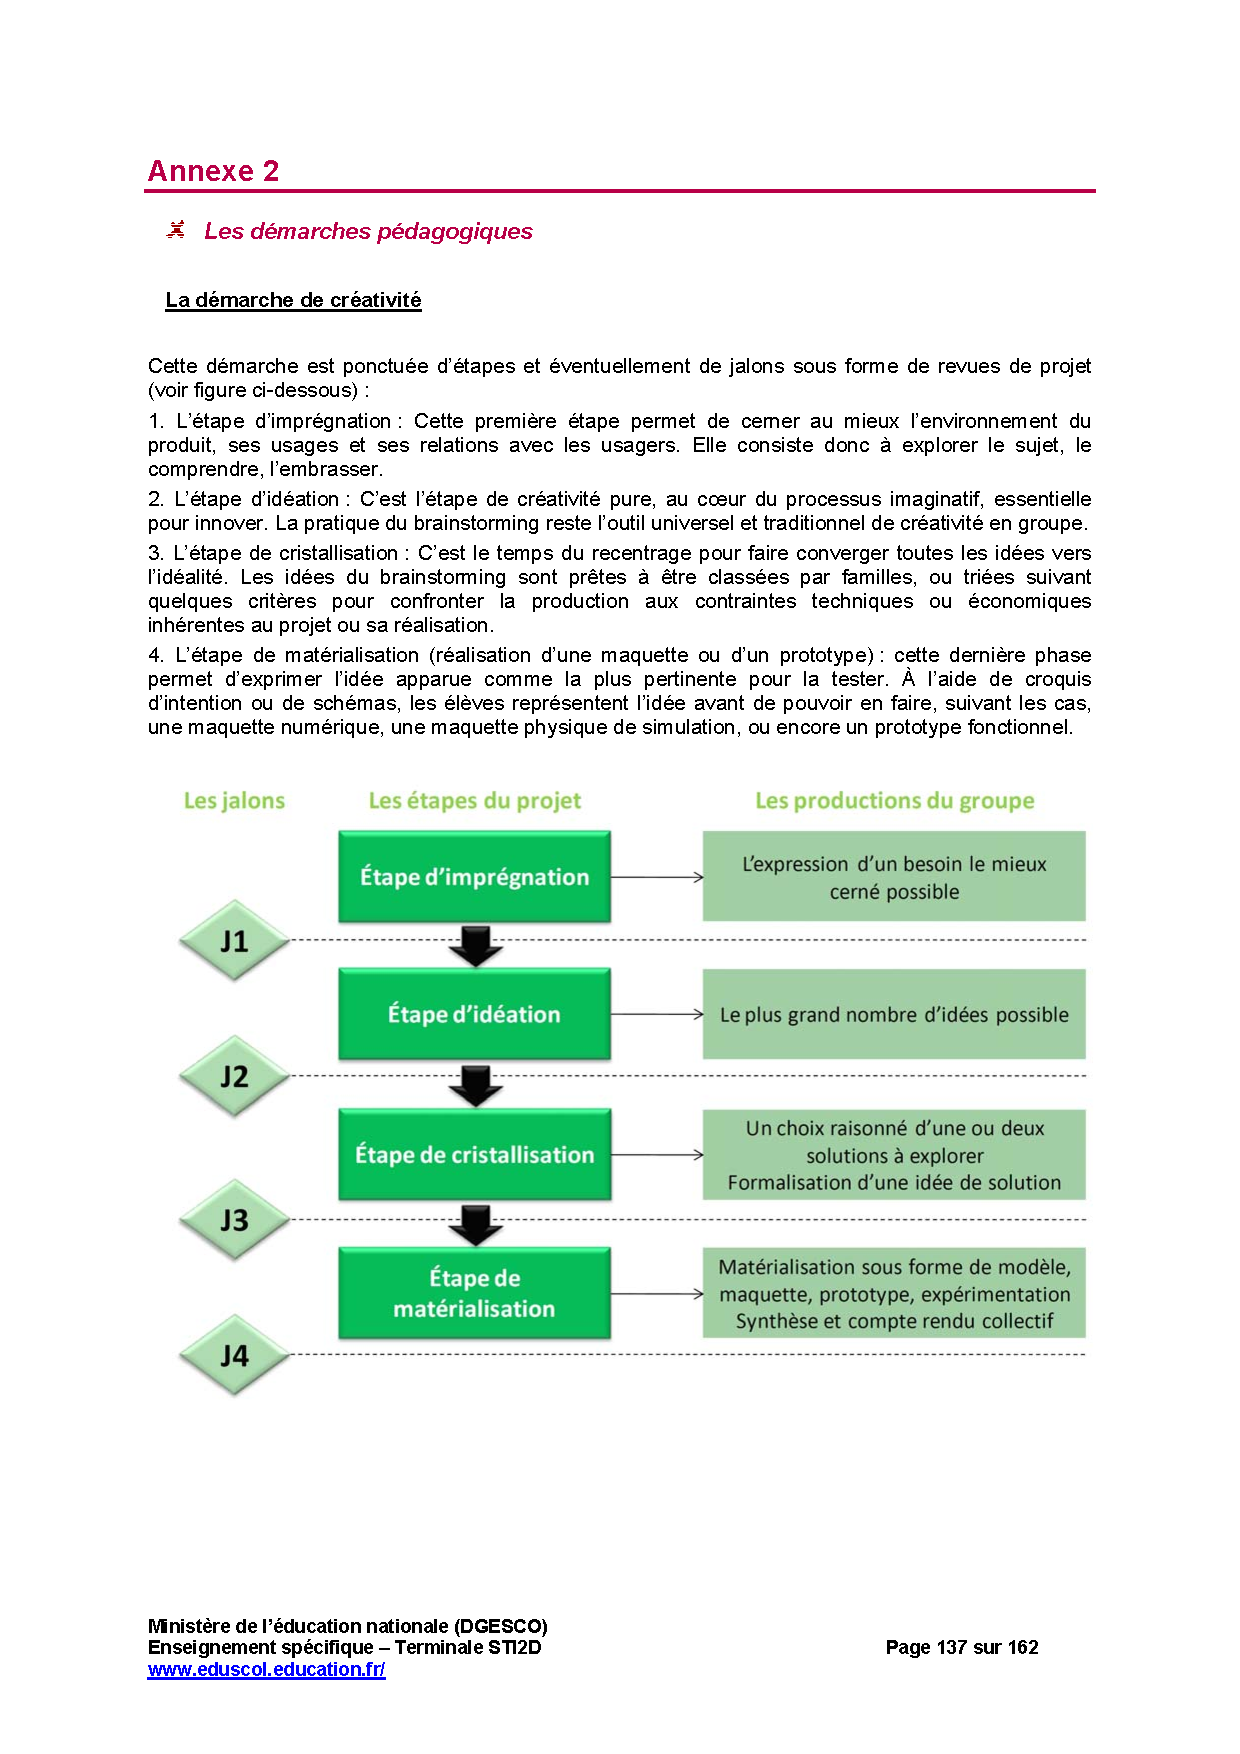
\includegraphics[width=17cm,height=9cm,trim=1cm 5cm 1cm 12.8cm, clip=true]{Images_Rapport/demarche_creativite}
\caption{Les étapes de la démarche de créativité}
\end{figure}

\vspace{10pt}

\textbf{\underline{L'étape d'imprégnation: }} Cette étape qui consiste à explorer le sujet et à le comprendre est matérialisée ici par les actions suivantes:


\begin{itemize}
\item Distribution d'un cahier technique partiel du système. Ce cahier est complet pour l'ensemble du système hormis la partie d'acquisition et de conditionnement du signal qui n'est que partiellement décrite. Il présente l'environnement du produit, ses usages et ses relations avec les usagers ce qui clarifie par exemple le fait qu'un amplificateur à gain variable soit déjà dans la chaine pour compenser l'atténuation dans les tissus biologiques.

\item  Mise à disposition de la maquette pourvue d'une chaine d'acquisition partielle.
\item Les élèves doivent relever les signaux provenant directement du capteur et étudier la documentation technique du convertisseur analogique numérique (1 modèle différent par groupe). 

\item En s'inspirant de la structure étudiée en travaux dirigés, en demandant éventuellement des précisions à l'encadrant et en utilisant les mesures faites et le cahier technique les élèves doivent normalement avoir cerné du mieux possible le besoin et franchissent alors le premier jalon.

\end{itemize}

\vspace{10pt}

\textbf{\underline{L'étape d'idéation : }} C'est l'étape ou la créativité des élèves s'exprime. En s'aidant de leurs connaissances personnelles ainsi que des moteurs de recherche à leur disposition ils se concertent afin de proposer le maximum d'idées possible. C'est également l'étape ou l'organisation en ilots commence à prendre son sens. On multiplie les points de vue et les idées lors d'un brainstorming. L'élève désigné chef de groupe à alors la responsabilité de rassembler les idées sur un tableau blanc placé devant chaque ilot de façon à mieux faire se remémorer chaque idée et ensuite les partager avec l'enseignant.
\newpage
\begin{figure}[!h]
\centering
\includegraphics[width=14cm,height=10cm,trim=0cm 0cm 0cm 0cm, clip=true]{Images_Rapport/ilot}
\caption{Un exemple de disposition d'ilôt}
\end{figure}

\vspace{20pt}

La fin de cette deuxième étape est marquée par le jalon 2 qui correspond dans notre cas à la première évaluation formative. Nous sommes alors à la fin de la première séance de projet et le professeur présente les modules dont les caractéristiques sont les plus proches de celles proposées par les étudiants.\par
\vspace{20pt}

\textbf{\underline{L'étape de cristallisation : }} Dès le début de la deuxième séance les élèves font le choix d'au maximum deux modules par fonction qu'ils veulent réaliser. Ils utilisent désormais l'ensemble des moyens mis à leur disposition (mesures, simulations par gabarit pour les filtres,...) afin de caractériser au mieux ces modules  et de vérifier qu'ils conviennent bien. Une fois les modules validés les élèves réfléchissent à l'ordre précis dans lequel ils veulent les aligner. \par
Si un groupe est particulièrement performant et semble en avance étant donné que nous sommes en spécialité il est possible de leur demander de comprendre le principe des fonctions moins communes comme l'amplificateur à gain variable (observation de sa loi de commande) ou encore le détecteur d'enveloppe analogique (ceci constituerait une première mise en contact avec un circuit qu'il retrouveront lors des l'étude de la démodulation d'amplitude plus tard dans leur cursus).\par
A la fin de cette séance on atteint le troisème jalon. La seconde évaluation formative vient alors valider le bon avancement du projet et le professeur offre normalement son aval au montage de la maquette et aux tests de fonctionnement en début de troisième séance.\par
\vspace{20pt}


\textbf{\underline{L'étape de matérialisation : }} L'étape la plus valorisante du point de vue de l'élève, c'est à ce moment qu'il voit le fruit de son travail. La validation du projet est faite par des mesures des signaux d'entrée et de sortie de chacun des modules insérés dans la chaine complète ainsi que d'un test de fonctionnement de la sonde complète sur un volontaire. \par
\vspace{10pt}

Pour vérifier le bon fonctionnement global et apporter ainsi un aspect encore plus attrayant aux élèves j'ai été amené à développer au cours de ma présence chez echOpen un programme Matlab qui remplace totalement le téléphone portable puisqu'il se connecte via wi-fi à la sonde et récupère les informations numérisées. A partir de là, le programme effectue des opérations de traitement du signal et affiche sur l'écran du PC en temps réel le signal brut récupéré, l'enveloppe du signal pour que les élèves fassent le lien avec leurs leçons de sciences physiques dans lesquels ils ont appris l'importance de l'énergie du signal et enfin l'image reconstituée de l'organe sondé. 

\begin{figure}[!h]
\centering
\includegraphics[width=15cm,height=7cm,trim=1.5cm 7cm 2cm 6cm, clip=true]{Images_Rapport/releve}
\caption{Signaux visualisés : en bas le signal récupéré, en haut son enveloppe}
\end{figure}

\begin{figure}[!h]
\centering
\includegraphics[width=9cm,height=7cm,trim=6cm 8cm 3cm 7cm, clip=true]{Images_Rapport/main}
\caption{Image obtenue : ici une vue en coupe d'une main}
\end{figure}


La séance s'achève par le début de la réalisation du support de présentation des élèves. Sont attendus dans cette présentation une description des choix effectués, un diagramme montrant la structure finale de la chaine réalisée et précisant les choix technologiques, les mesures les plus caractéristiques et enfin une image d'une main par exemple. Cette présentation qui sera évaluée durant la séance suivante représente le quatrième et dernier jalon de la démarche de créativité.

\newpage

\subsubsection{Résumé de la séquence}

La figure suivante résume l'ensemble de cette séquence à l'aide de l'outil logiciel pySequence.

\begin{figure}[!h]
\centering
\includegraphics[width=18cm,height=21cm,trim=0cm 0cm 0cm 0cm, clip=true]{Images_Rapport/pysequence}
\caption{Résumé de la séquence pédagogique en STI2D SIN}
\end{figure}


\newpage  
\subsection{Exploitation pédagogique en DUT GE2I}

\subsubsection{Structure générale de la séquence}

Cette seconde séquence pédagogique vise à intégrer la seconde partie de mon travail scientifique à savoir le dimensionnement d'une alimentation à découpage.\par

\vspace{10pt}

Il s'agit du module \textbf{Conversions d'énergie (2)} (Référence M 3101 (Ener 3)) appartenant à l'unité d'enseignement 31 "Composants, systèmes et applications" et placé au troisième semestre de la formation des étudiants en \textbf{I.U.T GEII} (Génie électrique et informatique industrielle). \par

\vspace{10pt}
\fbox{\parbox{\textwidth}{\underline{Objectif du module : } Approfondir la culture technique nécessaire pour comprendre le fonctionnement et les enjeux des convertisseurs d'énergie électrique.}}\par
\vspace{10pt}

A l'issu du module les étudiants auront normalement acquis les compétences suivantes:\par
\vspace{10pt}

\begin{itemize}
\item Analyser et mettre en oeuvre les systèmes électroniques de conversion et de transformation de l'énergie.
\item Réaliser le bilan de puissance d'un équipement.
\item Exploiter les informations d'une plaque signalétique. 
\item Dimensionner un convertisseur électromécanique.
\end{itemize}

\vspace{10pt}

Ayant déjà suivi des modules traitant de l'énergie ( M 1101, M 2101, M2302 ) et possédant déjà un bagage mathématique associé à l'électricité (Grandeurs complexes, ...) le étudiants aborderons successivement les thèmes suivants:\par
\vspace{10pt}

\begin{itemize}
\item Conversion DC/DC : hacheurs et alimentations à découpage.
\item Conversion DC/AC : onduleurs de tension et leur commande en modulation de largeur d'impulsion.
\item Machines à courant alternatif : Notion de champ tournant, Machine synchrone, Machine asynchrone.
\item Association machine asynchrone et onduleur de tension.
\end{itemize}

\vspace{10pt}

Afin d'aborder l'ensemble de ces thèmes et que les compétences soient solidement ancrées à l'issue du module il ne faudra pas hésiter à mettre en oeuvre l'ensemble des moyens pédagogiques mis à disposition à savoir les outils numériques (Simulation,...), les travaux pratiques et l'environnement numérique de travail pour mettre en place des exercices en ligne notés encourageant le travail personnel des étudiants et entrant parfaitement dans le cadre de "l'apprendre autrement".\par
\vspace{10pt}

Le volume horaire alloué à ce module est de 45 heures réparties en 10 heures de cours magistraux, 14 heures de travaux dirigés et 21 heures de travaux pratiques. Il compte pour un cinquième de la note de l'unité d'enseignement "Composants, systèmes et applications" et ses modalités d'évaluations seront : $\dfrac{1}{3}$ comptes rendus de TP , $\dfrac{1}{6}$ exercices maison , $\dfrac{1}{2}$ examen final.

\newpage

\subsubsection{Détail de la séquence}

La répartition horaire des enseignements dans le supérieur n'étant pas aussi arrêtée qu'en pré-bac il est tout de même préférable que le module se déroule sur des semaines consécutives. La figure suivante montre une proposition de répartition horaire débutant à la rentrée de septembre pour les étudiants de seconde année.\par
\vspace{10pt}


\begin{figure}[!h]
\hspace{-50pt}
\includegraphics[width=20cm,height=11cm,trim=0cm 0cm 0cm 0cm, clip=true]{Images_Rapport/horaires_geii}
\caption{Répartiton horaire de la séquence en IUT GEII}
\end{figure}

Pour cette promotion je fais le choix de consiédérer une promotion d'une soixantaine d'étudiants. Ainsi les cours magistraux sont effectués en amphithéâtre puis le groupe est scindé en trois fois 20 étudiants pour les TD dispensés par trois encadrants différents.\par 
\vspace{10pt}

Le détail des séances est le suivant:\par \vspace{10pt}

\color{red}
\textbf{Semaine 1}

\begin{adjustwidth}{5em}{0pt}
\color{blue}
\hspace{20pt}\textbf{\underline{Cours 1 : 2h}}\par
\vspace{10pt}
\color{black}
Le premier cours de la séquence commence par une introduction mettant en évidence le fait que les convertisseurs d'énergie électrique sont partout. On présente par exemple le fait que la production d'électricité français est assurée par les alternateurs ou encore que des petits convertisseurs se cachent partout comme dans les chargeurs de téléphone portable par exemple.\par
\vspace{10pt}
On effectue ensuite une étude de la structure générale d'un hacheur qui exprime la réponse à un besoin. On parle alors des principaux composants de puissance (transistor IGBT, MOSFET, diode,...) et des règles d'association des sources et on aboutit à la forme finale du hacheur série.\par
On peut finir la séance par une comparaison entre alimentation à découpage et alimentation linéaire par exemple.



\color{blue}
\hspace{20pt}\textbf{\underline{TD 1 : 2h}}\par
\vspace{10pt}
\color{black}
Le TD 1 reprend les notions vues lors du premier cours. L'objectif est de valider le fonctionnement d'un hacheur un quadrant de type boost. On vérifiera particulièrement que le système possède bien un caractère survolteur et on s'intéressera aux ondulations de tension et courants.

\begin{figure}[!h]
\centering
\includegraphics[width=10cm,height=3cm,trim=0cm 0cm 0cm 0cm, clip=true]{Images_Rapport/boost}
\caption{Hacheur de type BOOST}
\end{figure} 

\end{adjustwidth}


\vspace{10pt}

\color{red}
\textbf{Semaine 2}

\begin{adjustwidth}{5em}{0pt}
\color{blue}
\hspace{20pt}\textbf{\underline{Cours 2 : 2h}}\par
\vspace{10pt}
\color{black}

Le deuxième cours commence par une extension aux hacheurs possédant deux et quatre quadrants de fonctionnement. On parle des conséquences du besoin de réversibilité sur un hacheur et on introduit alors la cellule de commutation classique (Transistor - Diode anti-parallèle).\par
La seconde partie de ce cours introduit les principaux types d'alimentations à découpage (Flyback, Forward) : leur utilisation, leurs avantages par rapport aux hacheurs simples (isolation galvanique).

\color{blue}
\textbf{\underline{TD 2 : 2h}}\par
\vspace{10pt}
\color{black}

Le deuxième TD concerne la fabrication d'un hacheur. On fournit aux élèves un cahier des charges et ils doivent en déduire la structure du hacheur qui convient (quadrants de fonctionnements, nature des interrupteurs, éventuel ajout d'inductance pour associer les sources,...) et qui soit le plus économique possible.

\end{adjustwidth}

\vspace{10pt}



\vspace{10pt}

\color{red}
\textbf{Semaine 4}

\begin{adjustwidth}{5em}{0pt}
\color{blue}
\hspace{20pt}\textbf{\underline{TD 3 : 2h}}\par
\vspace{10pt}
\color{black}
Le troisième TD se déroule en salle informatique. On fournit aux étudiants en binôme le modèle Simscape présenté en partie scientifique d'une alimentation Flyback. Les principales équations de fonctionnement étant fournies les étudiants doivent retrouver les formes d'ondes caractéristique de la structure. On leur demande ensuite à partir d'un cahier des charges de modifier judicieusement les paramètres de leur choix afin de réaliser une structure permettant d'atteindre des niveaux différents (exemple: passer d'une structure 325 $\rightarrow$ 18V à une structure 5 $\rightarrow$ 12 V).\par 
\vspace{10pt}
\newpage
\begin{figure}[!h]
\centering
\includegraphics[width=12cm,height=7cm,trim=0cm 5cm 0cm 5cm, clip=true]{Images_Rapport/flyback_simscape}
\caption{Modèle proposé aux étudiants pour les simulations}
\end{figure} 



 

\end{adjustwidth}



\vspace{10pt}

\color{red}
\textbf{Semaine 5}

\begin{adjustwidth}{5em}{0pt}
\color{blue}
\hspace{20pt}\textbf{\underline{Cours 3 : 2h}}\par
\vspace{10pt}
\color{black}

Ce cours marque le début de l'étude des convertisseurs DC/AC. Il montre aux élèves que la structure physique de l'onduleur est identique à celle d'un hacheur 4 quadrants puisque les grandeurs sont alternativement positives et négatives.\par 
Le point essentiel de ce cours est donc d'introduire la loi de commande d'un onduleur et donc le principe général de la MLI.


\color{blue}
\hspace{20pt}\textbf{\underline{TD 4 : 2h}}\par
\vspace{10pt}
\color{black}

Le sujet du quatrième TD est un onduleur monophasé en demi-pont capacitif débitant sur une charge RL. Ce TD montre que dans un montage du type la loi de commande est primordiale avec notamment le fait que le seul moyen d'équilibrer les tensions sur chaque condensateur est d'avoir un rapport cyclique moyen $\alpha = \dfrac{1}{2}$.

\begin{figure}[!h]
\centering
\includegraphics[width=8cm,height=3cm,trim=0cm 0cm 0cm 0cm, clip=true]{Images_Rapport/mipont}
\caption{Onduleur monophasé à demi pont capacitif}
\end{figure}


\end{adjustwidth}




\vspace{10pt}

\color{red}
\textbf{Semaine 6}

\begin{adjustwidth}{5em}{0pt}
\color{blue}
\hspace{20pt}\textbf{\underline{Cours 4 : 2h}}\par
\vspace{10pt}
\color{black}
Les quatrième cours est un cours préparatoire à l'étude des machines à courant alternatif. Il aborde les notions de champ tournant et de champ pulsant. On étudie la façon dont on alimente (courants triphasés équilibrés) et on place géométriquement des bobinages (répartition sinusoïdale) de façon à obtenir un champ tournant. On finit par évoquer la structure physique des machines électriques suivantes : machine asynchrone , machine synchrone à aimants permanents, machine synchrone à rotor bobiné. Les machines synchrones sont uniquement à pôles lisses.



\color{blue}
\hspace{20pt}\textbf{\underline{TD 5 : 2h}}\par
\vspace{10pt}
\color{black}
Le TD cinq est un TD de simulation avec pour objectif de mieux se représenter les principes physiques du champ tournant.

 

\end{adjustwidth}

\vspace{10pt}

\color{red}
\textbf{Semaine 7}

\begin{adjustwidth}{5em}{0pt}
\color{blue}
\hspace{20pt}\textbf{\underline{Cours 5 : 2h}}\par
\vspace{10pt}
\color{black}

Le dernier cours de la séquence concerne l'étude détaillée des machines synchrones et asynchrones. On parlera notamment de leurs applications les plus courantes, de leurs ponts communs mais aussi de leur différences. On donne les schémas équivalents monophasés des deux machines. 


\color{blue}
\hspace{20pt}\textbf{\underline{TD 6 : 2h}}\par
\vspace{10pt}
\color{black}

Le sixième TD est utilisé pour réaliser un bilan de puissance complet sur une machine asynchrone. On démarrera notamment l'étude à l'aide de la lecture de sa plaque signalétique.

\begin{figure}[!h]
\centering
\includegraphics[width=12cm,height=4cm,trim=0cm 0cm 0cm 0cm, clip=true]{Images_Rapport/plaque}
\caption{Plaque signalétique d'une machine asynchrone}
\end{figure} 



\end{adjustwidth}

\vspace{10pt}

\color{red}
\textbf{Semaine 8}

\begin{adjustwidth}{5em}{0pt}



\color{blue}
\hspace{20pt}\textbf{\underline{TD 7 : 2h}}\par
\vspace{10pt}
\color{black}

Le dernier TD exploite le schéma équivalent monophasé afin de tracer les caractéristiques de couple de la machine asynchrone et de mieux saisir les notions de glissement, de vitesse de synchronisme et d'identifier les zones de la caractéristiques dans lesquelles on travaille en pratique.



\end{adjustwidth}

\vspace{10pt}




\newpage
\color{red}
\textbf{\underline{Séances de travaux pratiques}}\par
\color{black}
\vspace{10pt}
Pour les séances de travaux pratiques l'effectif est divisé en 5 groupes de 6 binômes. Par soucis de métériel ces séances sont situées à la fin de la séquence même si elles illustrent l'ensemble de celle-ci. On propose 6 sujets de travaux pratiques sur lesquels les élèves tournent au cours des six séances de travaux pratiques de 3h30 : \par
\vspace{10pt}
\begin{itemize}
\item Commande en couple d'une machine à courant continu. Commande d'un hacheur 4 quadrants.
\item Maquettes didactisées des deux alimentations à découpage flyback/forward. Visualisation des formes d'ondes caractéristiques, vérification du fonctionnement et bilan de puissance.
\item Onduleur de tension sur charge RLC. Etude des filtres d'entrée et de sortie.
\item Identification des paramètres d'une machine synchrone.
\item Couplage d'un alternateur synchrone au réseau.
\item Variation de vitesse de la machine asynchrone.
\end{itemize}


\color{black}
\subsection{Conclusion de la partie pédagogique}

Le système de sonde échographique est un dispositif qui embarque une composante informationnelle très importante. Faisant partie du thème sociétal de la santé cela m'a permis d'en tirer une séquence pour le cycle terminal technologique centrée sur un mini-projet qui devrait intéresser les élèves car il laisse une large part à leur créativité et s'inscrit pleinement dans la spécialité SIN qu'ils ont choisit car elle correspond à leur gout.\par
En exploitant la suite de mon travail scientifique portant sur une partie singulière de la sonde qui est son système d'alimentation j'ai également pu envisager une séquence pédagogique cette fois-ci orientée énergie pour le supérieur. Ces deux séquences très différentes montrent l'étendue des possibilités pédagogiques qu'offre un système du monde réel de l'industrie.\par
Il serait encore possible d'envisager d'autres pistes pédagogiques exploitant ce système en s'intéressant par exemple aux communications entre le corps de sonde et le téléphone portable ou encore au traitement numérique de l'information.


\newpage
\bibliographystyle{plain}
\bibliography{Rapport}
\newpage
\section{Annexe 1}

\begin{figure}[!h]
  \hspace{-50pt}
  \rotatebox{-90}{ \includegraphics[width=22.3cm,height = 20cm,trim=.5cm 16cm .5cm 0.5cm, clip=true]{Images_Rapport/sequence}}
 
  
  
  \caption{Diagramme de séquence}
  
\end{figure}

\end{document}










































